%%%%%%%%%%%%%%%%%%%%%%%%%%%%% Thesis.tex %%%%%%%%%%%%%%%%%%%%%%%%%%%%%%%
%                                                                      %
%  ---------- Master of Science Dissertation template ----------       %
%                                                                      %
%  Template for the Master Thesis according to the regulations         %
%  published by the Academic Board (Direcção Académica) at IST.        %
%                                                                      %
%  For up-to-date guide, please refer to the official website          %
%
% https://tecnico.ulisboa.pt/pt/ensino/estudar-no-tecnico/informacoes-academicas/dissertacao-de-mestrado/
%                                                                      %
%       Andre C. Marta                                                 %
%       Area Cientifica de Mecanica Aplicada e Aeroespacial            %
%       Departamento de Engenharia Mecanica                            %
%       Instituto Superior Tecnico                                     %
%       Av. Rovisco Pais                                               %
%       1049-001 Lisboa                                                %
%       Portugal                                                       %
%       Tel: +351 21 841 9469                                          %
%                        3469 (extension)                              %
%       Email: andre.marta@tecnico.ulisboa.pt                          %
%                                                                      %
%  Created:       Jan 20, 2011                                         %
%  Last Modified: Mar  4, 2024                                         %
%                                                                      %
%%%%%%%%%%%%%%%%%%%%%%%%%%%%%%%%%%%%%%%%%%%%%%%%%%%%%%%%%%%%%%%%%%%%%%%%
%  Revision history                                                    %
%  v1 - 2011/01/24 - original template                                 %
%  v2 - 2012/10/30 - new IST image and glossary support                %
%  v3 - 2013/12/10 - update according to 2012/13 official guide        %
%  v4 - 2014/02/28 - new default for bibliography style                %
%  v5 - 2014/05/07 - update according to 2013/14 official guide        %
%  v6 - 2015/07/02 - cover page format fixed,                          %
%                    contents page numbering fixed,                    %
%                    better language support,                          %
%                    enhanced examples of tables,                      %
%                    new option for appendix page numbering format,    %
%                    custom bibliography style                         %
%  v7 - 2018/02/19 - multiple citations compressed                     %
%  v8 - 2019/05/13 - added examples (pseudo-code)                      %
%  v9 - 2020/03/03 - added French language support                     %
%                    indented first paragraphs                         %
%  v10- 2021/01/29 - place caption above table                         %
%  v11- 2022/06/29 - included Declaration of original work             %
%  v12- 2024/02/26 - new glossaries and subfig packages                %
%%%%%%%%%%%%%%%%%%%%%%%%%%%%%%%%%%%%%%%%%%%%%%%%%%%%%%%%%%%%%%%%%%%%%%%%
%                                                                      %
% To generate the PDF file, type "make" at the terminal prompt.        %
%                                                                      %
% This IST template LaTeX package was created by the author            %
% and it can be downloaded from:                                       %
%    https://fenix.tecnico.ulisboa.pt/homepage/ist31052/               %
% or https://mdo.tecnico.ulisboa.pt/templates/                         %
%                                                                      %
% The external packages can be downloaded from                         %
% the Comprehensive TeX Archive Network at http://www.ctan.org/        %
%                                                                      %
% List of LaTex symbols:                                               %
% http://www.ctan.org/tex-archive/info/symbols/comprehensive/          %
%                                                                      %
% Help with LaTex can be found at                                      %
% http://en.wikibooks.org/wiki/LaTeX                                   %
%%%%%%%%%%%%%%%%%%%%%%%%%%%%%%%%%%%%%%%%%%%%%%%%%%%%%%%%%%%%%%%%%%%%%%%%

%%%%%%%%%%%%%%%%%%%%%%%%%%%%%%%%%%%%%%%%%%%%%%%%%%%%%%%%%%%%%%%%%%%%%%%%
%     Preamble                                                         %
%%%%%%%%%%%%%%%%%%%%%%%%%%%%%%%%%%%%%%%%%%%%%%%%%%%%%%%%%%%%%%%%%%%%%%%%

% ----------------------------------------------------------------------
%  Set the document class
% ----------------------------------------------------------------------
\documentclass[10pt,a4paper,twoside]{report}

% ----------------------------------------------------------------------
% Define external packages, language, margins, fonts and new commands
% ----------------------------------------------------------------------
%%%%%%%%%%%%%%%%%%%%%%%%%%%%%%%%%%%%%%%%%%%%%%%%%%%%%%%%%%%%%%%%%%%%%%%%
%                                                                      %
%     File: Thesis_Preamble.tex                                        %
%     Tex Master: Thesis.tex                                           %
%                                                                      %
%     Author: Andre C. Marta                                           %
%     Last modified :  4 Mar 2024                                      %
%                                                                      %
%%%%%%%%%%%%%%%%%%%%%%%%%%%%%%%%%%%%%%%%%%%%%%%%%%%%%%%%%%%%%%%%%%%%%%%%

% 'natbib' package
%
% Flexible bibliography support.
% https://www.ctan.org/pkg/natbib
%
% > produce author-year style citations
%
% \citet  and \citep  for textual and parenthetical citations, respectively
% \citet* and \citep* that print the full author list, and not just the abbreviated one
% \citealt is the same as \citet but without parentheses. Similarly, \citealp is \citep without parentheses
% \citeauthor
% \citeyear
% \citeyearpar
%
%% natbib options can be provided when package is loaded \usepackage[options]{natbib}
%%
%% Following options are valid:
%%
%%   round  -  round parentheses are used (default)
%%   square -  square brackets are used   [option]
%%   curly  -  curly braces are used      {option}
%%   angle  -  angle brackets are used    <option>
%%   semicolon  -  multiple citations separated by semi-colon (default)
%%   colon  - same as semicolon, an earlier confusion
%%   comma  -  separated by comma
%%   authoryear - for author–year citations (default)
%%   numbers-  selects numerical citations
%%   super  -  numerical citations as superscripts, as in Nature
%%   sort   -  sorts multiple citations according to order in ref. list
%%   sort&compress   -  like sort, but also compresses numerical citations
%%   compress - compresses without sorting
%%
% ******************************* SELECT *******************************
%\usepackage{natbib}          % <<<<< References in alphabetical list Correia, Silva, ...
\usepackage[numbers,sort&compress]{natbib} % <<<<< References in numbered list [1],[2],...
% ******************************* SELECT *******************************


% 'notoccite' package
%
% Prevent trouble from citations in table of contents, etc.
% http://ctan.org/pkg/notoccite
%
% > If you have \cite commands in \section-like commands, or in \caption,
%   the citation will also appear in the table of contents, or list of whatever.
%   If you are also using an unsrt-like bibliography style, these citations will
%   come at the very start of the bibliography, which is confusing. This pack­age
%   suppresses the effect.
%
\usepackage{notoccite}


% ----------------------------------------------------------------------
% Define document language.
% ----------------------------------------------------------------------

% 'inputenc' package
%
% Accept different input encodings.
% https://www.ctan.org/pkg/inputenc
%
% > allows typing non-english text in LaTeX sources.
%
% ******************************* SELECT *******************************
%\usepackage[latin1]{inputenc} % <<<<< Windows
\usepackage[utf8]{inputenc}   % <<<<< Linux
% ******************************* SELECT *******************************

% 'babel' package
%
% Multilingual support for Plain TeX or LaTeX.
% https://www.ctan.org/pkg/babel
%
% > sets the variable names according to the language selected
%
% ******************************* SELECT *******************************
%\usepackage[portuguese]{babel} % <<<<< Portuguese
\usepackage[english]{babel} % <<<<< English
%\usepackage[francais]{babel} % <<<<< French (requires package texlive-lang-french)
% ******************************* SELECT *******************************

% 'nomencl' package
%
% Produce lists of symbols as in nomenclature.
% https://www.ctan.org/pkg/nomencl
%
% The nomencl package makes use of the MakeIndex program
% in order to produce the nomenclature list.
%
% Nomenclature
% 1) On running the file through LATEX, the command \makenomenclature
%    in the preamble instructs it to create/open the nomenclature file
%    <jobname>.nlo corresponding to the LATEX file <jobname>.tex and
%    writes the information from the \nomenclature commands to this file.
% 2) The next step is to invoke MakeIndex in order to produce the
%    <jobname>.nls file. This can be achieved by making use of the
%    command: makeindex <jobname>.nlo -s nomencl.ist -o <jobname>.nls
% 3) The last step is to invoke LATEX on the <jobname>.tex file once
%    more. There, the \printnomenclature in the document will input the
%    <jobname>.nls file and process it according to the given options.
%
% Nomenclature (produces *.nlo *.nls files)
\usepackage{nomencl}
\makenomenclature
%
% Group variables according to their symbol type
% (see <prefix> in Thesis_Nomenclature.tex)
%
\RequirePackage{ifthen} 
\ifthenelse{\equal{\languagename}{english}}%
    { % English
    \renewcommand{\nomgroup}[1]{%
      \ifthenelse{\equal{#1}{R}}{%
        \item[\textbf{Roman symbols}]}{%
        \ifthenelse{\equal{#1}{G}}{%
          \item[\textbf{Greek symbols}]}{%
          \ifthenelse{\equal{#1}{S}}{%
            \item[\textbf{Subscripts}]}{%
            \ifthenelse{\equal{#1}{T}}{%
              \item[\textbf{Superscripts}]}{}}}}}%
    }{%
    \ifthenelse{\equal{\languagename}{french}}%
    { % French
    \renewcommand{\nomgroup}[1]{%
      \ifthenelse{\equal{#1}{R}}{%
        \item[\textbf{Symbole romains}]}{%
        \ifthenelse{\equal{#1}{G}}{%
          \item[\textbf{Symboles grecs}]}{%
          \ifthenelse{\equal{#1}{S}}{%
            \item[\textbf{Indices}]}{% lettre inférieure
            \ifthenelse{\equal{#1}{T}}{%
              \item[\textbf{Exposants}]}{}}}}}% lettre supérieure
    }{ % Portuguese
    \renewcommand{\nomgroup}[1]{%
      \ifthenelse{\equal{#1}{R}}{%
        \item[\textbf{Simbolos romanos}]}{%
        \ifthenelse{\equal{#1}{G}}{%
          \item[\textbf{Simbolos gregos}]}{%
          \ifthenelse{\equal{#1}{S}}{%
            \item[\textbf{Subscritos}]}{%
            \ifthenelse{\equal{#1}{T}}{%
              \item[\textbf{Sobrescritos}]}{}}}}}%
    }}%


% 'glossaries' package
%
% Create glossaries and lists of acronyms
% https://www.ctan.org/pkg/glossaries
%
% The glossaries package makes use of the MakeIndex program
% in order to produce the glossary list.
%
% The following options are used:
%   - acronym      : to produce the list of acronyms
%   - nonumberlist : to remove the page number
%   - nopostdot    : to remove the dot at the end of definition of term
%   - nogroupskip  : to remove the line spacing between groups
%
% Glossary (produces *.glo *.ist files)
%
\usepackage[acronym,nonumberlist,nopostdot,nogroupskip]{glossaries}
\setglossarystyle{long}
\renewcommand{\glsnamefont}[1]{\textbf{#1}} % acronym in bold face
\makeglossaries


% List of LaTeX variable names: \abstractname, \appendixname, \bibname,
%   \chaptername, \contentsname, \listfigurename, \listtablename, ...)
% https://texfaq.org/FAQ-fixnam
%
% Changing the words babel uses (uncomment and redefine as necessary...)
%
\newcommand{\acknowledgments}{@undefined} % new LaTeX variable name
%
% > English
%
\addto\captionsenglish{\renewcommand{\acknowledgments}{Acknowledgments}}
%\addto\captionsenglish{\renewcommand{\contentsname}{Contents}}
%\addto\captionsenglish{\renewcommand{\listtablename}{List of Tables}}
%\addto\captionsenglish{\renewcommand{\listfigurename}{List of Figures}}
%\addto\captionsenglish{\renewcommand{\nomname}{Nomenclature}} % (List of Symbols)
%\addto\captionsenglish{\renewcommand{\glossaryname}{Glossary}}
\addto\captionsenglish{\renewcommand{\acronymname}{Glossary}} % Acronyms
%\addto\captionsenglish{\renewcommand{\bibname}{References}} % Bibliography
%\addto\captionsenglish{\renewcommand{\appendixname}{Appendix}}

% > French
%
\addto\captionsfrench{\renewcommand{\acknowledgments}{Remerciements}}
%\addto\captionsfrench{\renewcommand{\contentsname}{Table des matières}}
%\addto\captionsfrench{\renewcommand{\listtablename}{Liste des tableaux}}
\addto\captionsfrench{\renewcommand{\listfigurename}{Liste des figures}} % Table des figures
%\addto\captionsfrench{\renewcommand{\nomname}{Nomenclature}}
%\addto\captionsfrench{\renewcommand{\glossaryname}{Glossaire}}
%\addto\captionsfrench{\renewcommand{\acronymname}{Liste des acronymes}}
%\addto\captionsfrench{\renewcommand{\bibname}{Bibliographie}}
%\addto\captionsfrench{\renewcommand{\appendixname}{Annexe}}

% > Portuguese
%
\addto\captionsportuguese{\renewcommand{\acknowledgments}{Agradecimentos}}
%\addto\captionsportuguese{\renewcommand{\contentsname}{Conte\'{u}do}}
%\addto\captionsportuguese{\renewcommand{\listtablename}{Lista de Figuras}}
%\addto\captionsportuguese{\renewcommand{\listfigurename}{Lista de Tabelas}}
\addto\captionsportuguese{\renewcommand{\nomname}{Lista de S\'{i}mbolos}} % Nomenclatura
%\addto\captionsportuguese{\renewcommand{\glossaryname}{Gloss\'{a}rio}}
%\addto\captionsportuguese{\renewcommand{\acronymname}{Lista de Abrevia\c{c}\~{o}es}}
%\addto\captionsportuguese{\renewcommand{\bibname}{Refer\^{e}ncias}} % Bibliografia
%\addto\captionsportuguese{\renewcommand{\appendixname}{Anexo}} % Apendice


% ----------------------------------------------------------------------
% Define cover fields in both english and portuguese.
% ----------------------------------------------------------------------
%
\newcommand{\coverThesis}{@undefined} % new LaTeX variable name
\newcommand{\coverSupervisors}{@undefined} % new LaTeX variable name
\newcommand{\coverExaminationCommittee}{@undefined} % new LaTeX variable name
\newcommand{\coverChairperson}{@undefined} % new LaTeX variable name
\newcommand{\coverSupervisor}{@undefined} % new LaTeX variable name
\newcommand{\coverMemberCommittee}{@undefined} % new LaTeX variable name
% > English
\addto\captionsenglish{\renewcommand{\coverThesis}{Thesis to obtain the Master of Science Degree in}}
\addto\captionsenglish{\renewcommand{\coverSupervisors}{Supervisor(s)}}
\addto\captionsenglish{\renewcommand{\coverExaminationCommittee}{Examination Committee}}
\addto\captionsenglish{\renewcommand{\coverChairperson}{Chairperson}}
\addto\captionsenglish{\renewcommand{\coverSupervisor}{Supervisor}}
\addto\captionsenglish{\renewcommand{\coverMemberCommittee}{Member of the Committee}}
% > French
\addto\captionsfrench{\renewcommand{\coverThesis}{Th\`ese pour l'obtention du Maîtrise des Sciences en}}
\addto\captionsfrench{\renewcommand{\coverSupervisors}{Directeur(s) de th\`ese}}
\addto\captionsfrench{\renewcommand{\coverExaminationCommittee}{Jury}}
\addto\captionsfrench{\renewcommand{\coverChairperson}{Pr\'esident}}
\addto\captionsfrench{\renewcommand{\coverSupervisor}{Directeur de th\`ese}}
\addto\captionsfrench{\renewcommand{\coverMemberCommittee}{Rapporteur}}
% > Portuguese
\addto\captionsportuguese{\renewcommand{\coverThesis}{Disserta\c{c}\~{a}o para obten\c{c}\~{a}o do Grau de Mestre em}}
\addto\captionsportuguese{\renewcommand{\coverSupervisors}{Orientador(es)}}
\addto\captionsportuguese{\renewcommand{\coverExaminationCommittee}{J\'{u}ri}}
\addto\captionsportuguese{\renewcommand{\coverChairperson}{Presidente}}
\addto\captionsportuguese{\renewcommand{\coverSupervisor}{Orientador}}
\addto\captionsportuguese{\renewcommand{\coverMemberCommittee}{Vogal}}


% ----------------------------------------------------------------------
% Define Declaration of original work in both english and portuguese.
% ----------------------------------------------------------------------
%
\newcommand{\declarationTitle}{@undefined} % new LaTeX variable name
\newcommand{\declarationText}{@undefined}  % new LaTeX variable name
% > English
\addto\captionsenglish{\renewcommand{\declarationTitle}{Declaration}}
\addto\captionsenglish{\renewcommand{\declarationText}{I declare that this document is an original work of my own authorship and that it fulfills all the requirements of the Code of Conduct and Good Practices of the Universidade de Lisboa.}}
% > Portuguese
\addto\captionsportuguese{\renewcommand{\declarationTitle}{Declara\c{c}\~{a}o}}
\addto\captionsportuguese{\renewcommand{\declarationText}{Declaro que o presente documento \'{e} um trabalho original da minha autoria e que cumpre todos os requisitos do C\'{o}digo de Conduta e Boas Pr\'{a}ticas da Universidade de Lisboa.}}


% ----------------------------------------------------------------------
% Define default and cover page fonts.
% ----------------------------------------------------------------------

% Use Arial font as default
%
\renewcommand{\rmdefault}{phv}
\renewcommand{\sfdefault}{phv}

% Define cover page fonts
%
%         encoding     family       series      shape
%  \usefont{T1}     {phv}=helvetica  {b}=bold    {n}=normal
%                   {ptm}=times      {m}=normal  {sl}=slanted
%                                                {it}=italic
% see more examples at
% https://www.overleaf.com/learn/latex/Font_typefaces
% https://tug.org/FontCatalogue/
%
\def\FontLn{% 16 pt normal
  \usefont{T1}{phv}{m}{n}\fontsize{16pt}{16pt}\selectfont}
\def\FontLb{% 16 pt bold
  \usefont{T1}{phv}{b}{n}\fontsize{16pt}{16pt}\selectfont}
\def\FontMn{% 14 pt normal
  \usefont{T1}{phv}{m}{n}\fontsize{14pt}{14pt}\selectfont}
\def\FontMb{% 14 pt bold
  \usefont{T1}{phv}{b}{n}\fontsize{14pt}{14pt}\selectfont}
\def\FontSn{% 12 pt normal
  \usefont{T1}{phv}{m}{n}\fontsize{12pt}{12pt}\selectfont}


% ----------------------------------------------------------------------
% Define page margins and line spacing.
% ----------------------------------------------------------------------

% 'geometry' package
%
% Flexible and complete interface to document dimensions.
% https://www.ctan.org/pkg/geometry
%
% > set the page margins (2.5cm minimum in every side, as per IST rules)
%
\usepackage{geometry}	
\geometry{a4paper,
         tmargin=2.5cm, bmargin=2.5cm,
         lmargin=2.5cm, rmargin=2.5cm,
         verbose=false}

% 'setspace' package
%
% Set space between lines.
% https://www.ctan.org/pkg/setspace
%
% > allow setting line spacing (line spacing of 1.5, as per IST rules)
%
\usepackage{setspace}
\renewcommand{\baselinestretch}{1.5}


% ----------------------------------------------------------------------
% Define paragraph formating.
% ----------------------------------------------------------------------

% 'indentfirst' package
%
% Indent first paragraph after section header.
% https://ctan.org/pkg/indentfirst
%
% > indent all paragraphs (as per IST rules)
%
\usepackage{indentfirst}	


% ----------------------------------------------------------------------
% Include other external packages.
% Note that not all of these packages may be available on all system
% installations. If necessary, include the .sty files locally in
% the Thesis.tex file directory.
% ----------------------------------------------------------------------

% 'graphicx' package
%
% Enhanced support for graphics.
% https://www.ctan.org/pkg/graphicx
%
% > extends arguments of the \includegraphics command
%
\usepackage{graphicx}


% 'amsmath' package
%
% AMS mathematical facilities for LaTeX.
% https://www.ctan.org/pkg/amsmath
%
% > American Mathematical Society (AMS) plain Tex macros
%
\usepackage{amsmath}  % AMS mathematical facilities for LaTeX.
\usepackage{amsthm}   % Typesetting theorems (AMS style).
\usepackage{amsfonts} % TeX fonts from the AMS


% 'subfig' package
%
% Figures broken into subfigures.
% https://www.ctan.org/pkg/subfig
%
% > support for the manipulation and reference of subfigures
%
\usepackage{subfig}


% 'ar' package
%
% Capital A and capital R ligature for Aspect Ratio.
% https://www.ctan.org/pkg/aspectratio
%
% > provides the "aspect ratio" symbol with command \AR
%
\usepackage{ar}


% 'url' package
%
% Verbatim with URL-sensitive line breaks.
% https://www.ctan.org/pkg/url
%
% > URLs in BibTex
%
% \usepackage{url}


% 'varioref' package
%
% Intelligent page references.
% https://www.ctan.org/pkg/varioref
%
% > smart page, figure, table and equation referencing
%
%\usepackage{varioref}


% 'dcolumn' package
%
% Align on the decimal point of numbers in tabular columns.
% https://www.ctan.org/pkg/dcolumn
%
% > decimal-aligned tabular math columns
%
\usepackage{dcolumn}
\newcolumntype{d}{D{.}{.}{-1}} % column aligned by the point separator '.'
\newcolumntype{e}{D{E}{E}{-1}} % column aligned by the exponent 'E'


% 'verbatim' package
%
% Reimplementation of and extensions to LaTeX verbatim.
% https://www.ctan.org/pkg/verbatim
%
% > provides the verbatim environment (\begin{verbatim},\end{verbatim})
%   and a comment environment (\begin{comment},  \end{comment})
%
% \usepackage{verbatim}


% 'moreverb' package
%
% Extended verbatim.
% https://www.ctan.org/pkg/moreverb
%
% > supports tab expansion and line numbering
%
% \usepackage{moreverb}


% 'rotating' package
%
% Rotation tools, including rotated full-page floats.
% https://www.ctan.org/pkg/rotating
%
% > show wide figures and tables in landscape format:
%   use \begin{sidewaystable} and \begin{sidewaysfigure}
%   instead of 'table' and 'figure', respectively.
%
\usepackage{rotating}


% 'hyperref' package
%
% Extensive support for hypertext in LaTeX.
% https://www.ctan.org/pkg/hyperref
%
% > Extends the functionality of all the LATEX cross-referencing
%   commands (including the table of contents, bibliographies etc) to
%   produce \special commands which a driver can turn into hypertext
%   links; Also provides new commands to allow the user to write adhoc
%   hypertext links, including those to external documents and URLs.
%
\usepackage[pdftex]{hyperref} % enhance documents that are to be
                              % output as HTML and PDF
\hypersetup{colorlinks,       % color text of links and anchors,
                              % eliminates borders around links
%            linkcolor=red,    % color for normal internal links
            linkcolor=black,  % color for normal internal links
            anchorcolor=black,% color for anchor text
%            citecolor=green,  % color for bibliographical citations
            citecolor=black,  % color for bibliographical citations
%            filecolor=magenta,% color for URLs which open local files
            filecolor=black,  % color for URLs which open local files
%            menucolor=red,    % color for Acrobat menu items
            menucolor=black,  % color for Acrobat menu items
%            urlcolor=cyan,    % color for linked URLs
            urlcolor=black,   % color for linked URLs
	          bookmarks=true,         % create PDF bookmarks
	          bookmarksopen=false,    % don't expand bookmarks
	          bookmarksnumbered=true, % number bookmarks
	          pdftitle={Thesis},
            pdfauthor={Andre C. Marta},
            pdfsubject={Thesis Title},
            pdfkeywords={Thesis Keywords},
            pdfstartview=FitV,
            pdfdisplaydoctitle=true}


% 'hypcap' package
%
% Adjusting the anchors of captions.
% https://www.ctan.org/pkg/hypcap
%
% > fixes the problem with hyperref, that links to floats points
%   below the caption and not at the beginning of the float.
%
\usepackage[figure,table]{hypcap}


% 'multirow' package
%
% Create tabular cells spanning multiple rows
% http://www.ctan.org/pkg/multirow
%
\usepackage{multirow}


% 'booktabs' package
%
% Publication quality tables in LaTeX
% http://www.ctan.org/pkg/booktabs
%
% > enhance the quality of tables in LaTeX, providing extra commands.
%
% \renewcommand{\arraystretch}{<ratio>} % space between rows
%
\usepackage{booktabs}
%\newcommand{\ra}[1]{\renewcommand{\arraystretch}{#1}}


% 'pdfpages' package
%
% Include PDF documents in LaTeX
% http://www.ctan.org/pkg/pdfpages
%
% > inclusion of external multi-page PDF documents in LaTeX documents.
%   Pages may be freely selected and similar to psnup it is possible to put
%   several logical pages onto each sheet of paper.
%
% \includepdf{filename.pdf}
% \includepdf[pages={4-9},nup=2x3,landscape=true]{filename.pdf}
%
\usepackage{pdfpages}


% 'algorithmicx' package
%
% The algorithmic style you always wanted
% https://ctan.org/pkg/algorithmicx
%
% > provides many possibilities to customizethe layout of algorithms.  You can use one of the predefined layouts(pseudocode,pascalandcand others), with or without modifications,or you can define a completely new layout for your specific needs
%
\usepackage{algorithm}
\usepackage{algpseudocode}


% ADDED PACKAGES

\usepackage{booktabs}
\usepackage[table,xcdraw]{xcolor}

\usepackage{siunitx}

% ----------------------------------------------------------------------
% Define new commands to assure consistent treatment throughout document
% ----------------------------------------------------------------------

\newcommand{\ud}{\mathrm{d}}                % total derivative
\newcommand{\degree}{\ensuremath{^\circ\,}} % degrees

% Abbreviations

\newcommand{\mcol}{\multicolumn}            % table format

\newcommand{\eqnref}[1]{(\ref{#1})}
\newcommand{\class}[1]{\texttt{#1}}
\newcommand{\package}[1]{\texttt{#1}}
\newcommand{\file}[1]{\texttt{#1}}
\newcommand{\BibTeX}{\textsc{Bib}\TeX}

% Typefaces ( example: {\bf Bold text here} )
%
% > pre-defined
%   \bf % bold face
%   \it % italic
%   \tt % typewriter
%
% > newly defined
\newcommand{\tr}[1]{{\ensuremath{\textrm{#1}}}}   % text roman
\newcommand{\tb}[1]{{\ensuremath{\textbf{#1}}}}   % text bold face
\newcommand{\ti}[1]{{\ensuremath{\textit{#1}}}}   % text italic
\newcommand{\mc}[1]{{\ensuremath{\mathcal{#1}}}}  % math calygraphy
\newcommand{\mco}[1]{{\ensuremath{\mathcalold{#1}}}}% math old calygraphy
\newcommand{\mr}[1]{{\ensuremath{\mathrm{#1}}}}   % math roman
\newcommand{\mb}[1]{{\ensuremath{\mathbf{#1}}}}   % math bold face
\newcommand{\bs}[1]{\ensuremath{\boldsymbol{#1}}} % math symbol
\def\bm#1{\mathchoice                             % math bold
  {\mbox{\boldmath$\displaystyle#1$}}%
  {\mbox{\boldmath$#1$}}%
  {\mbox{\boldmath$\scriptstyle#1$}}%
  {\mbox{\boldmath$\scriptscriptstyle#1$}}}
\newcommand{\boldcal}[1]{{\ensuremath{\boldsymbol{\mathcal{#1}}}}}% math bold calygraphy
 % file "Thesis_Preamble.tex"

% ----------------------------------------------------------------------
% Entries of nomenclature and glossary
% included before \begin{document} to avoid paging misbehaviours
% ----------------------------------------------------------------------

% entries of nomenclature (list of symbols)
%%%%%%%%%%%%%%%%%%%%%%%%%%%%%%%%%%%%%%%%%%%%%%%%%%%%%%%%%%%%%%%%%%%%%%%%
%                                                                      %
%     File: Thesis_Nomenclature.tex                                    %
%     Tex Master: Thesis.tex                                           %
%                                                                      %
%     Author: Andre C. Marta                                           %
%     Last modified : 27 Feb 2024                                      %
%                                                                      %
%%%%%%%%%%%%%%%%%%%%%%%%%%%%%%%%%%%%%%%%%%%%%%%%%%%%%%%%%%%%%%%%%%%%%%%%
%
% The definitions can be placed anywhere in the document body
% and their order is sorted by <symbol> automatically when
% calling makeindex in the makefile
%
% The \glossary command has the following syntax:
%
% \glossary{entry}
%
% The \nomenclature command has the following syntax:
%
% \nomenclature[<prefix>]{<symbol>}{<description>}
%
% where <prefix> is used for fine tuning the sort order,
% <symbol> is the symbol to be described, and <description> is
% the actual description.
% The first letter in <prefix> indicates the group, while the next
% (if included) help sorting if the <symbol> is not a plain character
%
% ----------------------------------------------------------------------
% Roman symbols [r]
\nomenclature[ru]{$\bf u$}{Velocity vector}
\nomenclature[ru]{$u,v,w$}{Velocity Cartesian components}
\nomenclature[rp]{$p$}{Pressure}
\nomenclature[rC]{$C_D$}{Coefficient of drag}
\nomenclature[rC]{$C_L$}{Coefficient of lift}
\nomenclature[rC]{$C_M$}{Coefficient of moment}

% ----------------------------------------------------------------------
% Greek symbols [g]
\nomenclature[g]{$\rho$}{Density}
\nomenclature[g]{$\alpha$}{Angle of attack}
\nomenclature[g]{$\beta$}{Angle of side-slip}
\nomenclature[g]{$\mu$}{Molecular viscosity coefficient}
\nomenclature[g]{$\kappa$}{Thermal conductivity coefficient}

% ----------------------------------------------------------------------
% Subscripts [s]
\nomenclature[sx]{$x,y,z$}{Cartesian components}
\nomenclature[si]{$i,j,k$}{Computational indexes}
\nomenclature[s]{$\infty$}{Free-stream condition}
\nomenclature[sr]{ref}{Reference condition}
\nomenclature[sn]{$n$}{Normal component}

% ----------------------------------------------------------------------
% Supercripts [t]
\nomenclature[t]{T}{Transpose}
\nomenclature[t]{*}{Adjoint}
 % file "Thesis_Nomenclature.tex"

% entries of glossary (list of acronyms)
%%%%%%%%%%%%%%%%%%%%%%%%%%%%%%%%%%%%%%%%%%%%%%%%%%%%%%%%%%%%%%%%%%%%%%%%
%                                                                      %
%     File: Thesis_Glossary.tex                                        %
%     Tex Master: Thesis.tex                                           %
%                                                                      %
%     Author: Andre C. Marta                                           %
%     Last modified : 27 Feb 2024                                      %
%                                                                      %
%%%%%%%%%%%%%%%%%%%%%%%%%%%%%%%%%%%%%%%%%%%%%%%%%%%%%%%%%%%%%%%%%%%%%%%%
%
% The definitions can be placed anywhere in the document body
% and their order is sorted by <key> automatically when
% calling makeindex in the makefile
%
% ----------------------------------------------------------------------
% To create a glossary entry, use the following syntax:
%
% \newglossaryentry{<label>}{name={<key>}, description={<value>}}
%
% where the parameters are:
% <label> is the label of the entry,
% <key> is the acronym to be defined by the glossary entry (in lowercase, preferably)
% <value> is the actual definition of the current term
%
% To produce the desired term in the document, that will be replaced by
% the user-defined in the output, use the following syntax:
%
% \gls{<label>}
%
% ----------------------------------------------------------------------
% To create a acronym entry, use the following syntax:
%
% \newacronym{⟨label⟩}{⟨abbrv⟩}{⟨full⟩}
%
% where the parameters are:
% <label> is the label of the entry,
% <abbrv> is the acronym,
% <full> is the definition of the acronym
%
% To produce the desired term in the document, that will be replaced by
% the user-defined in the output, use one of the following syntaxes:
%
% \acrlong{<label>}
% \acrshort{<label>}
% \acrfull{<label>}
%
% ----------------------------------------------------------------------
% By default, only those entries defined in the main document using the
% commands above will be displayed in the glossary (list of acronyms),
% unless the command \glsaddall is used,
% ----------------------------------------------------------------------

% The order of the definitions below is irrelevant
% since the glossary is automatically ordered alphabetically

\newacronym{vtc}{VTC}{Vector Thrust Control}
\newacronym{nasa}{NASA}{National Aeronautics and Space Administration}

\newacronym{esa}{ESA}{European Space Agency}
\newacronym{EADS}{EADS Astrium}{European Aeronautic Defence and Space Company Astrium}

\newacronym{armada}{ARMADA}{AutoRotation in Martian Descent And Landing}

\newacronym{edls}{EDLS}{Entry, Descent and Landing System}

\newacronym{rwd}{RWD}{Rotary Wing Decelerator}

\newacronym{bet}{BET}{Blade Element Theory}

\newacronym{leo}{LEO}{Low-Earth Orbit}

\newacronym{ffu}{FFU}{Free Fall Units}

\newacronym{orbc}{ORBC}{On Rocket Board computer}
\newacronym{rxsm}{RXSM}{REXUS Service Module}


\newacronym{dof}{DOF}{Degrees of Freedom}
\newacronym{cg}{CG}{Center of Gravity}

%\newacronym{⟨label⟩}{⟨abbrv⟩}{⟨full⟩}
%\newacronym{⟨label⟩}{⟨abbrv⟩}{⟨full⟩}
%\newacronym{⟨label⟩}{⟨abbrv⟩}{⟨full⟩}

% ----------------------------------------------------------------------
% displays all entries (even those unused with commands \acrlong/short/full)
\glsaddall

% ----------------------------------------------------------------------
% vertical aligment of acronyms' long names
\setlength\LTleft{0pt}
\setlength\LTright{0pt}
\setlength\glsdescwidth{1.0\hsize}
     % file "Thesis_Glossary.tex"


%%%%%%%%%%%%%%%%%%%%%%%%%%%%%%%%%%%%%%%%%%%%%%%%%%%%%%%%%%%%%%%%%%%%%%%%
%     Begin Document                                                   %
%%%%%%%%%%%%%%%%%%%%%%%%%%%%%%%%%%%%%%%%%%%%%%%%%%%%%%%%%%%%%%%%%%%%%%%%
\begin{document}

% Set plain page style (no headers, footer with centered page number)
\pagestyle{plain}

% Set roman numbering (i,ii,...) before the start of chapters
\pagenumbering{roman}

% ----------------------------------------------------------------------
%  Cover page
% ----------------------------------------------------------------------
%%%%%%%%%%%%%%%%%%%%%%%%%%%%%%%%%%%%%%%%%%%%%%%%%%%%%%%%%%%%%%%%%%%%%%%%
%                                                                      %
%     File: Thesis_FrontCover.tex                                      %
%     Tex Master: Thesis.tex                                           %
%                                                                      %
%     Author: Andre C. Marta                                           %
%     Last modified : 27 Feb 2024                                      %
%                                                                      %
%%%%%%%%%%%%%%%%%%%%%%%%%%%%%%%%%%%%%%%%%%%%%%%%%%%%%%%%%%%%%%%%%%%%%%%%

\thispagestyle {empty}

% IST Logo - Signature A
% parameters: bb=llx lly urx ury (bounding box), width=h_length, height=v_length, angle=angle, scale=factor, clip=true/false, draft=true/false. 

\includegraphics[bb=9.5cm 11cm 0cm 0cm,scale=0.29]{Figures/IST_A_CMYK_POS.pdf}

\begin{center}
%
% Figure (Image or plot)
\vspace{2.5cm}
% height = 50 mm
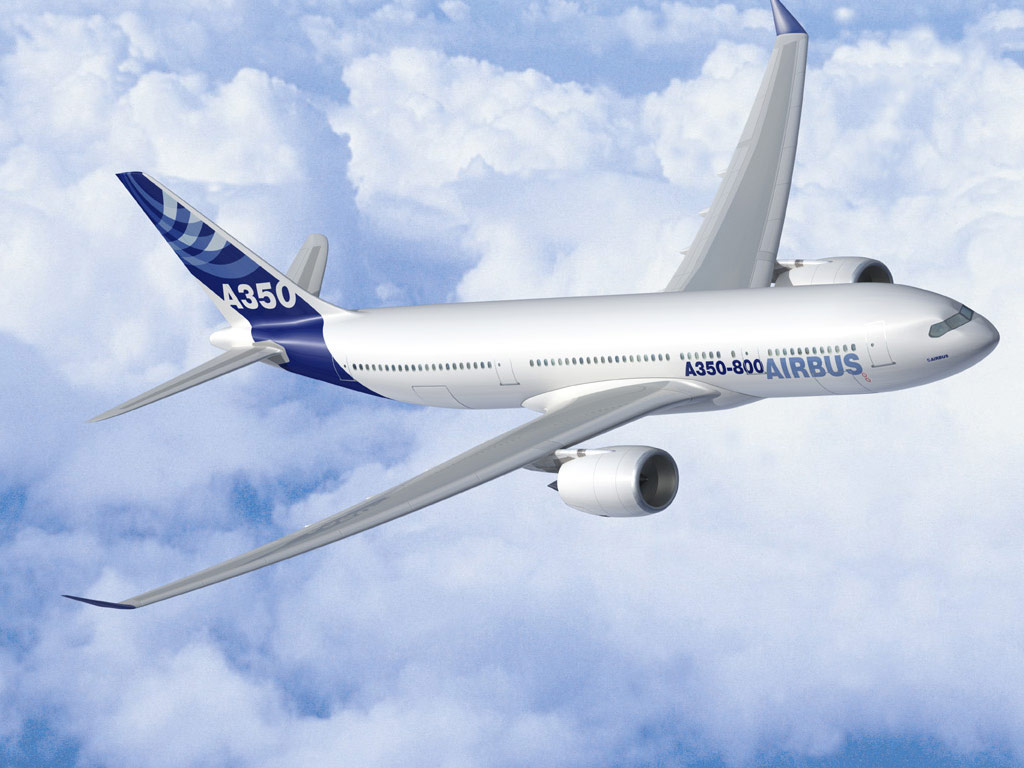
\includegraphics[height=50mm]{Figures/Airbus_A350.jpg}

% Title, author and degree
\vspace{1.0cm}
{\FontLb Thesis Title} \\ % <<<<< EDIT TITLE
%\vspace{0.2cm}
%{\FontMn Subtitle (optional)} \\
%\vspace{1.9cm}
\vspace{2.6cm}
{\FontMb Candidate João} \\ % <<<<< EDIT NAME
\vspace{2.0cm}
{\FontSn \coverThesis} \\
\vspace{0.3cm}
{\FontLb Aerospace Engineering} \\ % <<<<< EDIT COURSE
\vspace{1.0cm}
{\FontSn %
\begin{tabular}{ll}
 \coverSupervisors: & Prof. Full Name 1 \\ % <<<<< EDIT NAME
                    & Dr. Full Name 2    % <<<<< EDIT NAME
\end{tabular} } \\
\vspace{1.0cm}
{\FontMb \coverExaminationCommittee} \\
\vspace{0.3cm}
{\FontSn %
\begin{tabular}{c}
\coverChairperson:     Prof. Full Name 1  \\ % <<<<< EDIT NAME
\coverSupervisor:      Prof. Full Name 2  \\ % <<<<< EDIT NAME
\coverMemberCommittee: Prof. Full Name 3     % <<<<< EDIT NAME
\end{tabular} } \\
\vspace{1.5cm}
{\FontMb Month Year} \\ % <<<<< EDIT DATE (corresponds to date of oral examination)
%
\end{center}
 % file "Thesis_FrontCover.tex"
\cleardoublepage

% ----------------------------------------------------------------------
% Dedication page (optional)
% ----------------------------------------------------------------------
%%%%%%%%%%%%%%%%%%%%%%%%%%%%%%%%%%%%%%%%%%%%%%%%%%%%%%%%%%%%%%%%%%%%%%%%
%                                                                      %
%     File: Thesis_Dedication.tex                                      %
%     Tex Master: Thesis.tex                                           %
%                                                                      %
%     Author: Andre C. Marta                                           %
%     Last modified :  2 Jul 2015                                      %
%                                                                      %
%%%%%%%%%%%%%%%%%%%%%%%%%%%%%%%%%%%%%%%%%%%%%%%%%%%%%%%%%%%%%%%%%%%%%%%%

\null\vskip5cm%
\begin{flushright}
     Dedicate to someone special ...
\end{flushright}
\vfill\newpage

 % file "Thesis_Dedication.tex"
\cleardoublepage

% ----------------------------------------------------------------------
% Declaration page (mandatory)
% ----------------------------------------------------------------------
%%%%%%%%%%%%%%%%%%%%%%%%%%%%%%%%%%%%%%%%%%%%%%%%%%%%%%%%%%%%%%%%%%%%%%%%
%                                                                      %
%     File: Thesis_Declaration.tex                                     %
%     Tex Master: Thesis.tex                                           %
%                                                                      %
%     Author: Andre C. Marta                                           %
%     Last modified :  29 Jun 2022                                     %
%                                                                      %
%%%%%%%%%%%%%%%%%%%%%%%%%%%%%%%%%%%%%%%%%%%%%%%%%%%%%%%%%%%%%%%%%%%%%%%%

\null\vskip5cm%
\begin{flushleft}
	\declarationTitle \\
	\declarationText
\end{flushleft}
\vfill\newpage

 % file "Thesis_Declaration.tex"
\cleardoublepage

% ----------------------------------------------------------------------
%  Acknowledgments (optional)
% ----------------------------------------------------------------------
%%%%%%%%%%%%%%%%%%%%%%%%%%%%%%%%%%%%%%%%%%%%%%%%%%%%%%%%%%%%%%%%%%%%%%%%
%                                                                      %
%     File: Thesis_Acknowledgments.tex                                 %
%     Tex Master: Thesis.tex                                           %
%                                                                      %
%     Author: Andre C. Marta                                           %
%     Last modified :  2 Jul 2015                                      %
%                                                                      %
%%%%%%%%%%%%%%%%%%%%%%%%%%%%%%%%%%%%%%%%%%%%%%%%%%%%%%%%%%%%%%%%%%%%%%%%

\section*{\acknowledgments}

% Add entry in the table of contents as section
\addcontentsline{toc}{section}{\acknowledgments}

A few words about the university, financial support, research advisor, dissertation readers, faculty or other professors, lab mates, other friends and family...
 % file "Thesis_Acknowledgements.tex"
\cleardoublepage

% ----------------------------------------------------------------------
%  Abstract (both in English and Portuguese)
% ----------------------------------------------------------------------
%%%%%%%%%%%%%%%%%%%%%%%%%%%%%%%%%%%%%%%%%%%%%%%%%%%%%%%%%%%%%%%%%%%%%%%%
%                                                                      %
%     File: Thesis_Resumo.tex                                          %
%     Tex Master: Thesis.tex                                           %
%                                                                      %
%     Author: Andre C. Marta                                           %
%     Last modified :  4 Mar 2024                                      %
%                                                                      %
%%%%%%%%%%%%%%%%%%%%%%%%%%%%%%%%%%%%%%%%%%%%%%%%%%%%%%%%%%%%%%%%%%%%%%%%

\section*{Resumo}

% Add entry in the table of contents as section
\addcontentsline{toc}{section}{Resumo}

Inserir o resumo em Portugu\^{e}s aqui com um máximo de 250 palavras e acompanhado de 4 a 6 palavras-chave.

\vfill

\textbf{\Large Palavras-chave:} palavra-chave1, palavra-chave2, palavra-chave3,...

   % file "Thesis_Resumo.tex"
\cleardoublepage

%%%%%%%%%%%%%%%%%%%%%%%%%%%%%%%%%%%%%%%%%%%%%%%%%%%%%%%%%%%%%%%%%%%%%%%%
%                                                                      %
%     File: Thesis_Abstract.tex                                        %
%     Tex Master: Thesis.tex                                           %
%                                                                      %
%     Author: Andre C. Marta                                           %
%     Last modified :  4 Mar 2024                                      %
%                                                                      %
%%%%%%%%%%%%%%%%%%%%%%%%%%%%%%%%%%%%%%%%%%%%%%%%%%%%%%%%%%%%%%%%%%%%%%%%

\section*{Abstract}

% Add entry in the table of contents as section
\addcontentsline{toc}{section}{Abstract}

Insert your abstract here with a maximum of 250 words, followed by 4 to 6 keywords.

\vfill

\textbf{\Large Keywords:} keyword1, keyword2, keyword3,...

 % file "Thesis_Abstract.tex"
\cleardoublepage

% ----------------------------------------------------------------------
%  Table of contents, list of tables, list of figures and nomenclature
% ----------------------------------------------------------------------

% Table of contents
%
\tableofcontents
\cleardoublepage 

% List of tables
%
% Add entry in the table of contents as section
\phantomsection
\addcontentsline{toc}{section}{\listtablename}
% Generate list
\listoftables
\cleardoublepage 

% List of figures
%
% Add entry in the table of contents as section
\phantomsection
\addcontentsline{toc}{section}{\listfigurename}
% Generate list
\listoffigures
\cleardoublepage 

% Nomenclature
%
% Add entry in the table of contents as section
\phantomsection
\addcontentsline{toc}{section}{\nomname}
% Insert nomenclature section produced by \makenomenclature
\printnomenclature
\cleardoublepage

% Glossary
%
% Add entry in the table of contents as section
\phantomsection
\addcontentsline{toc}{section}{\acronymname}
% Insert glossary section produced by \makeglossaries
\printglossary[type=\acronymtype,title=\acronymname, toctitle=\acronymname]
%\printglossary[type=\acronymtype,style=long,title=\acronymname, toctitle=\acronymname]
\cleardoublepage

% Set arabic numbering (1,2,...) after preface
%
\setcounter{page}{1}
\pagenumbering{arabic}

% ----------------------------------------------------------------------
%  Chapters
% ----------------------------------------------------------------------

%%%%%%%%%%%%%%%%%%%%%%%%%%%%%%%%%%%%%%%%%%%%%%%%%%%%%%%%%%%%%%%%%%%%%%%%
%                                                                      %
%     File: Thesis_Introduction.tex                                    %
%     Tex Master: Thesis.tex                                           %
%                                                                      %
%     Author: Andre C. Marta                                           %
%     Last modified :  4 Mar 2024                                      %
%                                                                      %
%%%%%%%%%%%%%%%%%%%%%%%%%%%%%%%%%%%%%%%%%%%%%%%%%%%%%%%%%%%%%%%%%%%%%%%%

\chapter{Introduction}
\label{chapter:introduction}


%%%%%%%%%%%%%%%%%%%%%%%%%%%%%%%%%%%%%%%%%%%%%%%%%%%%%%%%%%%%%%%%%%%%%%%%
\section{Motivation}
\label{section:motivation}

testeee

teste 123456789 00

%%%%%%%%%%%%%%%%%%%%%%%%%%%%%%%%%%%%%%%%%%%%%%%%%%%%%%%%%%%%%%%%%%%%%%%%
\section{Topic Overview}
\label{section:topic_overview}

When it comes to helicopter emergency manoeuvres, autorotation is one of the most important skills that pilots use in the event of a failure of the engine \cite{federal_aviation_administration_helicopter_2021}. This method uses a controlled fall that starts with reducing the collective pitch control. Then it uses upward airflow to provide lift, maintain rotation of the rotor blade, and postpone descent. To maintain control throughout the manoeuvre, the pilots adjust the direction and attitude of the helicopter using cyclic control. The pilot performs a flare, further slowing the descent velocity as the helicopter gets closer to Earth by lowering the collective a little. Because auto-rotation is a skill that is acquired via extensive training, it is a dependable way for pilots to land safely in the event of unplanned power outages, which greatly enhances aviation safety in general.

Comparably, more sophisticated technologies have replaced conventional parachute systems in the investigation of recovery systems in space missions. In particular, the \gls{vtc} recovery system poses development, installation, and cost issues despite providing precise control over the descent speed and trajectory \cite{federal_aviation_administration_helicopter_2021}. In light of these factors, a novel method using a rotary wing recovery system under autorotation effect appears in light of these factors. This method has been developed for years, but it has not been put into practice, probably because of financial and/or technological limitations.


By combining the benefits of controlled thrust vector and parachute systems, the suggested rotary wing recovery system promises maneuverability, economic feasibility, and reusability. Using autorotation, similar in a helicopter, the technology ensures a safe and controlled landing. This recovery approach is still a promising and unexplored area in the rapidly changing field of technical developments, and further research is necessary to fully realise its potential. The complex properties of the system and the phenomenon of auto-rotation serve as the main topics of current research.


%%%%%%%%%%%%%%%%%%%%%%%%%%%%%%%%%%%%%%%%%%%%%%%%%%%%%%%%%%%%%%%%%%%%%%%%
\section{Objectives}
\label{section:objectives}


Previous studies have been conducted to explore the use of auto-rotation phenomena as a recovery method for spacecraft vehicles. In this subject \gls{armada} project \cite{noauthor_armada_nodate} is a key publication once it was done by major players . Also, many studies  as \cite{steiner_rotary_nodate} take the first step by using \gls{armada} vehicle concepts for its studies.For instance, the master's thesis by Marques \cite{marques_design_2024} investigated the phenomena in axial flight, demonstrating through simulations that the system functions as expected. However, certain aerodynamic considerations and assumptions were made, as well as in other works as \textcolor{blue}{meter aqui mais referências de outros artigos com referencias a modelos simplificados}

The proposed works aims to dig deep into the concept, trying to create a more sophisticated and fidelity model for rotary wings under autorotation effect and increase the inside knowledge of the subject. So, for emproving and achieve the main goals, several other intermidiate objectives should be define. First objective is to conduct an literature review shall be made in order to understand concept's limitations and linking those limitations with modeling and wind tunnel tests limitations.

As second, a 6-D0F dynamic model is developed along with the \gls{bet} for the rotary wing aerodynamic analysis. This parts, highlight all the necessary mathematical tools to simulate and 

The third step is to build an simple Matlab simuator which 


%%%%%%%%%%%%%%%%%%%%%%%%%%%%%%%%%%%%%%%%%%%%%%%%%%%%%%%%%%%%%%%%%%%%%%%%
\section{Thesis Outline}
\label{section:outline}

The document is divided into three main parts which will focus on the three key points of this thesis: Literature Review, 6-DOF BET Model, and Simulations

The chapter \ref{chapter:literaturereview} reviews the state of the rocket recovery today, examining a range of pruposed models and project and comparing them with other system from simple parachutes to sophisticated propulsive landing systems. It starts from understading the major opportunities and the interest of new technologies in aerospace industrie, on section \ref{section:spacerace_reusability}. On the other hand, section \ref{section:autorotation_vehicles} focus on previous projects which try to use rotary-wing under the phenomena of autorotation for spacecraft recovery. In this section some topics and presented as vehicle concepts, mathemativcal models and wind tunnel test, and successes and difficulties of this projet. Focusing on autorotation, a crucial idea in aerodynamics, section \ref{section:autorotation_phenomena} examines the fundamental mathematical models behind it. The key point is to understand \textcolor{blue}{explicar}


Chapter \ref{chapter:mathematical_model} \textcolor{blue}{explicar} % file "Thesis_Introduction.tex"
\clearpage

%%%%%%%%%%%%%%%%%%%%%%%%%%%%%%%%%%%%%%%%%%%%%%%%%%%%%%%%%%%%%%%%%%%%%%%%
%                                                                      %
%     File: Thesis_Background.tex                                      %
%     Tex Master: Thesis.tex                                           %
%                                                                      %
%     Author: Andre C. Marta                                           %
%     Last modified:  4 Mar 2024                                       %
%                                                                      %
%%%%%%%%%%%%%%%%%%%%%%%%%%%%%%%%%%%%%%%%%%%%%%%%%%%%%%%%%%%%%%%%%%%%%%%%

\chapter{Literature Review}
\label{chapter:literaturereview}


%%%%%%%%%%%%%%%%%%%%%%%%%%%%%%%%%%%%%%%%%%%%%%%%%%%%%%%%%%%%%%%%%%%%%%%%
\section{Space Race and Vehicles Reusability}
\label{section:spacerace_reusability}

\textcolor{blue}{Procura pelo espaço}

\textcolor{blue}{Baixo custo de missões, reutilização de estágios}

\textcolor{blue}{Problema de reentrada}

\textcolor{blue}{Novas tecnologias - falar aqui das tecnologias atuais}

%%%%%%%%%%%%%%%%%%%%%%%%%%%%%%%%%%%%%%%%%%%%%%%%%%%%%%%%%%%%%%%%%%%%%%%%
\section{Autorotation for Space Vehicles}
\label{section:autorotation_vehicles}

Using an unpowered rotary wind as an aerodynamic decelerator for spacecraft recovery from a space mission is not a new concept. More than 80 years ago, the first studies were performed, but rapidly the concepts lost interest \textcolor{purple}{encontrar esta referência}. Years after it gained new enthusiasts and some recent projects were published. This section assesses the evolution of the use of Autorotation for Spacecraft.

\subsection{Rotary Wing Recovery System In the Early Ages of Space Exploration}

Over the years some studies have been published focusing on using rotary wings as a concept for vehicle recovery. Ricardo A. Diaz-Silva in \cite{diaz-silva_rotary_2013}, states that early concepts date 1947, when Igor Bensen, from the General Electric Co, published a report titled \textit{Development of Rotochute Rotary Wing Air Brake}. In its work, Bensen developed a device known as Rotochute (fig \ref{fig:rotochute_prototype}) which is a result of merging two keywords: rotor and parachute. The main objective of this device was to develop an aerodynamic decelerator for high-altitude rockets. This device was at the time studied at a supersonic wind tunnel to understand reentry effects. 

\begin{figure}[!htb]
    \centering
    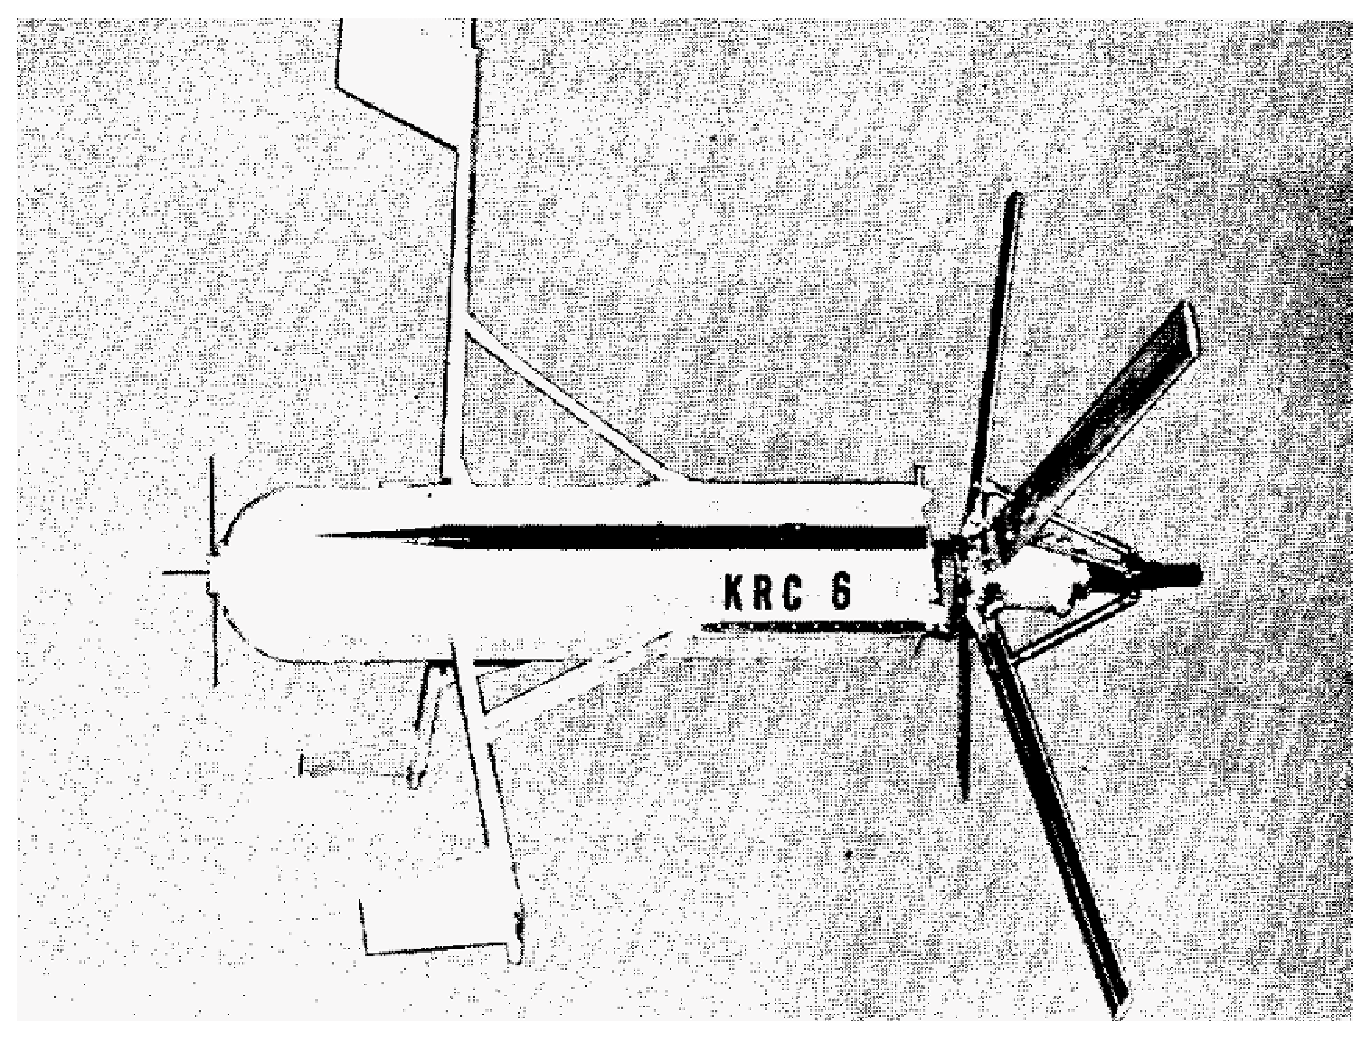
\includegraphics[width=8cm]{Figures/literature_review/rotochute_prototype.eps}
    \caption{KRC-6 Rotochute Flight Test Vehicle}
    \label{fig:rotochute_prototype}
\end{figure}

Also, Kaman Corporation got involved in the rotochute design in the 50s decade and the \gls{nasa} spent some attention studying the proposed system in the 60's, never putting it into practice once all Apollo Missions \cite{noauthor_apollo_nodate} were accomplished by recovering the crew capsule with parachutes landing on the ocean. Important authors in this decade working on the topic, cited in \cite{diaz-silva_rotary_2013}, were Rodney Wernicke from the Bell Helicopter Company, 1957, Justin J. Barzda from Kaman Corporation, 1964, and M. Kretz from the Giravions Dorand Co. in France, 1966. These authors made a substantial original contribution to the area, it is important to comprehend the main ideas of this system by providing a brief overview of their work.

Wernicke published \textit{Preliminary Tests of Model Spacecraft Rotor Landing System} where a three-bladed model was used as able to reduce the vehicle descent axial velocity from supersonic regime to subsonic glide. In its work, Wernicke studied the influence of collective pitch on the model's performance.

On the other hand, Barzda published \textit{Rotor for Recovery} were fixed and telescoping span blades, rotor diameters ranging from 0.3 to 7.3 meters, payloads 2.7 to 408 kg, and rates of descent as low as 6 m/s were points of experimental tests. Barzda did the experimental investigation of deployment from jet aircraft and from a cannon-fired flare shell at  Mach numbers 0.98 and 1.2, respectively. From this investigation, drag and lift coefficients, glide ratios, and cyclic and collective flare performance were crucial results, necessary for the advancement of the concept.

\textit{Space Rotor: A European Project for Recovery of Heavy Launch Vehicles} was published by Kretz and registered a patent. His design aimed to help spacecraft return from orbit by using rotors that could be deployed before re-entry. The system offered benefits like better flight stability, longer range, and precise, soft landings, making reusable launch vehicles possible.

From a historical perspective, Diaz-Silva \cite{diaz-silva_rotary_2013} also makes reference to a Sovietic interest in this system for its Soyuz capsule recovery system, but no references can be found.

\subsection{Recent Projects}
\label{sec:recent_projects}


In recent years, new developments have been published about using rotary wings for recovery space vehicles. The publications show completely different results from the early concepts once the computation technologies have also evolved over the years. It allows researchers to gain deep knowledge of the autorotation phenomena throw computational simulations. Also, conceptual model vehicles were possible to be built with onboard computers to get data from experimental flights due to electronics development.

\subsubsection{\gls{armada}}

A fundamental state-of-the-art project was started to be developed in 2008  by the \gls{esa}, GMV, the University of Bologna and the European Aeronautic \gls{EADS}. The so-called \gls{armada} project \cite{noauthor_armada_nodate} is an \gls{edls}. Its relevance in the field is significant once many other projects were published and taken as reference \gls{armada} project. 

 In the proposed system of \gls{armada} (figure \ref{fig:armada_concept}) a rotor is connected to a conventional helicopter control system, which in turn is mounted on the structure that supports the payload. The deployment process occurs in several stages. Initially, body flaps extend to stabilize the vehicle during deployment. Following this, the rotor blades are deployed using a cable to minimize stress on the joints. 

\begin{figure}[!htb]
    \centering
    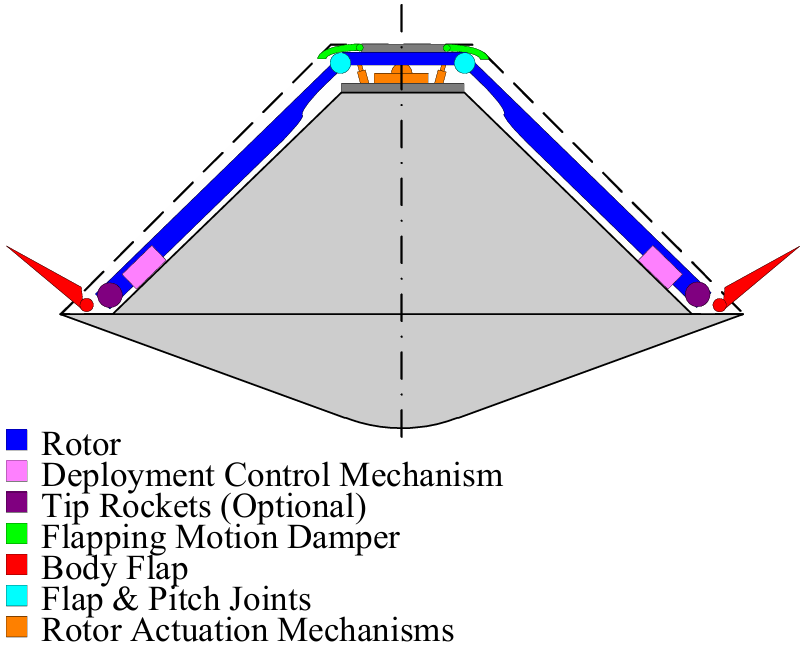
\includegraphics[width=8cm]{Figures/literature_review/armada_concept_vehicle.png}
    \caption{ARMADA Autorotation system concept, from \cite{noauthor_armada_nodate} }
    \label{fig:armada_concept}
\end{figure}

During the deployment, the blades are set to a zero-lift configuration to prevent rotation, with an additional braking system on the rotor shaft ensuring no movement. Once the blades are fully deployed, the retention cables are released, the rotor brake is disengaged, and the collective pitch of the blades is adjusted to allow the rotor to spin. As the lander crosses a predetermined Mach number, centrifugal force extends the telescopic blades, which were initially held in a retracted position by a cable. From this point, the lander descends in its fully deployed state, reaching an equilibrium descent velocity. Just before landing, a flare manoeuvre is executed to further reduce both vertical and horizontal velocities for a safe touchdown.

In \cite{noauthor_armada_nodate}, the deployment phase is further addressed by considering different types of rotor deployment systems. Using a single-piece blade rotor is small and suitable for thicker atmospheres, while a telescopic blade rotor features extendable sections for easy deployment using internal cables. Inflatable blade rotors are lightweight and compact but store less kinetic energy, limiting their manoeuvrability. Foldable blade rotors require precise locking mechanisms to ensure structural stiffness and flexible blade rotors are stabilized through reefing lines, stiffeners, or centrifugal forces in their deployed state. To achieve the best deployment, the authors state that "Any deployment system that can modify the blade length in-flight is highly desirable since this allows an easy method of reefing.", proposing more suitable telescopic blades.

\gls{armada} concepts performance is done using simulations and wind tunnel experiments. Starting with the software tools, figure \ref{fig:armada_software}, uses a divide and conquer approach in which a Performance Database (PD) and an Integrated Parametric Design  Tool (IPDT). To resume how it works, de PD is in simple words a tabe with rotor parameters under specific conditions and de IPDT is interface sheets that interact with the database.

\begin{figure}[!htb]
    \centering
    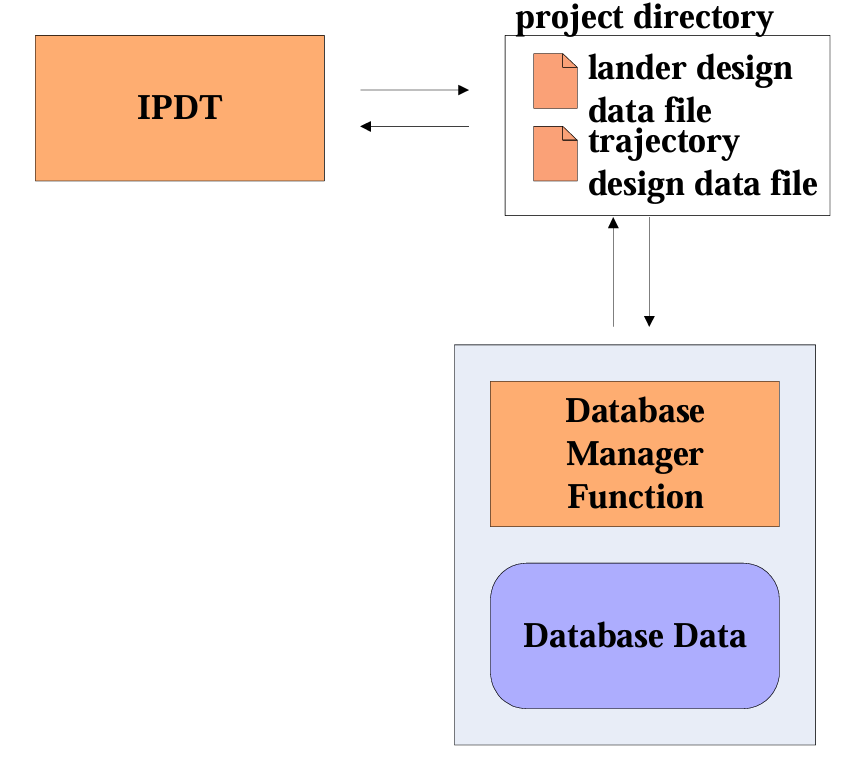
\includegraphics[width=6cm]{Figures/literature_review/armada_software.png}
    \caption{ARMADA concept software, from \cite{noauthor_armada_nodate} }
    \label{fig:armada_software}
\end{figure}

For the experimental tests, a small-scale model, presented in figure \ref{fig:armada_windtunnel} is used. For the supersonic deployment model, figure \ref{fig:armada_supersonic_model}, the S-1 supersonic/transonic wind tunnel 
at Von Karman Institute of Fluid Dynamics was used to test it to Mach number up to 2. For the subsonic regime, the model is tested in the wind tunnel of the Applied Aerodynamic Laboratory of the University of Bologna.

\begin{figure}[!htb]
    \centering
    \subfloat[Supersonic deployment model\label{fig:armada_supersonic_model}]{
        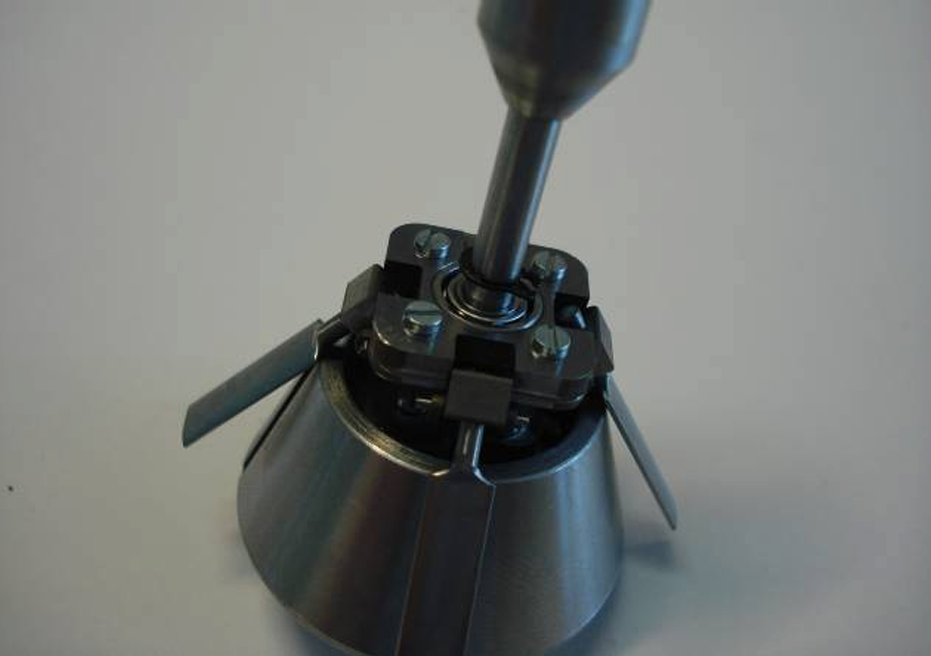
\includegraphics[height=6cm]{Figures/literature_review/armada_supersonic_model.png}
    }\hfill
    \subfloat[Subsonic reefing model\label{fig:aircraft2}]{
        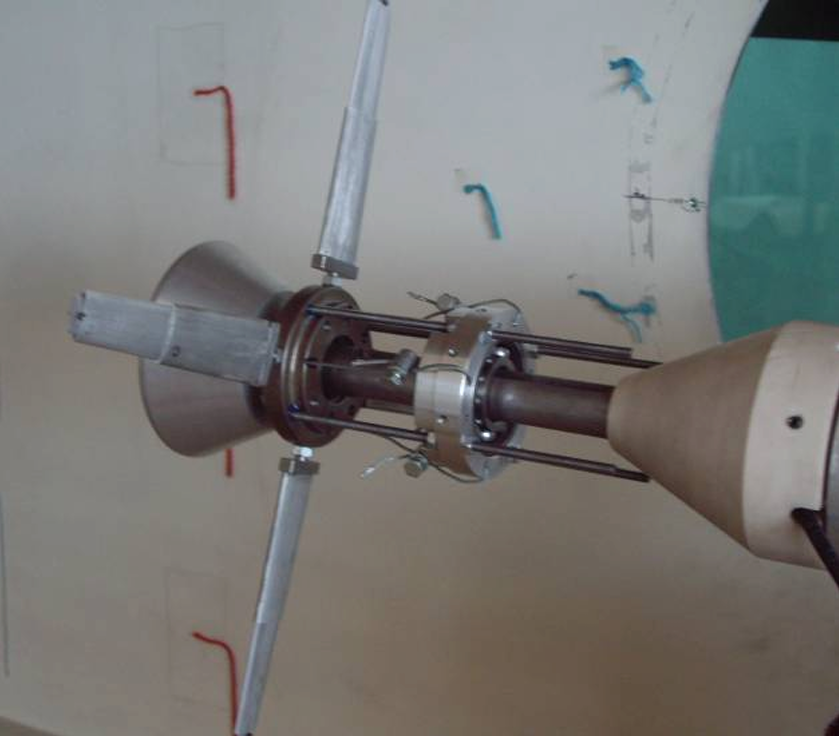
\includegraphics[height=6cm]{Figures/literature_review/armada_subsonic_model.png}
    }
    \caption{ARMADA concepts under different fight conditions}
    \label{fig:armada_windtunnel}
\end{figure}

As results of the study \cite{noauthor_armada_nodate}, show an equilibrium descent velocity that can be obtained with the type of design presented is about 30-40 $m/s$ and was found that this terminal velocity cannot be reduced by increasing the rotor size, and the mass of the rotor itself becomes an important contributor to the overall mass of the vehicle. About this point an essential remark is made:  the mass of the recovery system remains attached to the vehicle, but in traditional systems some mass gets ejected (parachutes) or burnt (propellant). In terms of aerodynamic performance, the distinction between stalled and unstalled operation is evident in the rotor drag coefficient and descent velocity. In installed conditions, the rotor drag coefficient ranges from 1 to 1.25, with a descent velocity of approximately 31 $m/s$. Conversely, when stalled, the rotor drag coefficient drops to around 0.25, and the descent velocity increases significantly to about 80 $m/s$. Furthermore, \gls{armada} faces mechanical challenges, including rotor mass, complexity, descent velocity, and vibration issues. Future solutions may involve improved materials and structures, integrated control systems, and the consideration of additional braking mechanisms.

ARMADA's performance does not justify short-term adoption compared to traditional \gls{edls}. Further research on these approaches is necessary. Overall, ARMADA presents a promising alternative for EDL systems on Earth, Venus, or Titan in the medium to long term.



\subsubsection{Hummingbird}

Further investigation takes to another conceptual project. An undergraduate research project called Project Hummingbird \cite{maurer_project_nodate} aims to launch and recover a sounding rocket with a safe landing achieved by a rotor recovery mechanism. The effort aims to introduce a novel approach to booster recovery that minimizes fuel requirements, streamlines the system, and lowers launch costs.

With foldable rotor blades and an internally stored rotor hub, the system is designed to launch to a height of 2,700 meters. A little parachute will pop out of the nose cone's tip at apogee, allowing the rocket to be oriented with its nose facing upwards. The nose cone will separate in its entirety upon correct alignment. The rotor blades will then immediately deploy and start to revolve on their own, slowing the rocket's descent speed. The rotor will execute a flare movement as the rocket gets closer to the ground to guarantee a safe landing. There will be a flight computer monitoring the rocket's direction and fall. If the rotor blades fail to sufficiently slow down the drop, an emergency parachute will deploy.

\begin{figure}[!htb]
    \centering
    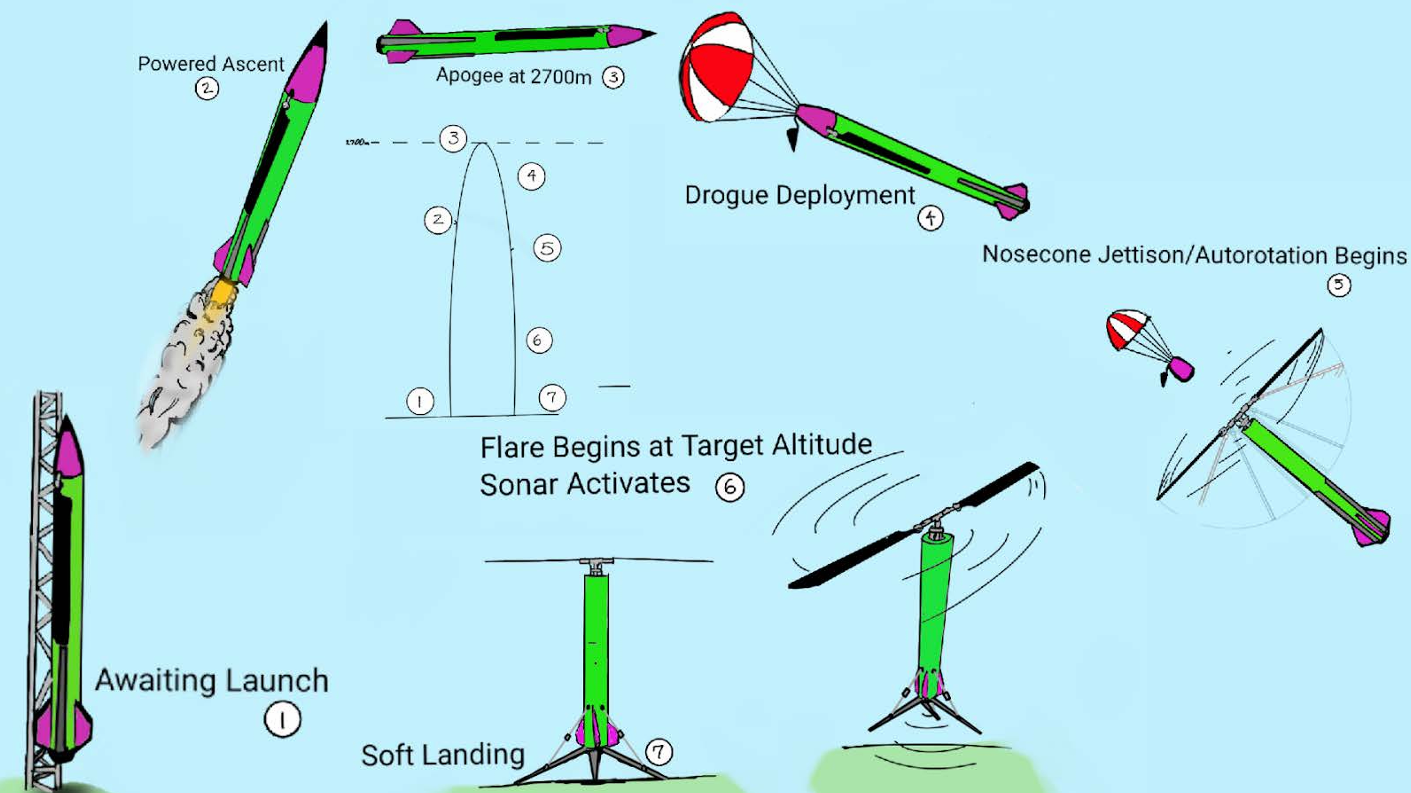
\includegraphics[width=10cm]{Figures/literature_review/Hummingbird_operation.png}
    \caption{Concept of Operation of Project Hummingbird, from \cite{maurer_project_nodate}}
    \label{fig:Hummingbird_operation}
\end{figure}

This project demonstrates an alternative application of rotary wings as a recovery system and introduces a useful hybrid system that combines parachutes and rotary wings. This combination could be crucial if the vehicle is not in the correct position during rotor deployment. Additionally, higher velocities during the deployment phase may result in increased structural stresses, as noted in \cite{noauthor_armada_nodate}.

\subsubsection{DEADALUS}

Riegler et al. developed a prototype \cite{riegler_daedalus_2018} aiming for Earth atmospheric research but also for other \gls{leo} missions. In this work, the authors state that new and safe technologies are needed in the field, proposing a self-stabilizing, free-falling unit, capable of measuring and distributing atmospheric data during descension \cite{riegler_daedalus_2018}. For accomplished the teams goal's, they started by develop the rocket prototype called REXUS, presented in figure 3. 


\begin{figure}[!htb]
    \centering
    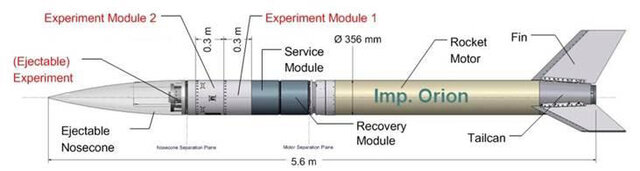
\includegraphics[width=10cm]{Figures/literature_review/REXUS-Rocket-composition_W640.jpg}
    \caption{REXUS Rocket composition, from \cite{riegler_daedalus_2018}}
    \label{fig:rexus_rocket}
\end{figure}

On the REXUS prototype a set o  \gls{ffu} so called SpaceSeeds, are placed inside the REXUS cone, figure \ref{fig:ffu_rexus_inside} and will be injected once the rocket reaches its apogee. This SpaceSeeds are the intereste key point of DEADALUS project on the scope of the use of rotary wings under autorotation phenomena as a recovery system for spacecraft. Figure \ref{fig:ffu_rexus_model} presents a SpaceSeed prototype is presented with four-bladed rotor and a conical main body.



\begin{figure}[!htb]
    \centering
    \subfloat[SpaceSeeds placement inside REXUS's cone, from \cite{noauthor_daedalus_nodate}\label{fig:ffu_rexus_inside}]{
        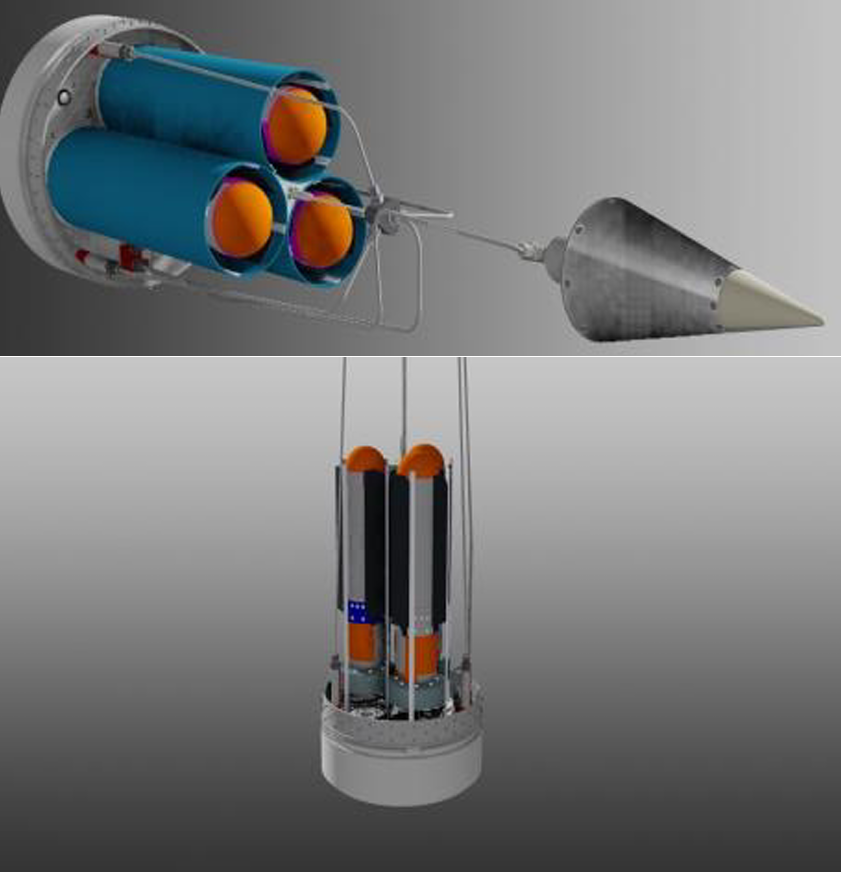
\includegraphics[height=7cm]{Figures/literature_review/ffu_rexus.png}
    }\hfill
    \subfloat[SpaceSeed protoype, from \cite{riegler_project_nodate}\label{fig:ffu_rexus_model}]{
        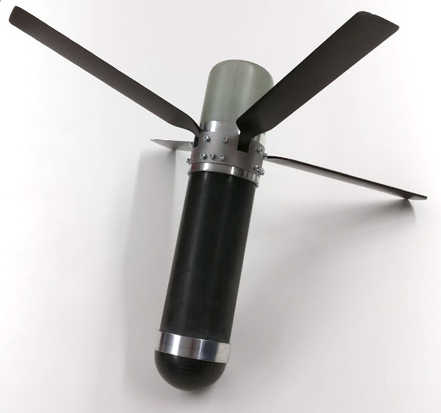
\includegraphics[height=7cm]{Figures/literature_review/space_seed_prototype.png}
    }
    \caption{\gls{ffu} SpaceSeeds used in DEADALUS project}
    \label{fig:daedalus_ffu}
\end{figure}

The development and construction of the space are further presented by Riegler et al. in \cite{riegler_project_nodate}. In this study, the authors explain in better detail the aerodynamic characteristics and software and telemetry information and electronics and its \gls{orbc}. Using the paper words, the \gls{orbc} is the interface between the \gls{rxsm} and the SpaceSeeds, so it is important to refer to it. 

Another important aspect of the project is the mechanical setup. Although it is not the main subject of this study, it is important to highlight the necessity of other components in \cite{riegler_project_nodate} technology. Related to this work two key points are presented: the deployment mechanism which is a crucial aspect of the project once it is necessary to separate the SpaceSeeds from the launcher; the second important point is the wings folding mechanism. The latest mechanical components are not a key point for this study, but it is important to take into consideration, that for spacecraft recovery the blades must be kept inside the vehicle during the launch phase. The blades should only open, unfold or any other way of deploy during the descent phase.

For the mechanical setup, the authors found some mechanical challenges that one must take into consideration: flight loads, especially in the transonic regime, minimum weight, volumetric constraints, natural aerodynamic stability, antenna positioning, radio translucent materials at corresponding areas and landing shock loads.

Finally and more important, is the flight tests. In \cite{riegler_project_nodate} the authors presented a set of different simulation and real flight tests showing good accuracy from computational model and real-flight data. A deeper look at this data is taken in section \textcolor{blue}{meter aqui referência à secção de validação} in which the data is used to validate the computational model presented in this.

From the same authors \cite{mehringer_suborbital_2022} and \cite{bergmann_daedalus_2024} are two more recent publications about the DEADALUS project, in this case, the second version. In thiese papers, some improvements are made to the setup but no available data is presented for comparison.


\subsection{Why using rotary wings for space vehicle recovery?}

\textcolor{blue}{comparação}

To understand why using a rotary wing is a key advantage in space exploration, one can get back to Barzda's work \cite{barzda_rotors_1964} where it is answered. This analysis is mainly done by connecting an already known application of autorotation: helicopters autorotation mandatory manoeuvre in case of power losses \cite{federal_aviation_administration_helicopter_2021}. As helicopters, this is a weatherproof system that can perform under icing or stormy conditions. Another important advantage is the fast and precise deployment over a wide range of speeds. Retardation force builds up rapidly when body orientation is adequate. This allows for recovery, for example, the launcher, when it is necessary to abort the mission in the middle flight to save human lives or payload. A rotary wing is a controllable system, meaning that the pilot can use flight controls to control the vehicle trajectory and rate of descent \cite{federal_aviation_administration_helicopter_2021}. This is an important feature of this system once it is possible to make a safe landing at the intended landing site.

Also over the traditional, parachute, and nowadays in-development technology, \gls{vtc}, using rotary wing under autorotarion phenomena has some advantages. In section \ref{section:spacerace_reusability} a variety of new technologies were presented, however, there is no interest in comparison once none of them were put into practice. In \cite{marques_rocket_2022}, present a table comparing four different recovery technologies showing an outstanding advantage over the parachute and a good advantage over \gls{vtc}. Over the parachute system, cost and weight are the major drawbacks. Relatively to \gls{vtc}, the rotary wings system presents the possibility of controlled gliding, mission flexibility and a wider range of applications. Another table was presented by Steiner \cite{steiner_rotary_nodate} who also used as a recovery methods comparison criterion the unpowered advantage of the autorotation system. 

%%%%%%%%%%%%%%%%%%%%%%%%%%%%%%%%%%%%%%%%%%%%%%%%%%%%%%%%%%%%%%%%%%%%%%%%
\section{Autorotation Phenomena}
\label{section:autorotation_phenomena}



%%%%%%%%%%%%%%%%%%%%%%%%%%%%%%%%%%%%%%%%%%%%%%%%%%%%%%%%%%%%%%%%%%%%%%%%
\section{State-of-art Overview and Conclusions}
\label{section:state_of_art_conclusions}

 % file "Thesis_Background.tex"
\clearpage

%%%%%%%%%%%%%%%%%%%%%%%%%%%%%%%%%%%%%%%%%%%%%%%%%%%%%%%%%%%%%%%%%%%%%%%%
%                                                                      %
%     File: Thesis_Implementation.tex                                  %
%     Tex Master: Thesis.tex                                           %
%                                                                      %
%     Author: Andre C. Marta                                           %
%     Last modified :  4 Mar 2024                                      %
%                                                                      %
%%%%%%%%%%%%%%%%%%%%%%%%%%%%%%%%%%%%%%%%%%%%%%%%%%%%%%%%%%%%%%%%%%%%%%%%

\chapter{Autorotation Mathematical Model}
\label{chapter:mathematical_model}


%%%%%%%%%%%%%%%%%%%%%%%%%%%%%%%%%%%%%%%%%%%%%%%%%%%%%%%%%%%%%%%%%%%%%%%%
\section{Vehicle Model}
\label{section:model}

When it comes to spacecraft vehicles, a very complex geometry is crucial to achieve a space mission. However, when one looks at different vehicles from old types like the Saturn V to new ones like the Falcon 9, the geometry is similar for the entire vehicle when it is launched. A giant launcher is used to put into orbit a smaller payload. This geometry is still in use and does not show a greater margin in progress in the following years, once one can understand from figure \ref{fig:rocket_models}, where three different vehicles are presented from different companies.

\begin{figure}[!htb]
    \centering
    \subfloat[Ariane 6 \cite{noauthor_european_nodate}\label{fig:ariane_6}]{
        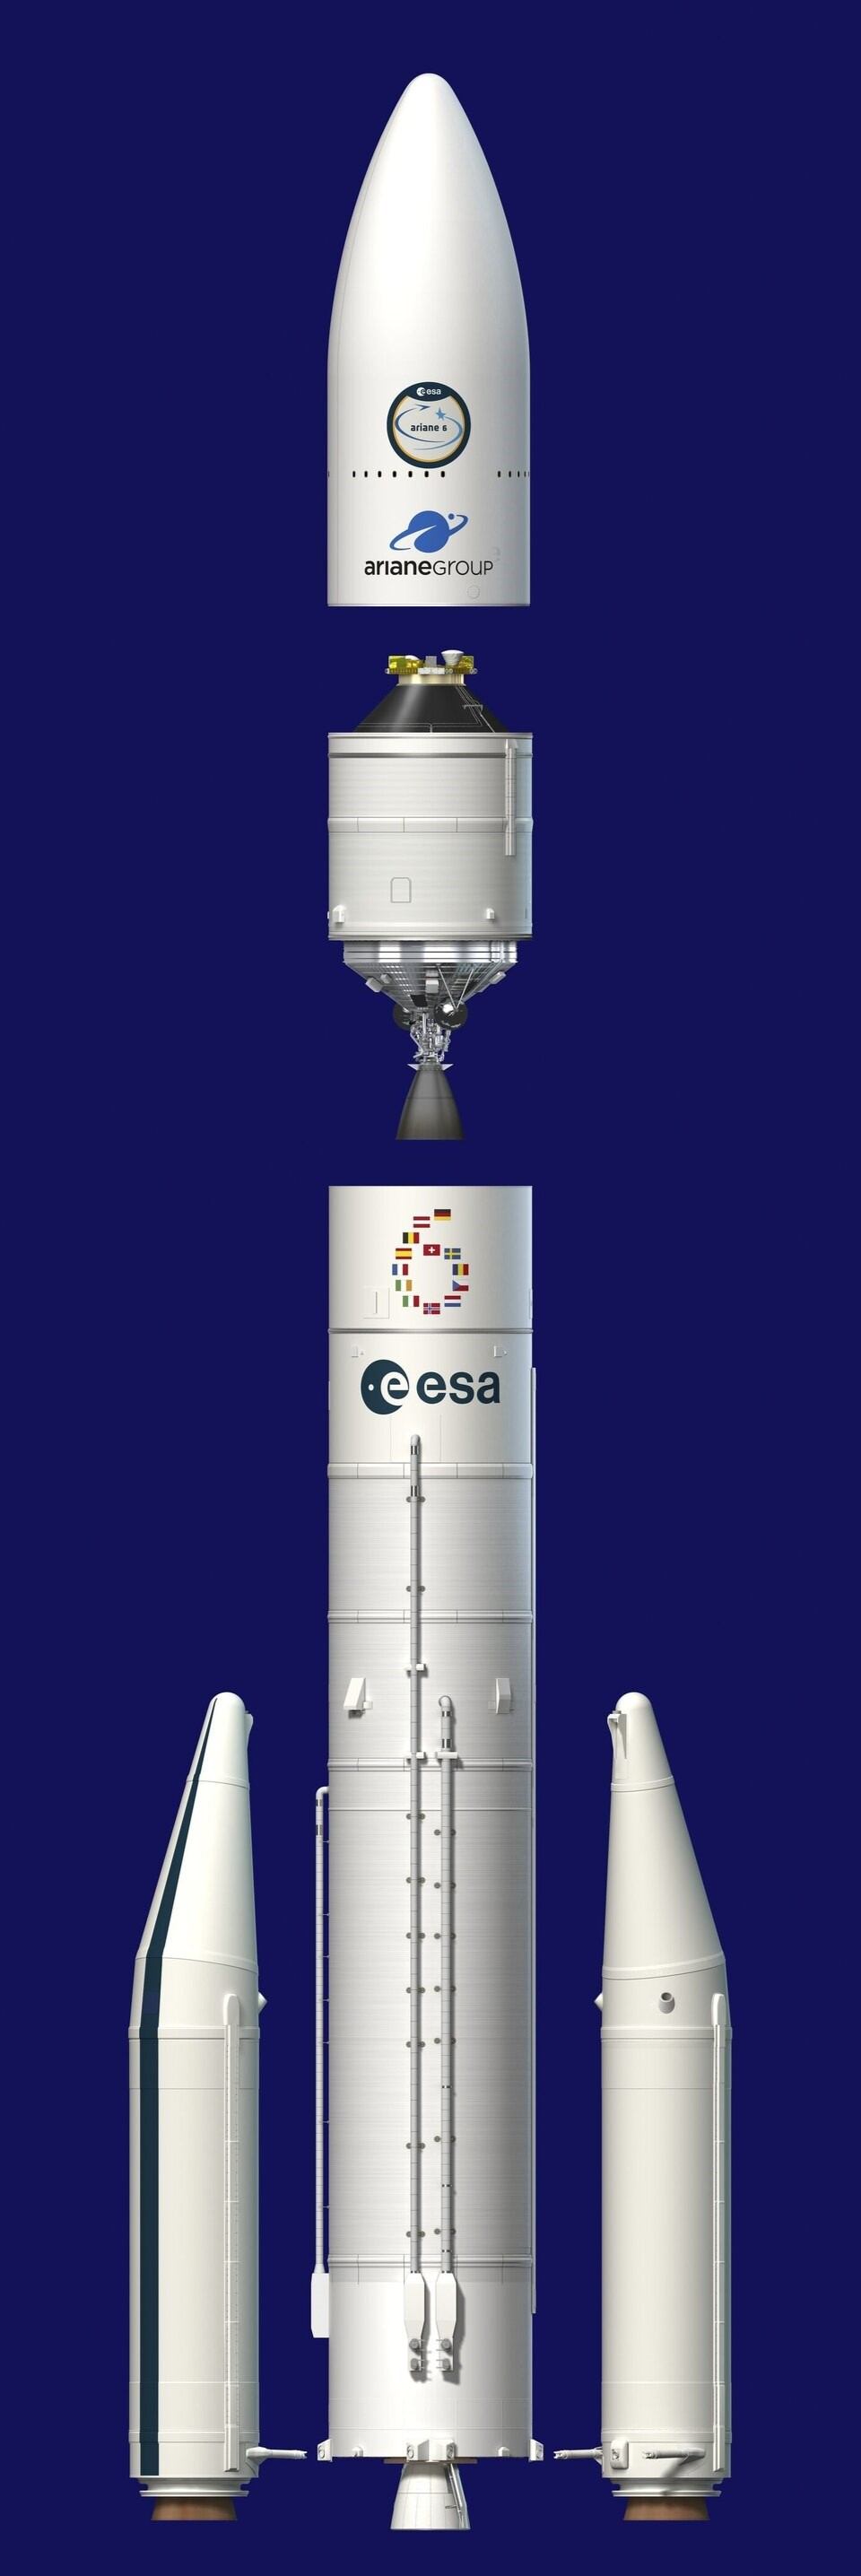
\includegraphics[height=7cm]{Figures/implementation/model/ariane_6.jpg}
    }\hfill
    \subfloat[Falcon 9 \cite{noauthor_spacex_nodate}\label{fig:falcon_9}]{
        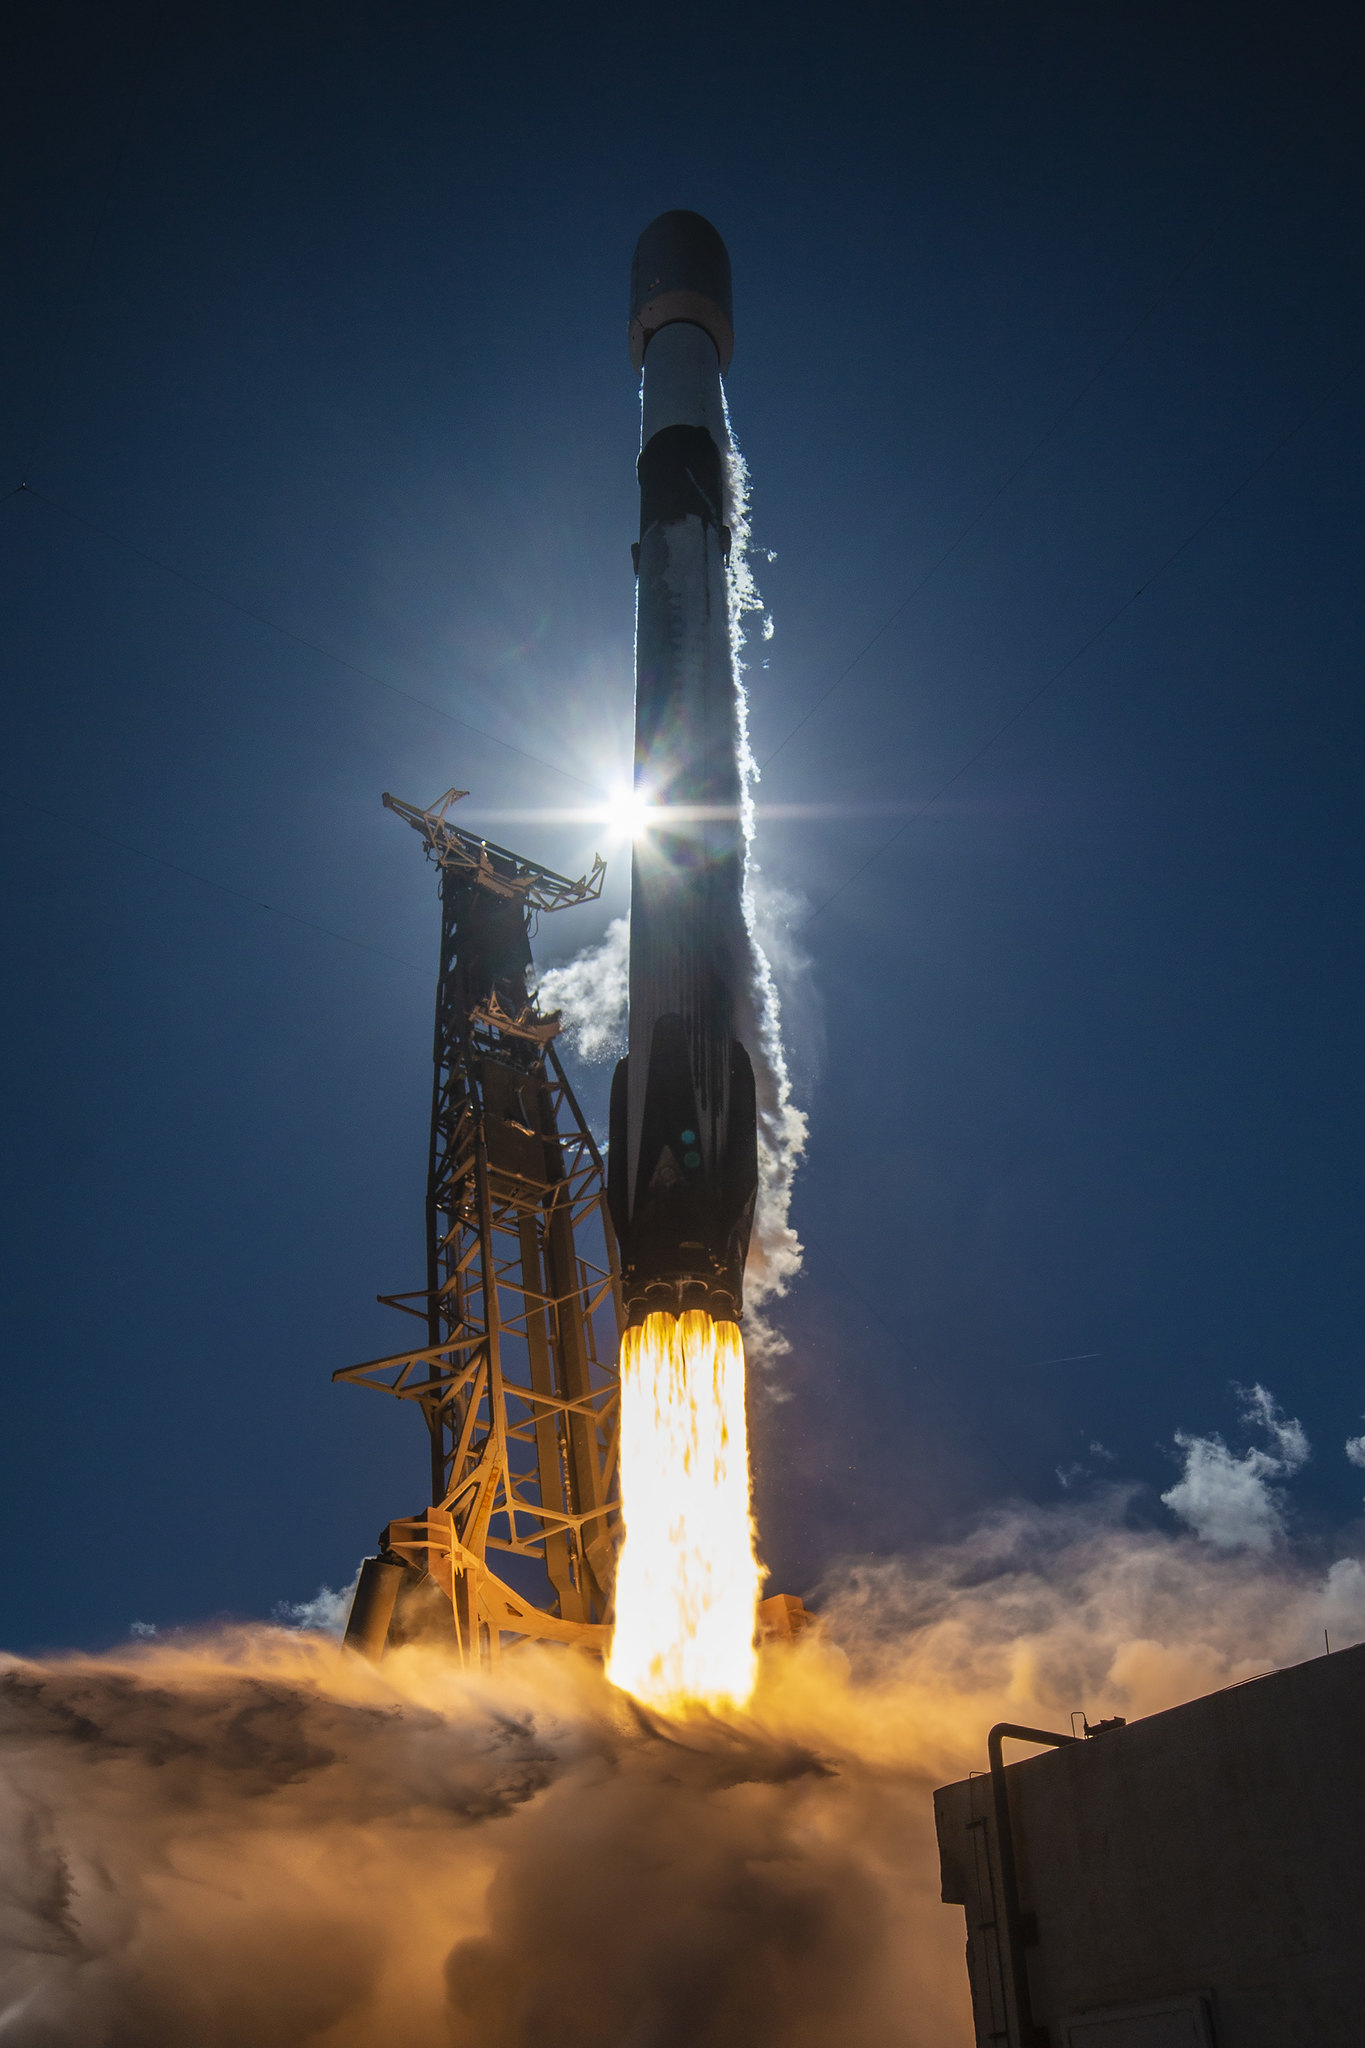
\includegraphics[height=7cm]{Figures/implementation/model/falcon_9.jpg}
    }\hfill
    \subfloat[New Shepard \cite{noauthor_blueorigin_nodate}\label{fig:new_shepard}]{
        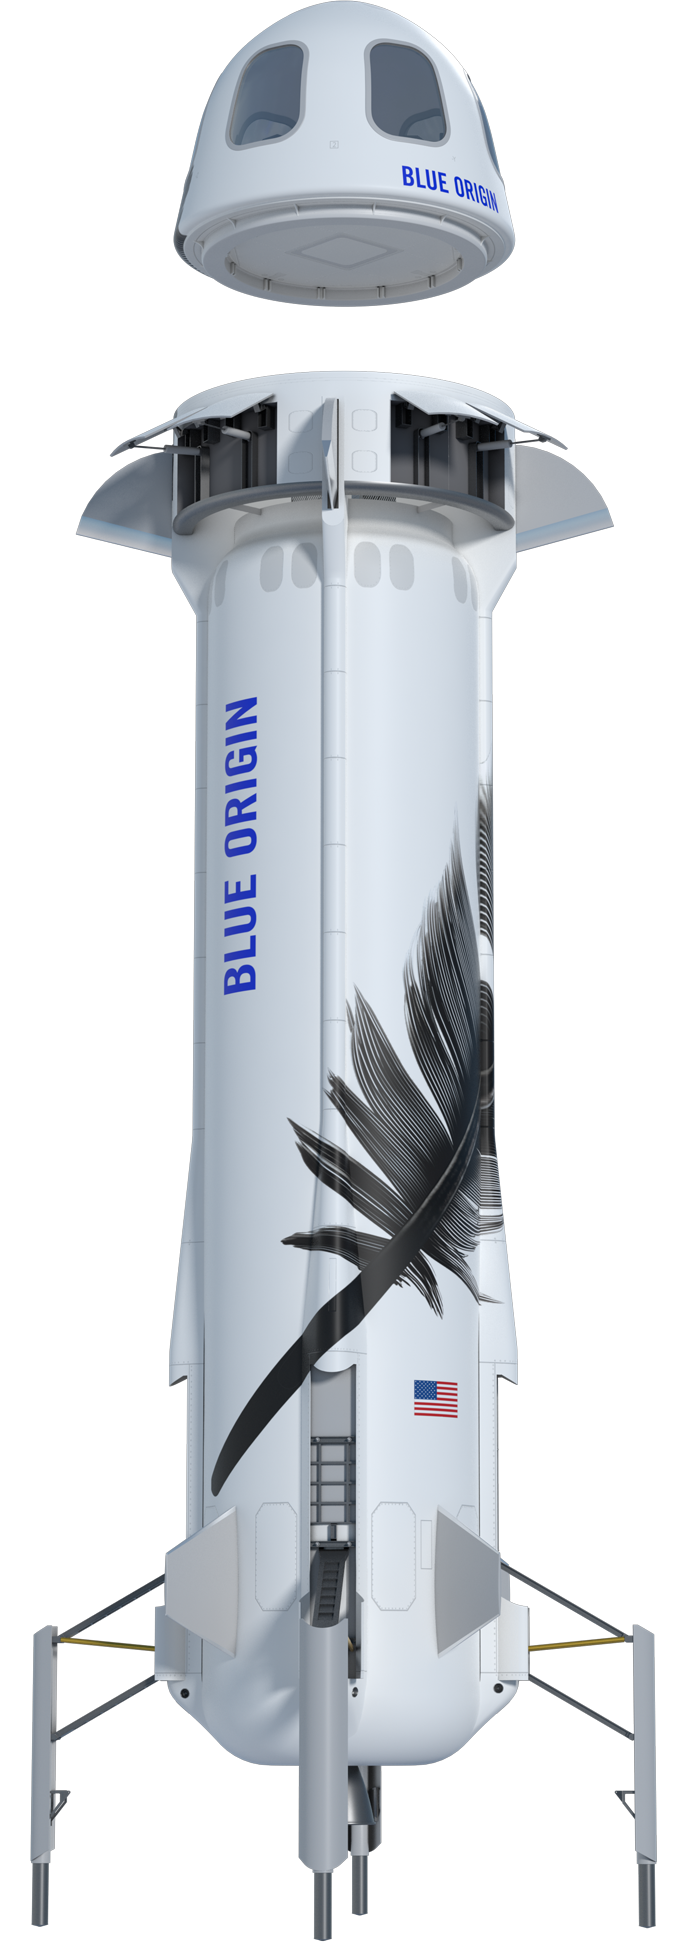
\includegraphics[height=7cm]{Figures/implementation/model/newshepard.png}
    }
    \caption{Spacecraft Vehicles operating nowadays}
    \label{fig:rocket_models}
\end{figure}

It is possible to understand that heavy launchers are mainly constructed under the same geometry: a cylinder. Also the previously referenced works \cite{maurer_project_nodate} and \cite{riegler_daedalus_2018} show a cylinder geometry for launchers Although it is a lighter and simpler vehicle which do not aim to achieve Earth's orbit. This means that the space industry still lies in cylinder format for its key component: the launcher.

So, before any other assumption, this thesis focus type of vehicle will be a simple cylinder with a rotor with a rotor on its top. Figure \ref{fig:vehicle_model}, presents the simplified vehicle considered. To easily define the geometry, it will be considered the geometry propreties shown in figure \ref{fig:vehicle_geometry}.


\begin{figure}[!htb]
    \centering
    \subfloat[Vehicle Model\label{fig:vehicle_model}]{
        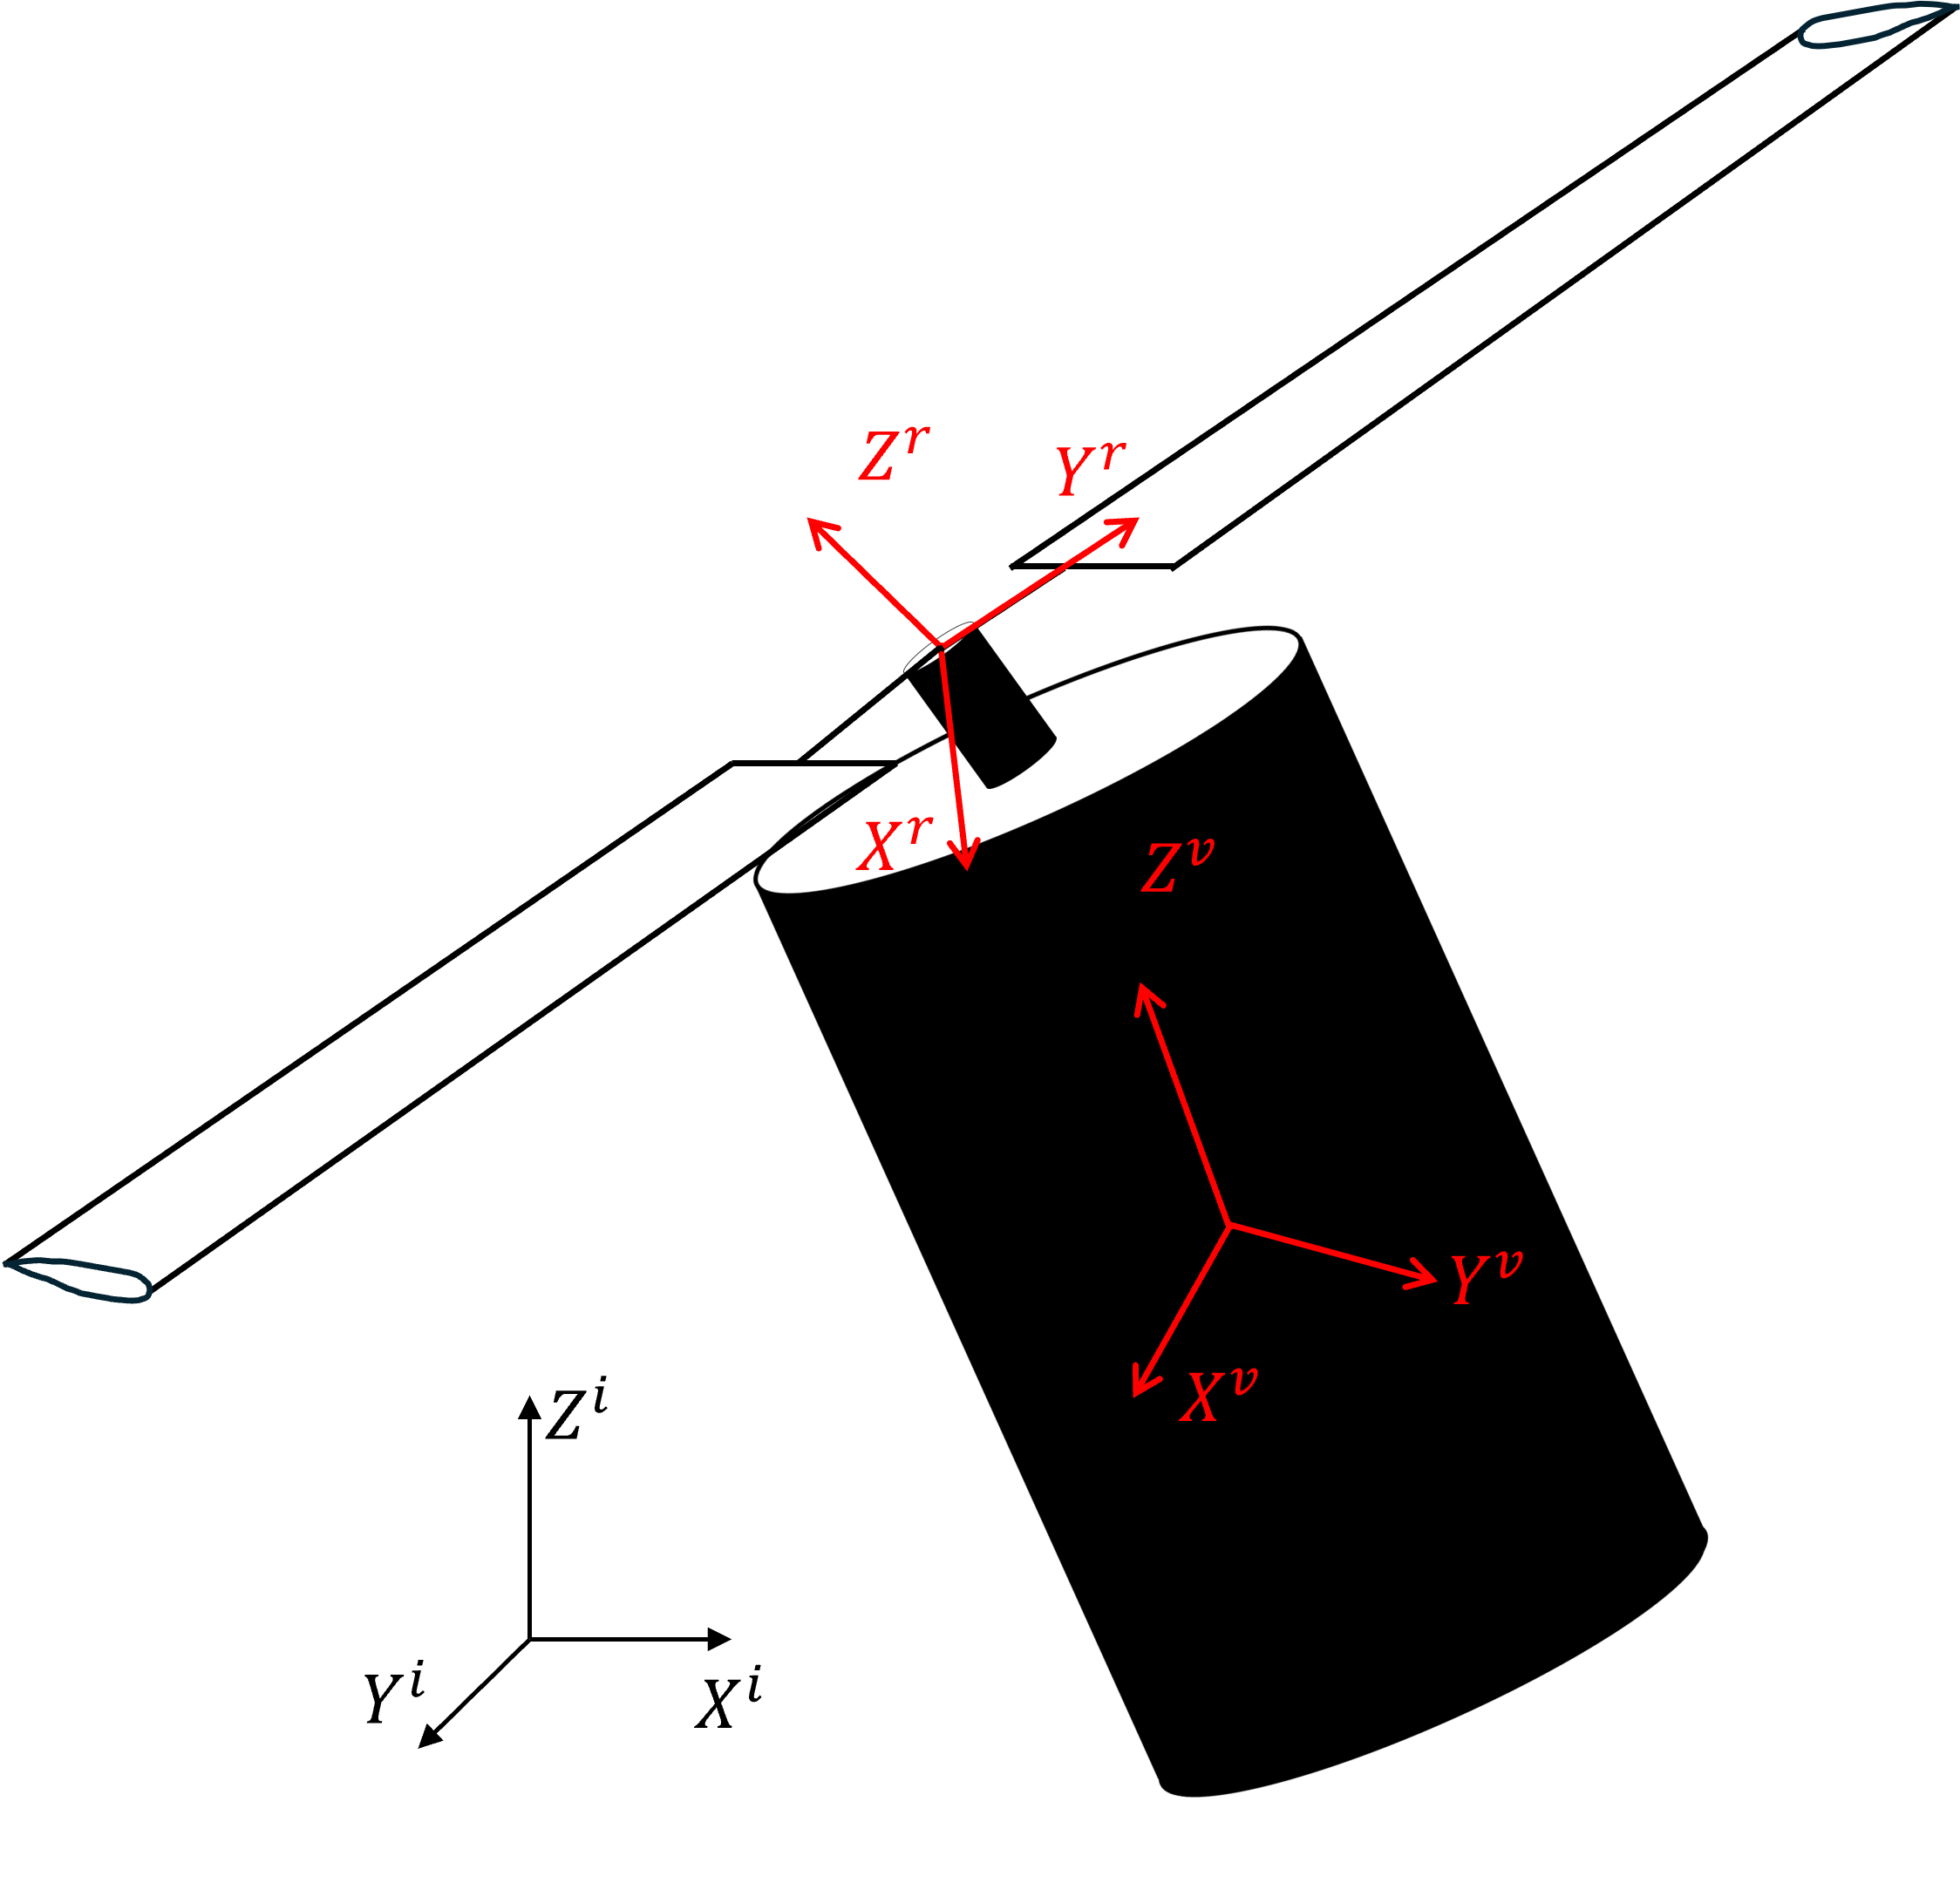
\includegraphics[height=6cm]{Figures/implementation/model/vehicle.png}
    }\hfill
    \subfloat[Vehicle Geometry proprieties\label{fig:vehicle_geometry}]{
        
\includegraphics[height=6cm]{Figures/implementation/model/geometry_proprieties.png}
    }
    \caption{Vehicle}
    \label{fig:vehicle}
\end{figure}


\subsection{Model simplications and assumptions}
\label{section:model_assumptions}

\textcolor{blue}{meter as simplicações aqui}

\begin{itemize}
    \item o corpo é rígido
    \item tem movimento de translação e rotação nos 3 eixos
    \item é deprezada a rotação da terra
    \item a terra é plana
\end{itemize}

\textcolor{blue}{falar sobre as metologias de alguns livros para mostrar o que usar em cada uma das partes do projeto}

\subsection{Reference Frames}
\label{section:referece_frames}

For the development of the mathematical model that follows and considering what was present in previous section \ref{section:model_assumptions} one must start by considering the reference frames which define the vehicle's dynamics. On figure \ref{fig:vehicle_model} the three principal references are presented: Earth referece frame, $O^i$, vehicle referece frame $O^v$ and rotor frame $O^r$.

The Earth frame, $O^i$, is a inertial frame positioned in any point of the Earth surface. It is also called \textit{Navigation Frame} once it rotates with Earth and it is very handy when planes to travel from one point to another \cite{soler_fundamentals_2014}. On other hand, the vehicle frame, $O^v$,  or body frame \cite{soler_fundamentals_2014} is a system axes centered in any point of the symmetry plane of the aircraft. In this case, the $O^v$ is position at the \gls{cg} of the vehive considering a two point mass system, one for the payload and one for the recovery system. The $O^v$ as its $z^v$-axis aligned from the \gls{cg} as shwon in figure \ref{fig:vehicle_model} for orietation reference. Finally, the rotor axes system, $O^r$ is centered in the rotor's hub and is aligned and has the same orietation as the $O^v$ reference frame.


\begin{figure}[!htb]
    \centering
        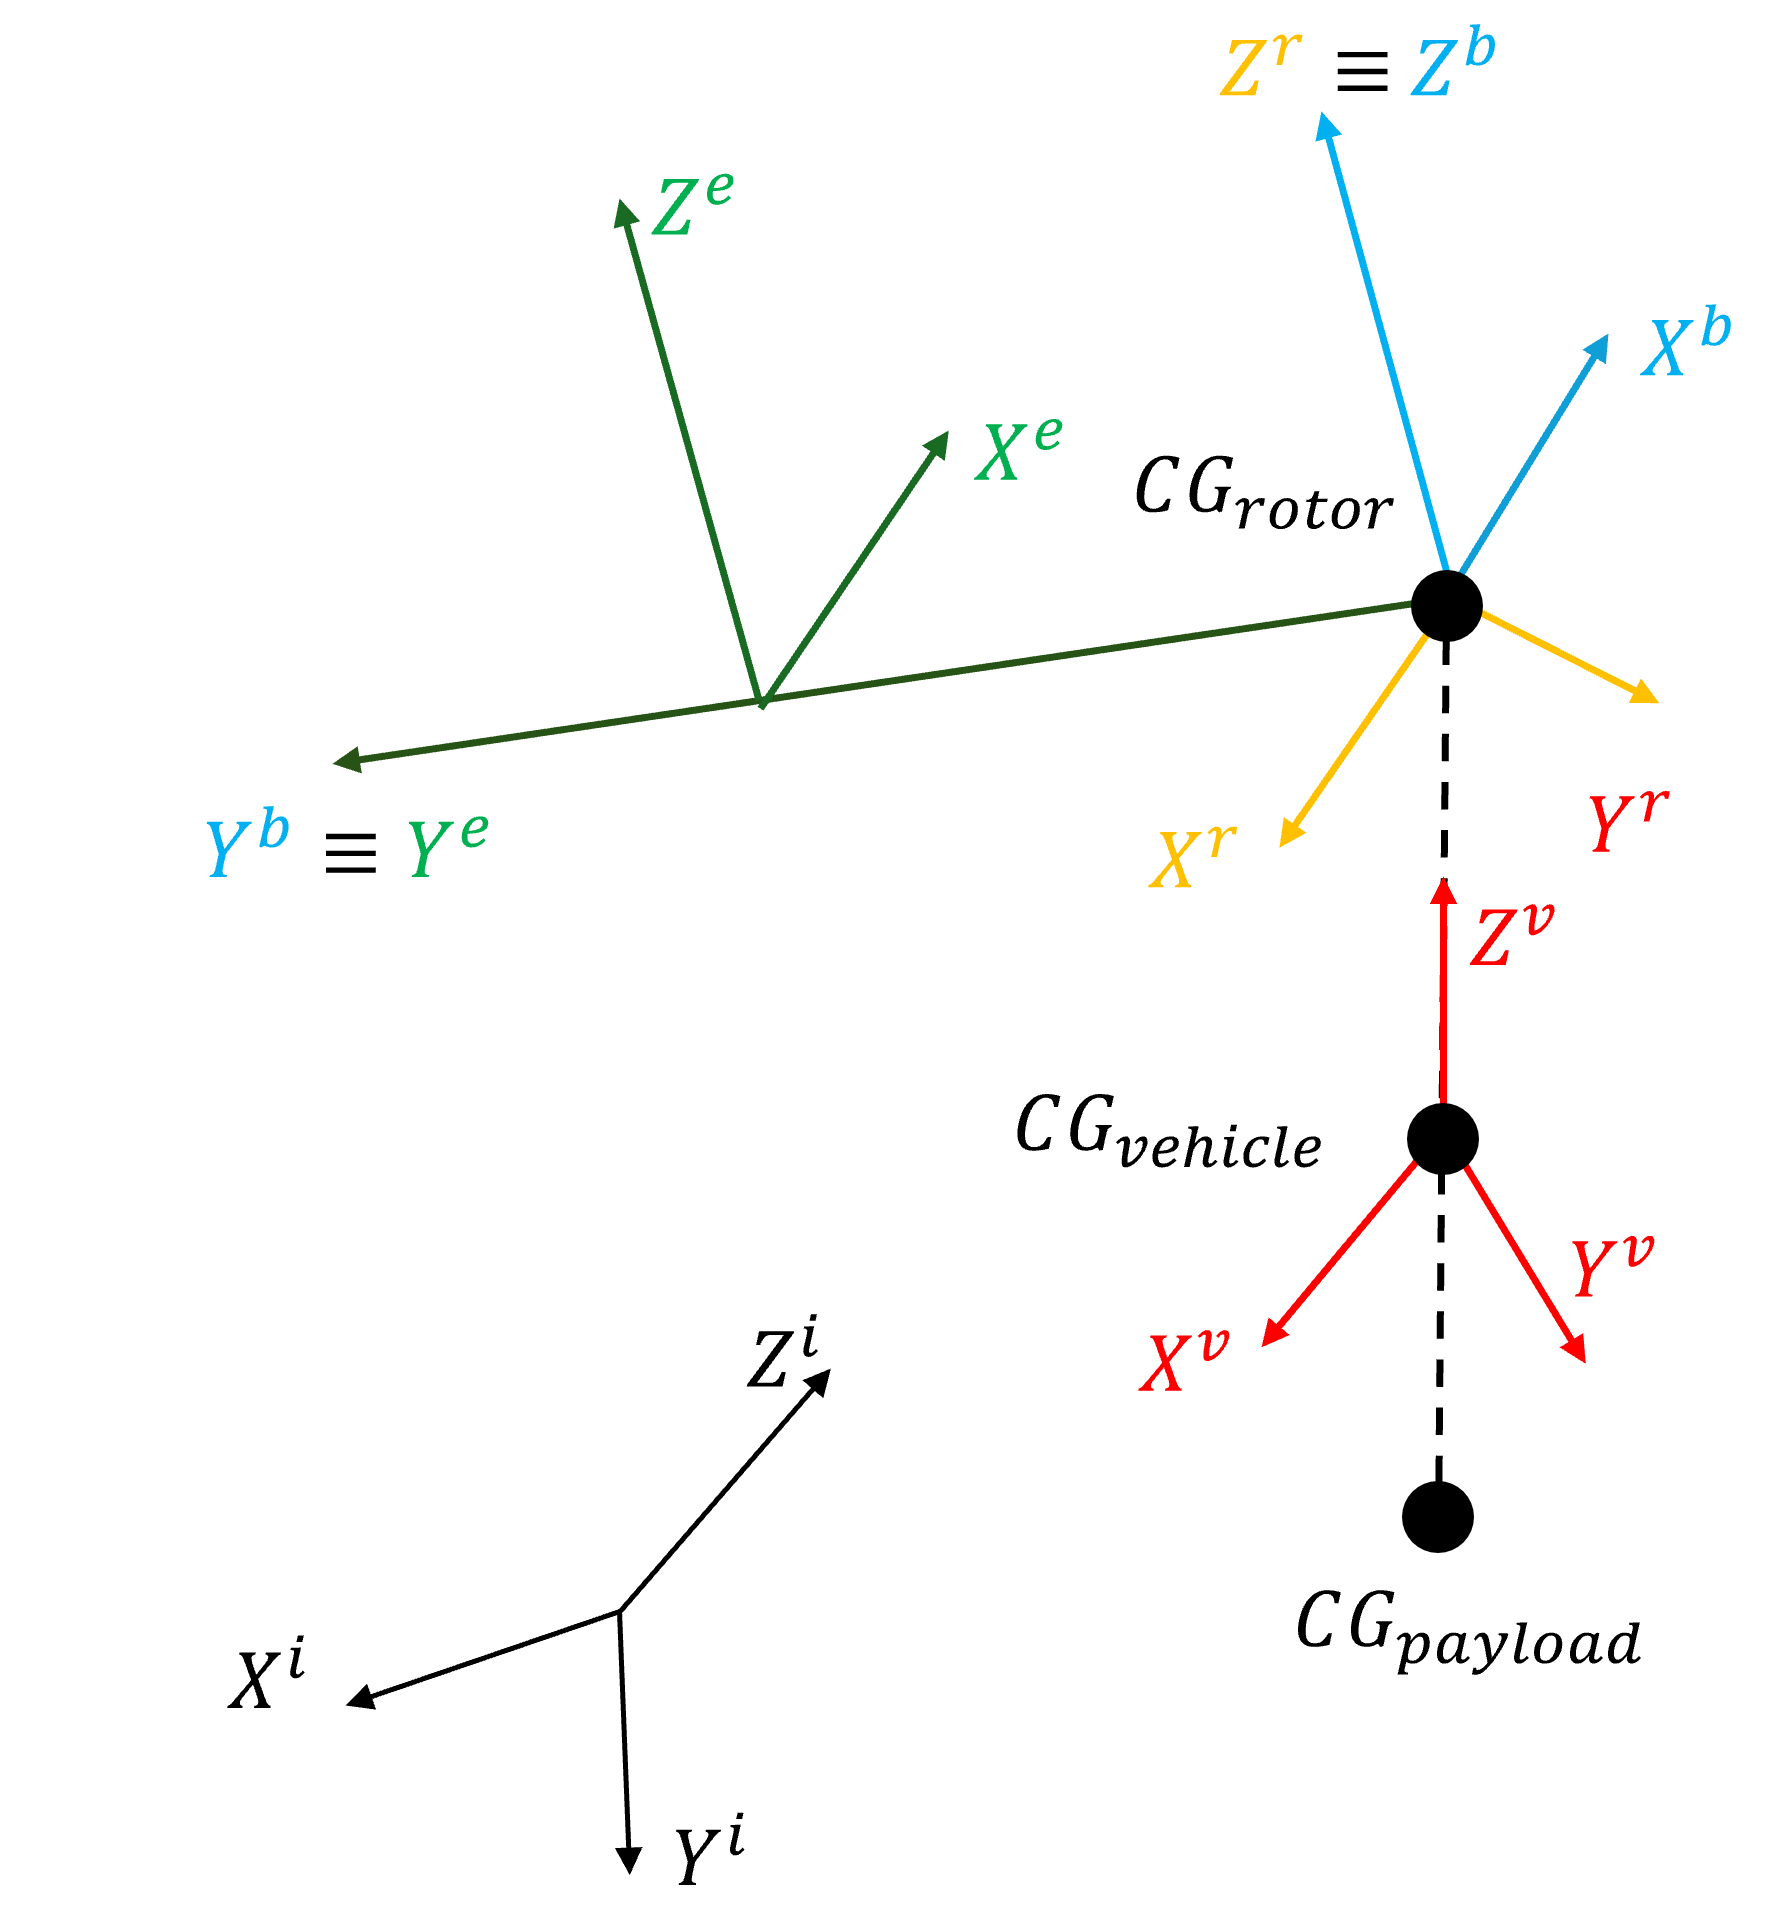
\includegraphics[width=8cm]{Figures/implementation/model/reference_frames_img.png}
        \caption{Model reference frames relation - as a simplication the figure was designed considering the that the viewer is aligned with $O^v \equiv O_r$ and the $O_i$ is rotated}
        \label{fig:reference_frames_img}
\end{figure}

The vehicle frame is positioned at the \gls{cg} of the vehicle total system and can be write in the $O^i$ as navigation coordinates,

\begin{equation}
    \mathbf{p}^i_{CG_{vehicle}} = \begin{bmatrix} x & y & z \end{bmatrix}^T \in \mathbb{R}^3.
\end{equation}

However, for moments calculations the position of the vehicle total system's \gls{cg} is a crucial point. As a simplification, previous mentioned in section \ref{section:model_assumptions}, the vehicle's \gls{cg} does not vary inside the vehicle. So, to determine the position of rotor's and payload's \gls{cg}, as presented in figure \ref{fig:reference_frames_img} relative to the overall system's \gls{cg} the vehicle´s geometry presented in figure \ref{fig:vehicle_geometry} are considered. The \gls{cg} of a system considering multiple mass point is given by equation \ref{eq:cg_position}

\begin{equation}
    \mathbf{R}_{CG} = \frac{\sum_{i} M_i \mathbf{R}_i}{\sum_{i} M_i}
    \label{eq:cg_position}
\end{equation}

and fixing a $O'$ auxiliary reference frame at the vehicle’s bottom with its $z$-axis aligned with $O^v$ $z$-axis and setting the payload's and rotor's mass to be at $z$-axis, the \gls{cg} position of the vehicle, \( z^{O'}_{CG_{\text{vehicle}}} \), is given by

\begin{equation}
    z^{O'}_{CG_{\text{vehicle}}} = \frac{\frac{1}{2} M_{\text{payload}} H_{\text{payload}} + \left(H_{\text{hub}} + H_{\text{payload}}\right) M_{\text{rotor}}}{M_{\text{payload}} + M_{\text{rotor}}}
\end{equation}

Then, to define the payload's and rotor's \gls{cg} position relative to \( O_v \):

\begin{equation}
    z^{v}_{CG_{\text{payload}}} = z^{O'}_{CG_{\text{vehicle}}} - \frac{1}{2} H_{\text{payload}}
\end{equation}

and

\begin{equation}
    z^{v}_{CG_{\text{rotor}}} = H_{\text{payload}} + H_{\text{hub}} - z^{O'}_{CG_{\text{vehicle}}}.
\end{equation}

Finally, the in vector form, the position is given by

\begin{equation}
    \mathbf{r}_{O_{\text{payload}}}^v =  \begin{bmatrix} 0 & 0 & -z^{v}_{CG_{\text{payload}}} \end{bmatrix} \quad \text{and} \quad \mathbf{r}_{O_{\text{rotor}}}^v =  \begin{bmatrix} 0 & 0 & z^{v}_{CG_{\text{rotor}}} \end{bmatrix}.
\end{equation}


In terms of $O^v$ and $O^r$ orietation, the approach that is used is the common Tailt-Bryan
Convention \cite{soler_fundamentals_2014} as it is used in many flight dynamics textbooks as Cook \cite{cook_flight_2007} and Vepa \cite{vepa_flight_2023}. The Tailt-Bryan Convention defines a sequence of rotation being the first angle of rotation around the $z$-axis, the second around the  $y$-axis, and the third around the  $x$-axis. Meaning the $z$-axis the yaw angle,  $y$-axis the pitch angle , and $x$-axis the roll angle This angles are known as Euler angles and will be presented from now on as

\begin{equation}
    \boldsymbol{\eta} \equiv \left(\eta_1, \eta_2, \eta_3 \right)
    \label{eq:euler_angles_vehicle}
\end{equation}

for the vehicles reference frame, $O^r$, orientation relatively to the inertial frame, $O^i$, and

\begin{equation}
    \boldsymbol{\zeta} \equiv \left(\zeta_1, \zeta_2, \zeta_3 \right)
    \label{eq:euler_angles_rotor}
\end{equation}

for the vehicles reference frame, $O^i$, orientation relatively to the vehicle frame, $O^v$. The $O^v$ rotates relatively to $O^i$ and the three component vector where defined in equation \ref{eq:euler_angles_vehicle}. On the other hand, $O^r$ rotates relatively to $O^v$ and the vecor is defined in \ref{eq:euler_angles_rotor}, then to study the dynamics of the problem, there is a need for defining the rotation matrices.

Considering any inertial reference frame $O(X,Y,Z)$ and a rotated reference frame $O'(X',Y',Z')$, the Euler angles, $\Xi$ that the define the rotation of $O'$ related to $O$ is presented in figure \ref{fig:rotation_frames_img}

\begin{figure}[!htb]
    \centering
        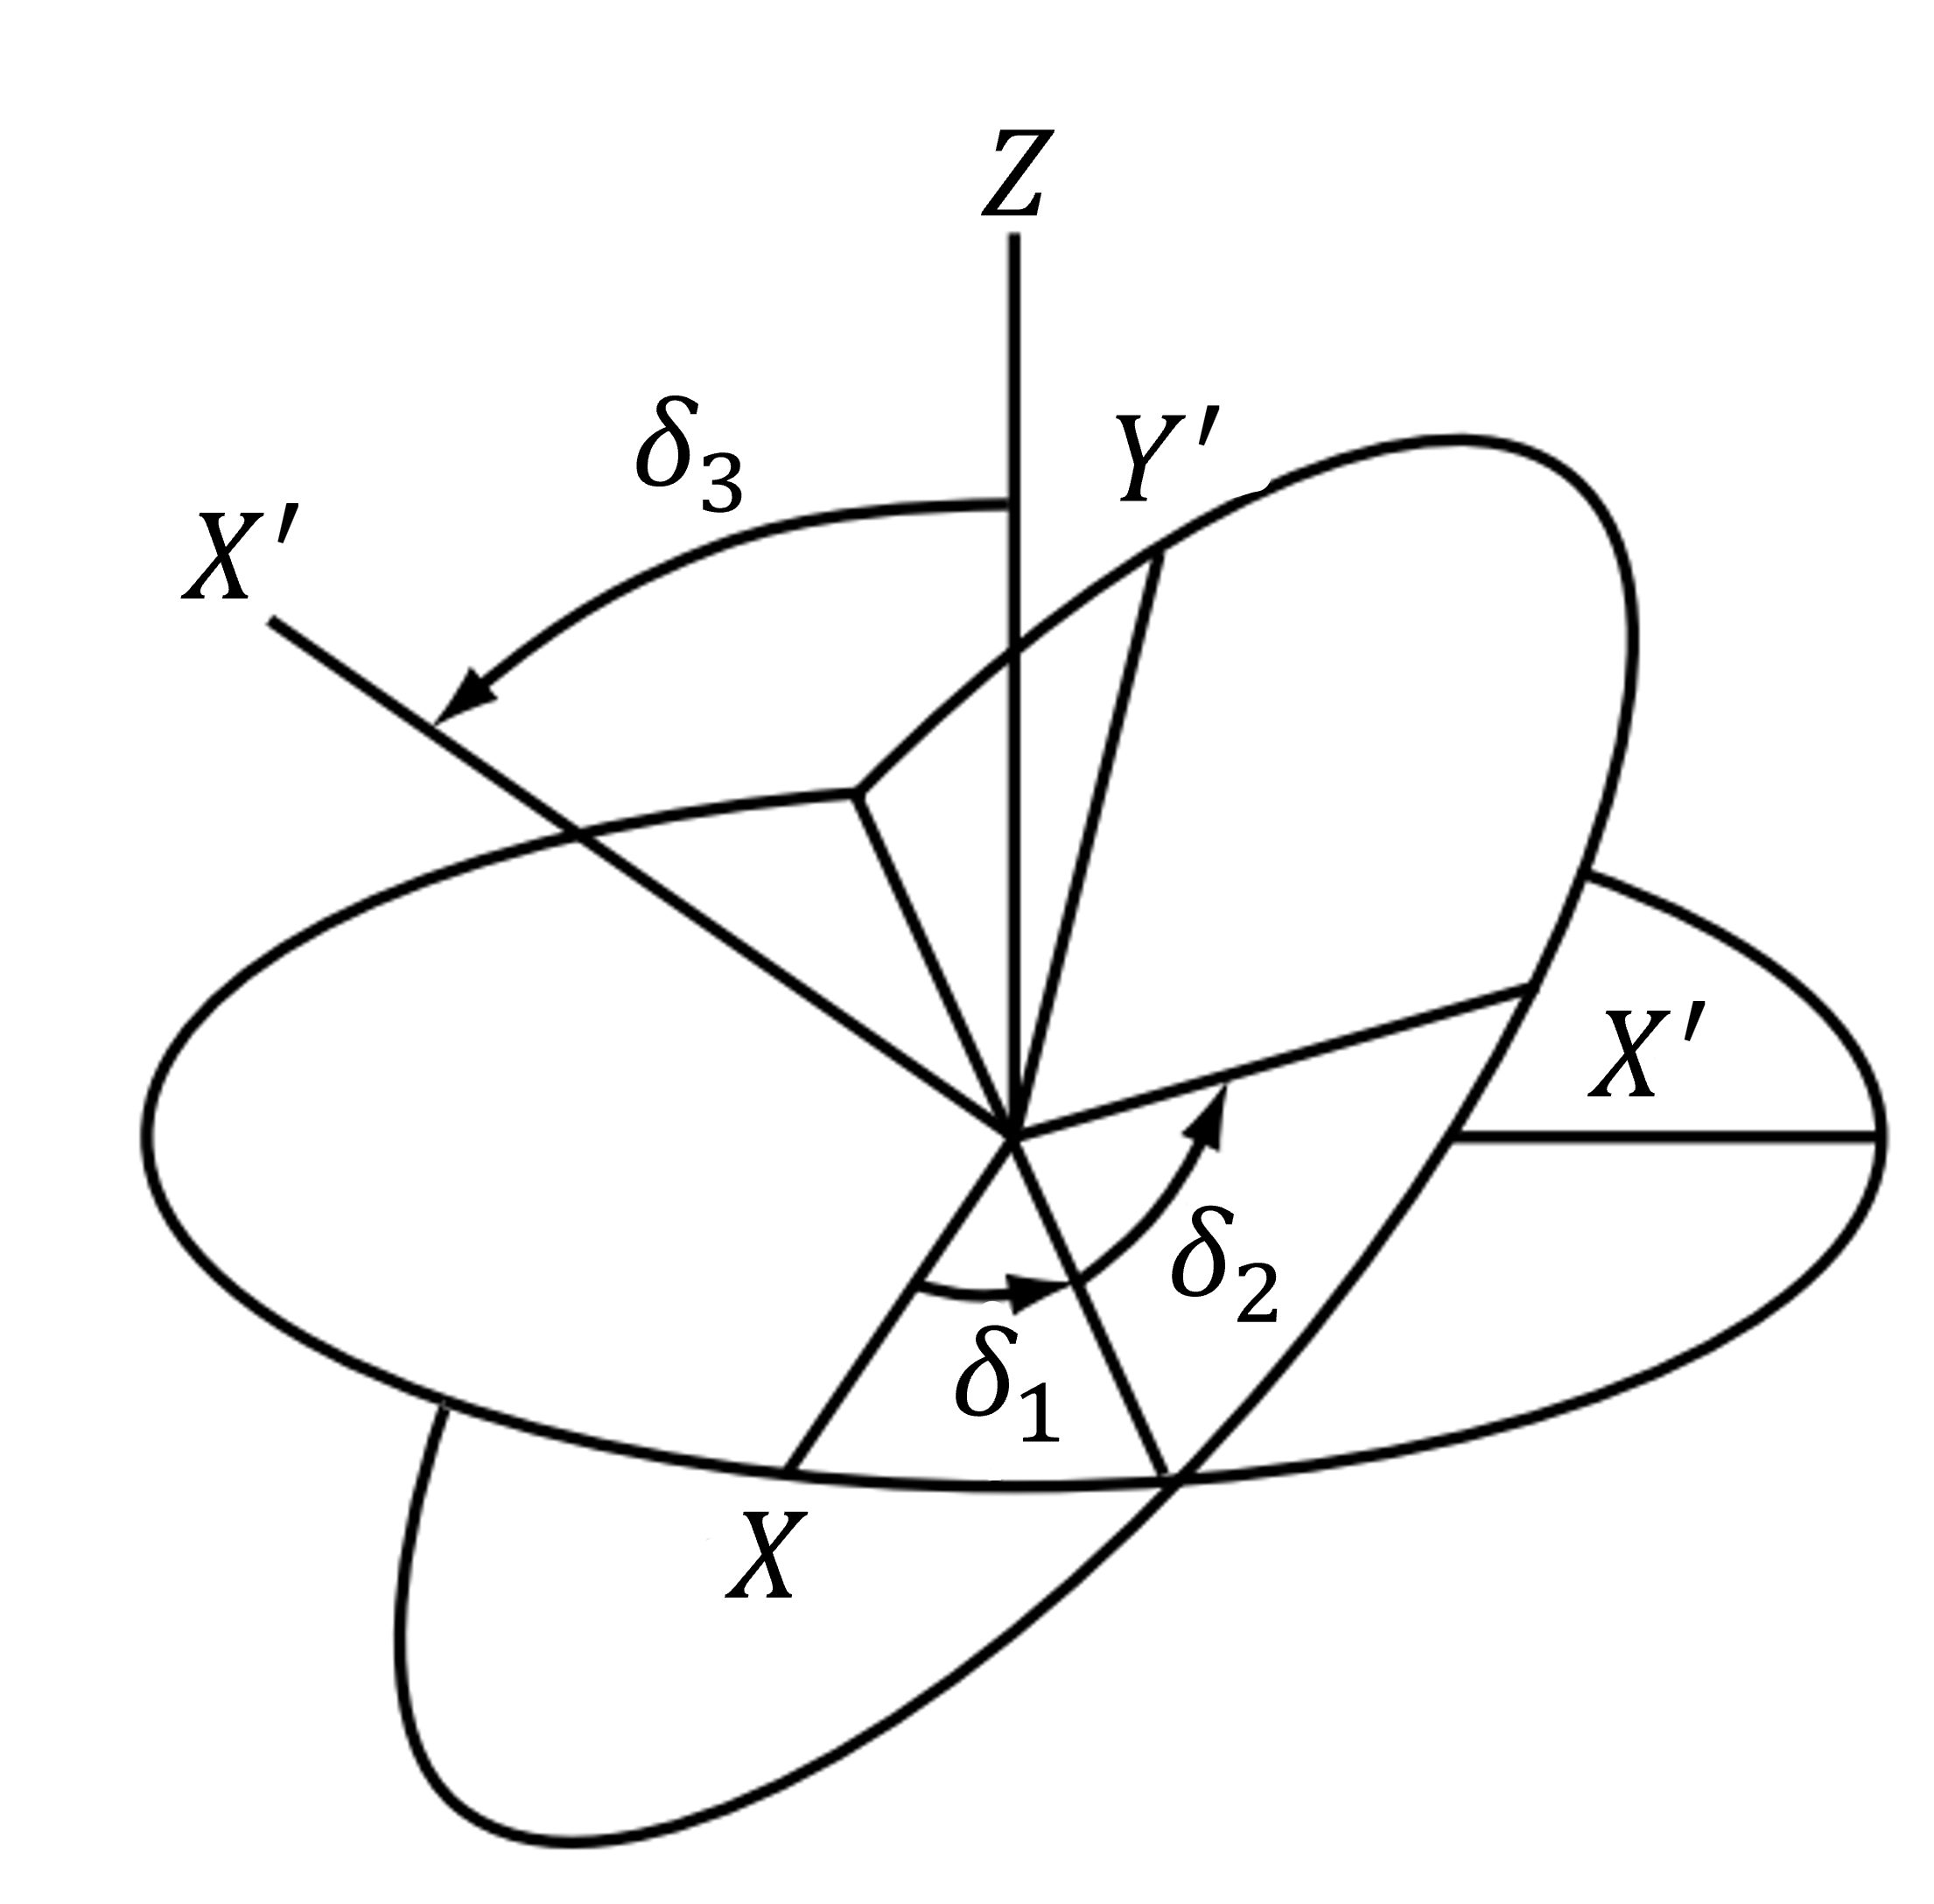
\includegraphics[width=6cm]{Figures/implementation/model/rotation_frames.png}
        \caption{Reference frame rotation Euler angles, adapted from \cite{schwab_how_2006}}
        \label{fig:rotation_frames_img}
\end{figure}

The following expressions, presented in equations \ref{eq:rotatio_zz}, \ref{eq:rotatio_yy} and \ref{eq:rotatio_xx}, define the rotation matrices of a rotation over the each of the reference axis $\hat{Z}$, $\hat{Y}$ and $\hat{X}-$axis. Also each equation present de derivetive of the rotation matrix which will be needed later on this mathematical model.

\begin{equation}
    {R o t({\hat{Z}},\eta_1)}={\left[\begin{array}{l l l}{1}&{0}&{0}\\ {0}&{c_{\eta_1}}&{-s_{\eta_1}}\\ {0}&{s_{\eta_1}}&{c_{\eta_1}}\end{array}\right]} \quad \text{and} \quad \frac{\mathrm{d}Rot(\hat{Z}, \eta_3)}{\mathrm{d}t}  = \begin{bmatrix} 0 & 0 & 0 \\ 0 & -s_{\eta_1} \dot{\eta_1} & -c_{\eta_1} \dot{\eta_1} \\ 0 & c_{\eta_1} \dot{\eta_1} & -s_{\eta_1} \dot{\eta_1} \end{bmatrix}
    \label{eq:rotatio_zz}
\end{equation}

\begin{equation}
    Rot(\hat{Y},\eta_2)=\left[\begin{array}{c c c}{{c_{\eta_2}}}&{{0}}&{{s_{\eta_2}}}\\ {{0}}&{{1}}&{{0}}\\ {{-s_{\eta_2}}}&{{0}}&{{c_{\eta_2}}}\end{array}\right] \quad \text{and} \quad \frac{\mathrm{d}Rot(\hat{Y}, \eta_2)}{\mathrm{d}t} = \left[\begin{array}{c c c}-s_{\eta_2} \dot{\eta_2} & 0 & c_{\eta_2} \dot{\eta_2} \\ 0 & 0 & 0 \\ -c_{\eta_2} \dot{\eta_2} & 0 & -s_{\eta_2} \dot{\eta_2} \end{array}\right]
    \label{eq:rotatio_yy}
\end{equation}

\begin{equation}
    Rot({\hat{ X}},{\delta_3})={\left[\begin{array}{l l l}{{{c}_{\delta_3}}}&{{-{s}_{\delta_3}}}&{{0}}\\ {{{s}_{\delta_3}}}&{{{c}_{\delta_3}}}&{{0}}\\ {{0}}&{{0}}&{{1}}\end{array}\right]} \quad \text{and} \quad \frac{\mathrm{d}Rot(\hat{X}, \delta_3)}{\mathrm{d}t} = \left[\begin{array}{c c c}
        -s_{\eta_3} \dot{\eta_3} & -c_{\eta_3} \dot{\eta_3} & 0 \\
        c_{\eta_3} \dot{\eta_3} & -s_{\eta_3} \dot{\eta_3} & 0 \\
        0 & 0 & 0
        \end{array}\right]
        \label{eq:rotatio_xx} 
\end{equation}

For the rotation matrices, it is used a simplified nomenclature where $c_{\eta_{*}}$ and $s_{\eta_{*}}$ are cosine and sine functions of the angle $\eta_{*}$. The total rotation matrix, considering the Tailt-Bryan Convention is

\begin{equation}
    Rot(\boldsymbol{\Xi})= Rot(\hat{Z},\eta_1) \cdot Rot(\hat{Y},\eta_2) \cdot Rot(\hat{X},\eta_3)
    \label{eq:total_rotation_matrix}
\end{equation}

while the derivative of the total rotation matrix is given by equation

\begin{equation}
    \frac{\mathrm{d}Rot(\boldsymbol{\Xi})}{\mathrm{d}t}= \frac{\mathrm{d}}{\mathrm{d}t} \left[Rot(\hat{Z},\eta_1) \cdot Rot(\hat{Y},\eta_2) \cdot Rot(\hat{X},\eta_3)\right].
    \label{eq:derivative_total_rotation_matrix}
\end{equation}

Proceeding with some mathematical development applying the chain rule, equation \ref{eq:derivative_total_rotation_matrix}  ca be simplified and the derivative of the total rotation matrix is


\begin{equation}
    \begin{aligned}
        \frac{\mathrm{d} \, Rot(\boldsymbol{\Xi})}{\mathrm{d}t} &= 
        \frac{\mathrm{d} Rot(\hat{Z}, \eta_1)}{\mathrm{d}t} \cdot Rot(\hat{Y}, \eta_2) \cdot Rot(\hat{X}, \eta_3) \\
        &\quad + Rot(\hat{Z}, \eta_1) \cdot \frac{\mathrm{d} Rot(\hat{Y}, \eta_2)}{\mathrm{d}t} \cdot Rot(\hat{X}, \eta_3) \\
        &\quad + Rot(\hat{Z}, \eta_1) \cdot Rot(\hat{Y}, \eta_2) \cdot \frac{\mathrm{d} Rot(\hat{X}, \eta_3)}{\mathrm{d}t}
    \end{aligned}.
    \label{eq:exp_derivative_total_rotation_matrix}
\end{equation}


Besides presenting, the previous reference frames and the relation between them, figure \ref{fig:reference_frames_img} shows another two complementary reference frames that will be further useful in \ref{sec:BET} section where a deeper insight is made about \gls{bet}. As a first introduction, the first reference frame is the blade frame, $O^b$, over which the blade's element force will be integrated to compute the total blade force, and the element reference frame, $O^e$, over which the elementary force will be calculated. A more detailed overview is done in section \ref{sec:BET} in which \gls{bet} is presented.


\subsection{System's Degrees of Freedom}

Before advance into a more advanced insight of the vehicle's laws of motion, it is importante to explain how the deegrees of freedom are. Firtsly, the translational movement in a inertial frame, due to the freefall, happens in an tri-dimensional space, once the vehicle can glide. This defines the 3-\gls{dof}. Also, the payload can rotate freely about its \gls{cg}, what means that another 3-\gls{dof} are defined once the rotation can occur along each axis. Finally, the rotor can also rotate around its hub joint cooupled at the payload's top which means three degree of freedom are needed to define the rotor's dynamic. In vector form, the state that describes the vehicle instantaneous state is 

\begin{equation}
    \aleph = \begin{bmatrix}
        x & y & z & \eta_1 & \eta_2 & \eta_3 & \zeta_1 & \zeta_2 & \zeta_3
    \end{bmatrix}^T
\end{equation}

where $x$, $y$, and $z$ are the coordinates of the vehicle's center of gravity (CG) in the inertial frame, components of $\mathbf{p}_{CG_{vehicle}}$. The vehicle's orientation is defined by Euler angles $\eta_1$, $\eta_2$, $\eta_3$ components of $\boldsymbol{\eta}$, and $\eta_1$, $\eta_2$, $\eta_3$ components of $\boldsymbol{\zeta}$ are the rotor orietation in the vehicle's frame.


%%%%%%%%%%%%%%%%%%%%%%%%%%%%%%%%%%%%%%%%%%%%%%%%%%%%%%%%%%%%%%%%%%%%%%%%
\section{7-DOF Vehicle Dynamics}
\label{section:vehicle_dynamics}

After identify the refrence frames and the vehicle's key states, it is time to introduce the strategy which easily ables to mathematically express the recovery system motion. The analysis will be separated in two parts. The first part is about vehicle the vehicle 6-\gls{dof} and its present in section \ref{section:Vehicle_Motion} and the secont part deals with the last \gls{dof}, in section \ref{section:rotor_Motion}, the rotation of the rotor. This strategy simplifies the mathematical development by decoupling the complexity of moment transfer from the rotor to the payload.


\subsection{Vehicle Motion}
\label{section:Vehicle_Motion}


The dynamics of vehicles with six degrees of freedom (6-DOF) are governed by Newton's Second Law, which relates the sum of forces (moments) acting on a body to its linear (or angular) acceleration. In this framework, define by equation \cite{cook_flight_2007}, both translational and rotational motions are considered within a three-dimensional space, making it essential for analyzing vehicles that move freely in all three spatial directions $(x, y, z)$ and rotate around their principal axes (roll, pitch, and yaw). 

For translational movement in the inertial frame, the resulting force $\mathbf{F}^i$ is given by the product of the vehicle's mass $M$ and its acceleration, $\mathbf{A}^i$, as shown in equation \ref{eq:second_law_newton}. 

\begin{equation}
    \mathbf{F}^i  = M \cdot \mathbf{A}^i
    \label{eq:second_law_newton}
\end{equation}

in the inertial frame, being the resulting force composed by the components, in the same frame, gravity, $\mathbf{F}_G^i$, the rotor force $\mathbf{F}_R^i$ and vehicle aerodynamic drag, $\mathbf{F}_{Drag}^i$,

\begin{equation}
    \mathbf{F}^i = \mathbf{F}_G^i + \mathbf{F}_R^i + \mathbf{F}_{Drag}^i.
\end{equation}

and the vehicle's mass composed by the sum of the payload's mass, $M_{payload}$, and rotor's mass , $M_{rotor}$,

\begin{equation}
    M = M_{payload} + M_{rotor}
\end{equation}


The translational velocity, $\mathbf{V}^i$,  is 

\begin{equation}
    \frac{\mathrm{d}\mathbf{V}^i}{\mathrm{d}t}\equiv  \dot{\mathbf{V}}^i = \mathbf{A}^i = \frac{1}{M} \cdot \mathbf{F}^i
\end{equation}

The reference frame is at the center of the vehicle body \gls{cg}, so there is no relative position with respect to the vehicle frame, so the position of the vechile in inertial frame, $\mathbf{P}^i$, is

\begin{equation}
    \frac{\mathrm{d}\mathbf{P}^i}{\mathrm{d}t} \equiv \dot{\mathbf{P}}^i = \mathbf{V}^i
    \label{eq:navigation_coordinates}
\end{equation}

For the rotational movement of the vehicle arounf its \gls{cg}, the second Newton's law in the vehicle frame is given by

\begin{equation}
    \mathbf{M}^i =  \frac{\mathrm{d}}{\mathrm{d}t}\mathbf{H}^i \equiv \dot{\mathbf{H}}^i
    \label{eq:total_moments_expr}
\end{equation}

where $\left[\mathbf{I}\right]^i$ is the moments vector  along each principal axis in inertial frame and $\dot{\mathbf{H}}$ is the rate of change of the angular momentum 

\begin{equation}
    \mathbf{H}^i = \left[\mathbf{I}\right]^i \boldsymbol{\omega}_{vehicle}^i
    \label{eq:angular_momentum}
\end{equation}

where $\mathbf{I}^v$ is the second moments of inertia and $\boldsymbol{\omega}_{vehicle}$ is the angular velocity in in $O^i$. Subtituting \ref{eq:angular_momentum} into \ref{eq:total_moments_expr} the equation is


\begin{equation}
    \mathbf{M}^i =  \dot{\left[\mathbf{I}\right]}^i \boldsymbol{\omega}_{vehicle}^i + \left[\mathbf{I}\right]^i\dot{\boldsymbol{\omega}}_{vehicle}^i
    \label{eq:total_moment_derivatives}
\end{equation}

Some considerations shall be made about equation \ref{eq:total_moment_derivatives}. Once the theres a degree of freedom due to the rotor rotation, the second moments of inertia matrix, $\left[\mathbf{I}\right]^i$, is not contant over time. To simplify this approach, the angular momentum $\mathbf{H}^i$, can be computed in in the vehicle frame, $O^v$, for equation \ref{eq:total_moments_expr}, as

\begin{eqnarray}
    \mathbf{M}^i =  \dot{\mathbf{H}}^v + \boldsymbol{\Omega}_{REF} \times \mathbf{H}^v
\end{eqnarray}

and then

\begin{equation}
    \mathbf{M}^i = \frac{\mathrm{d}}{\mathrm{d}t} \left(\left[\mathbf{I}\right]^v \boldsymbol{\omega}_{\text{vehicle}}^v\right) + \boldsymbol{\Omega}_{REF} \times \left(\left[\mathbf{I}\right]^v \boldsymbol{\omega}_{\text{vehicle}}^v\right)
\end{equation}

Once $\dot{\left[\mathbf{I}\right]}^v = 0$, then

\begin{equation}
    \mathbf{M}^i =\left[\mathbf{I}\right]^v \dot{\boldsymbol{\omega}}_{vehicle}^v + \boldsymbol{\Omega}_{REF} \times \left(\left[\mathbf{I}\right]^v \boldsymbol{\omega}_{\text{vehicle}}^v\right)
\end{equation}


\textcolor{red}{fiquei aquiiiiiiiii na equação de cima}

with a constant $\mathbf{I}^r$ once the rotor is always aligned withe $O^r$ and the cilinder does not made any change in $\mathbf{I}^r$. The total moment, $\mathbf{M}^r$, is 

\begin{equation}
    \mathbf{M}^r = \mathbf{M}_G^r + \mathbf{M}_R^r + \mathbf{M}_{Drag}^r.
\end{equation}

Where $\mathbf{M}_G^r$ is the moment caused from gravity in each point mass force, $\mathbf{M}_R^r$ from the rotor force and $\mathbf{M}_{Drag}^r$ from the vehicle aerodynamic drag. The vehicle's angular velocity, $\boldsymbol{\omega}^r_{vehicle}$, in $O^r$ is

\begin{equation}
    \frac{\mathrm{d}\boldsymbol{\omega}^r_{vehicle}}{\mathrm{d}t} \equiv \boldsymbol{\dot{\omega}}^r_{vehicle} = \boldsymbol{\chi}^r_{vehicle} = (\mathbf{I}^r)^{-1} \mathbf{M}^r.
    \label{eq:angular_acceleration_inRotor}
\end{equation}

However, the interest is the angular acceleration in the $O^v$. So, to obtain the anguar acceleration in $O^v$

\begin{equation}
    \boldsymbol{\chi}^r_{vehicle} = \boldsymbol{R}^*_{v \rightarrow r} \boldsymbol{\chi}^v_{vehicle} \implies \boldsymbol{\chi}^v_{vehicle} = \left(\boldsymbol{R}^*_{v \rightarrow r}\right)^{-1} \boldsymbol{\chi}^r_{vehicle}
    \label{eq:angular_acceleration_inVehicle}
\end{equation}

Using equation \ref{eq:angular_acceleration_inVehicle} into equation \ref{eq:angular_acceleration_inRotor}, the vehicles angular acceleration around its \gls{cg} is

\begin{equation}
    \boldsymbol{\dot{\omega}}^v_{vehicle} = \left(\boldsymbol{R}^*_{v \rightarrow r}\right)^{-1} (\mathbf{I}^r)^{-1} \mathbf{M}^r.
\end{equation}


and the angular position which shall be considered as a rotation of $O^v$ in $O^i$, so


\begin{equation}
    \frac{\mathrm{d}\boldsymbol{\Xi}^i_{vehicle}}{\mathrm{d}t} \equiv \dot{\boldsymbol{\Xi}}^i_{vehicle} = \boldsymbol{\omega}^i_{vehicle}
\end{equation}

The angular velocity was previously presented in \ref{eq:angular_acceleration_inVehicle}, but needs to be written in $O^i$ to compute vehicle orientation considerting euler angles the Euler angles. Then,

\begin{equation}
    \boldsymbol{\omega}^v_{vehicle} = \boldsymbol{R}^*_{i \rightarrow v} \boldsymbol{\omega}^i_{vehicle} \implies \boldsymbol{\omega}^i_{vehicle} = \left(\boldsymbol{R}^*_{i \rightarrow v}\right)^{-1} \boldsymbol{\omega}^v_{vehicle} 
\end{equation}

and finally the vehicle's orientation equation is

\begin{equation}
    \dot{\boldsymbol{\Xi}}^i_{vehicle} = \left(\boldsymbol{R}^*_{i \rightarrow v}\right)^{-1} \boldsymbol{\omega}^v_{vehicle} 
\end{equation}

\subsection{Rotor Motion}
\label{section:rotor_Motion}

To desbribe the rotor motion, a very simple simplication can be made once only one degree of freedom is defined. The rotation is about the vertical axis either for $O^v$ and for $O^r$. Also, the only force, needed to be considered in this dynamic, is the in-plane propulsive force generated during the phenomena of autorotation.

The rotor montion is defined by a single equation and can be deduced as for the vehicle´s rotation throw its \gls{cg}. The velocity in $O^v$ of the rotor is 


\begin{equation}
    \frac{\mathrm{d}\omega^v_{rotor}}{\mathrm{d}t} \equiv \dot{\omega}^v_{rotor} \equiv \dot{\omega}^r_{rotor} = \frac{1}{I^r_{x_{rotor}}} M^r_{rotor}
\end{equation}

The position can be simply computed as

\begin{equation}
    \frac{\mathrm{d}\Psi^v_{rotor}}{\mathrm{d}t} \equiv \dot{\Psi}^v_{rotor} = \omega^r_{rotor} 
\end{equation}

\subsection{Full system}

To caracterize the full system of the 7-\gls{dof} model, one can expand the variables used, considering for the vehicles movement. Starting with the translational movement

\begin{equation}
    \mathbf{V}^i = \begin{bmatrix} u \\ v \\ w \end{bmatrix}
    \quad \text{and} \quad 
    \mathbf{P}^i = \begin{bmatrix} X \\ y \\ z \end{bmatrix}
\end{equation}

For the vechile's rotation

\begin{equation}
    \boldsymbol{\omega}^v_{vehicle} = \begin{bmatrix} p \\ q \\ r \end {bmatrix}
    \quad \text{and} \quad
    \mathbf{\Xi}^v_{vehicle} = \begin{bmatrix} \delta_1 \\ \delta_2 \\ \delta_3 \end {bmatrix}
\end{equation}

For the forces and moments

\begin{equation}
    \mathbf{F}^i = \begin{bmatrix} F_x \\ F_y \\ F_z \end {bmatrix}
    \quad \text{and} \quad
    \mathbf{M}^r = \begin{bmatrix} M_x \\ M_y \\ M_z \end {bmatrix}
\end{equation}


\textcolor{blue}{translação}

\begin{equation}
    \begin{bmatrix} \dot{u} \\ \dot{v} \\ \dot{w} \end{bmatrix} = \frac{1}{M} \begin{bmatrix} F_x \\ F_y \\ F_z \end {bmatrix}
\end{equation}


\begin{equation}
    \begin{bmatrix} \dot{x} \\ \dot{y} \\ \dot{z} \end{bmatrix} = \begin{bmatrix} u \\ v \\ w \end{bmatrix}
\end{equation}


\textcolor{blue}{rotação}

\begin{equation}
    \begin{bmatrix} \dot{p} \\ \dot{q} \\ \dot{r} \end {bmatrix} = \left[\boldsymbol{R}^*_{v \rightarrow r}\left(\Psi\right)\right]^{-1} (\mathbf{I}^r)^{-1} \begin{bmatrix} M_x \\ M_y \\ M_z \end {bmatrix}
\end{equation}

\begin{equation}
    \begin{bmatrix} \dot{\delta_1} \\ \dot{\delta_2} \\ \dot{\delta_3} \end{bmatrix} = \left[\boldsymbol{R}^*_{i \rightarrow v} \left(\delta_1, \delta_2, \delta_3 \right)\right]^{-1} \begin{bmatrix} p \\ q \\ r \end{bmatrix}
\end{equation}

\textcolor{blue}{para o rotor}

\begin{equation}
    \dot{\omega}^r_{rotor} = \frac{1}{I^r_{x_{rotor}}} M^r_{rotor}
\end{equation}

\begin{equation}
    \dot{\Psi}^v_{rotor} = \omega^r_{rotor} 
\end{equation}


\subsection{Moment of Inertia}


\begin{equation}
    \mathbf{I}=\left[\begin{array}{c c c}{{I_{x x}}}&{{-I_{x y}}}&{{-I_{x z}}}\\ {{-I_{x y}}}&{{I_{y y}}}&{{I_{-y z}}}\\ {{-I_{x z}}}&{{-I_{y z}}}&{{I_{z z}}}\end{array}\right]
\end{equation}

\begin{equation}
    I_{xx} = \smallint  \left( y^2 + z^2 \right) \mathrm{d}m \quad \text{and} \quad I_{yy} = \smallint  \left( x^2 + z^2 \right) \mathrm{d}m \quad \text{and} \quad I_{zz} = \smallint  \left( x^2 + y^2 \right) \mathrm{d}m
\end{equation}


\begin{equation}
    I_{xy} = \smallint  xy \, \mathrm{d}m \quad \text{and} \quad I_{xz} = \smallint  xz \, \mathrm{d}m \quad \text{and} \quad I_{yz} = \smallint  yz \, \mathrm{d}m
\end{equation}



%%%%%%%%%%%%%%%%%%%%%%%%%%%%%%%%%%%%%%%%%%%%%%%%%%%%%%%%%%%%%%%%%%%%%%%%

\section{Blade Element Theory (BET)}
\label{sec:BET}

The Blade Element Theory (BET) is a simplefied modern model to study the rotor performance \cite{leishman_principles_2006}. With \gls{bet}, it is possible to make predictions about radia and azimuthal aerodynamic load distributions over the rotor disk. Its principel is based in a quasi-2D airfoils blade section which generate the aerodynamic forces and moments that shall be integrated over the blade length. With \gls{bet} methodology is possible to performe a rotor's first designing shape stage in terms of blade geometry.

\begin{figure}[!htb]
    \centering
        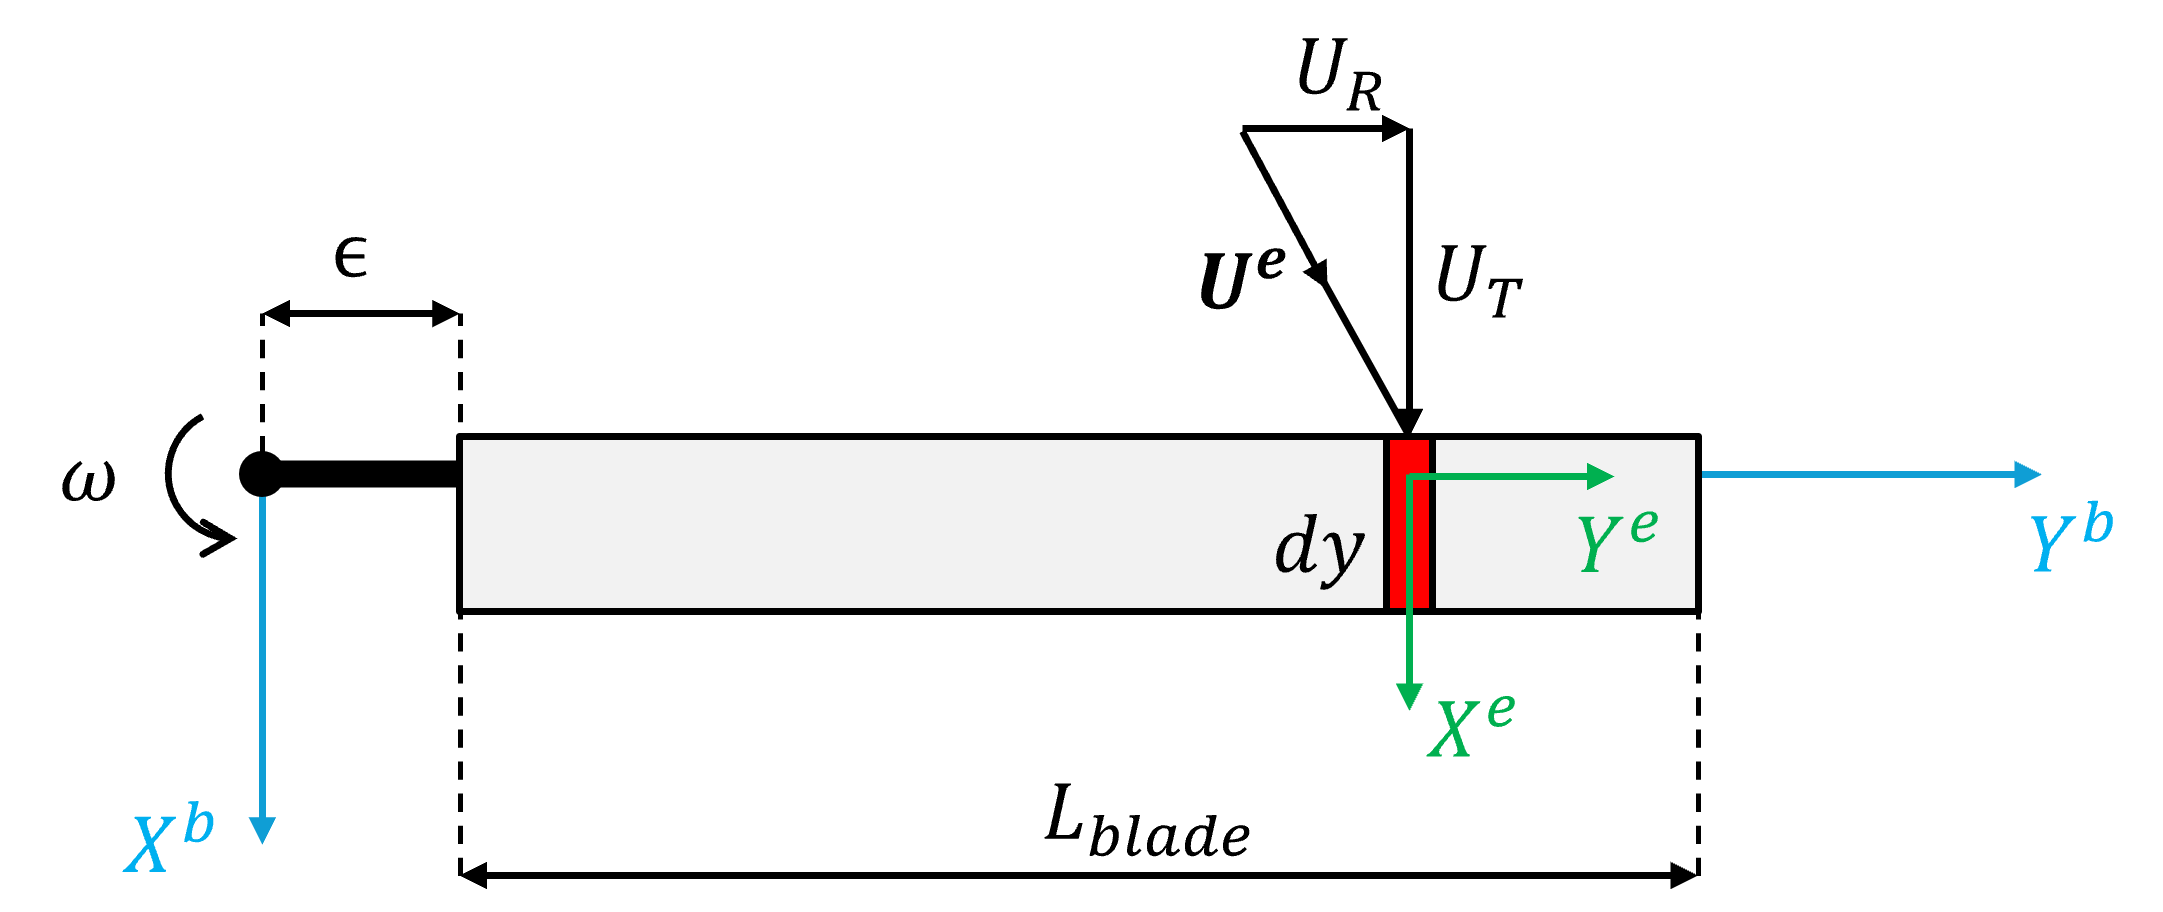
\includegraphics[width=9cm]{Figures/implementation/bet/blade_model.png}
        \caption{Image \textcolor{blue}{falta trocar as referencias dos eixos}}
\end{figure}


\subsection{Blade forces and moments}
\label{section:bem_forces_moments}

\textcolor{blue}{Forces in Element Frame}

\begin{equation}
    (\mathrm{d}L^{e})_n = \frac{1}{2} \rho \cdot   \|  \left( \mathbf{V}^e \right)_n \| ^2 dy
    \label{eq:elementary_lift}
\end{equation}

\begin{equation}
    (\mathrm{d}D^{e})_n = \frac{1}{2} \rho \left[ C_d \right] \|  \left( \mathbf{V}^e \right)_n \| ^2 dy
    \label{eq:elementary_drag}
\end{equation}

\textcolor{blue}{Blade Force in Blade Frame}

\begin{equation}
    \left(\mathbf{T}^{b}\right)_m = \int_\epsilon^R \left( \mathrm{d}\mathbf{F}^{e}\right)_n \, \mathrm{d}y
\end{equation}

\begin{equation}
    \left(\mathbf{T}^{b}\right)_m = \int_\epsilon^R \left(\mathbf{r}^e \right)_n \times \left( \mathrm{d}\mathbf{F}^{e}\right)_n \, \mathrm{d}y
\end{equation}


\begin{equation}
    \left(\mathbf{r}^e \right)_n = \begin{bmatrix} 0 & n \cdot \left(\frac{L_{rotor}}{N_e}\right) & 0 \end{bmatrix}^T
\end{equation}



\textcolor{blue}{Blade Force in Rotor Frame}

\begin{figure}[!htb]
    \centering
        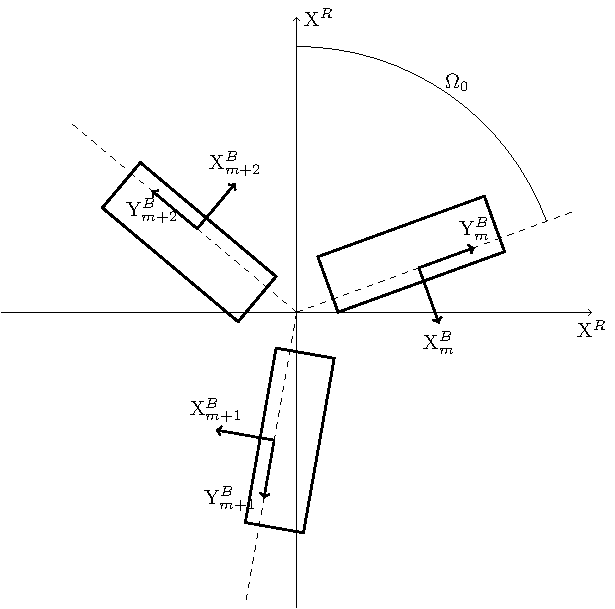
\includegraphics[width=8cm]{Figures/implementation/bet/blade_forces/multiple_blades_reference.pdf}
        \caption{Image \textcolor{blue}{falta trocar as referencias dos eixos}}
\end{figure}

\begin{equation}
    \left(\mathbf{F}^{r}\right)_m = Rot(\hat{\mathbf{z}}, \Omega_m) \cdot \left(\mathbf{F}^{b}\right)_m = Rot(\hat{\mathbf{z}}, \Omega_m) \cdot \int_\epsilon^R \left( \mathrm{d}\mathbf{F}^{e}\right)_n \, \mathrm{d}y
\end{equation}

\begin{equation}
    \left(\mathbf{T}^{r}\right)_m = Rot(\hat{\mathbf{z}}, \Omega_m) \cdot \left(\mathbf{T}^{b}\right)_m = Rot(\hat{\mathbf{z}}, \Omega_m) \cdot \int_\epsilon^R \left(\mathbf{r}^e \right)_n \times \left( \mathrm{d}\mathbf{F}^{e}\right)_n \, \mathrm{d}y
\end{equation}

%\begin{equation}
%	\Omega_m = \Omega_{0} +  m \cdot \frac{2\pi}{N_b}, \quad m \in \{0,1,2,\dots \}
%\end{equation}

\textcolor{blue}{Total Rotor Force and Torque in Rotor Frame}

\begin{equation}
    \mathbf{F}^{r} = \sum_m \left(\mathbf{F}^{r}\right)_m
\end{equation}


\begin{equation}
    \mathbf{T}^{r} = \sum_m \left(\mathbf{T}^{r}\right)_m 
\end{equation}


\textcolor{blue}{Forces in Blade Frame}

\begin{figure}[!htb]
    \centering
    \begin{minipage}{0.45\textwidth}
        \centering
        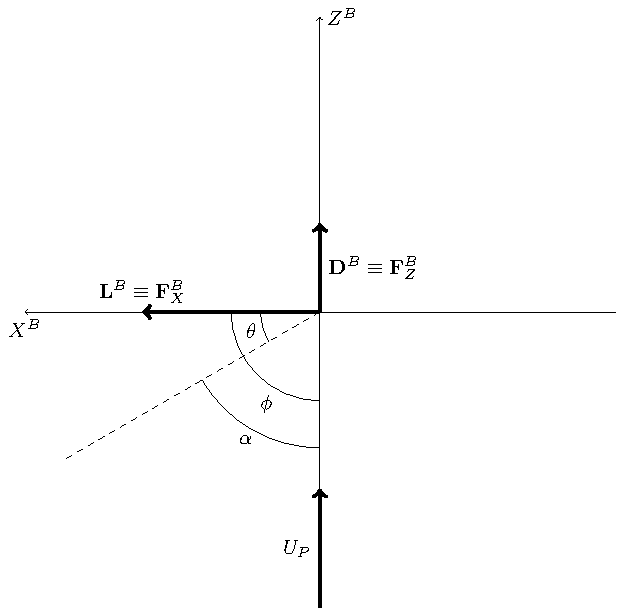
\includegraphics[width=\linewidth]{Figures/implementation/bet/blade_forces/blade_element_forces_1.pdf} % Replace with your image file
        \caption{Image 1}
    \end{minipage}
    \hfill
    \begin{minipage}{0.45\textwidth}
        \centering
        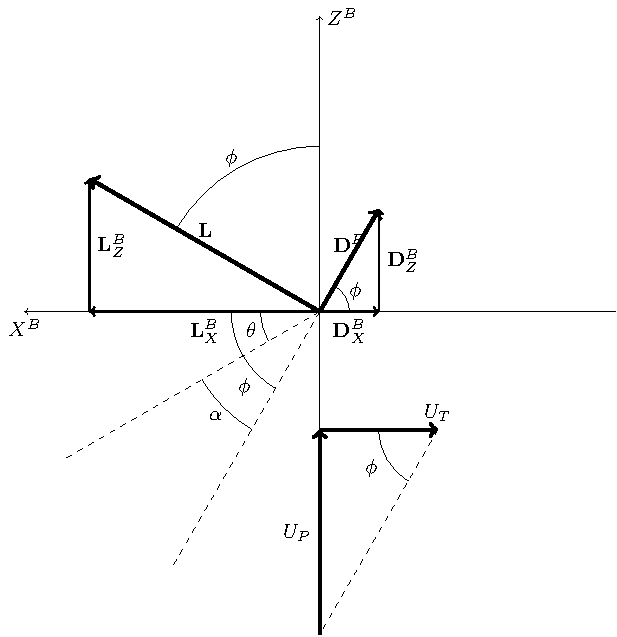
\includegraphics[width=\linewidth]{Figures/implementation/bet/blade_forces/blade_element_forces_2.pdf} % Replace with your image file
        \caption{Image 2}
    \end{minipage}
    \vfill
    \begin{minipage}{0.45\textwidth}
        \centering
        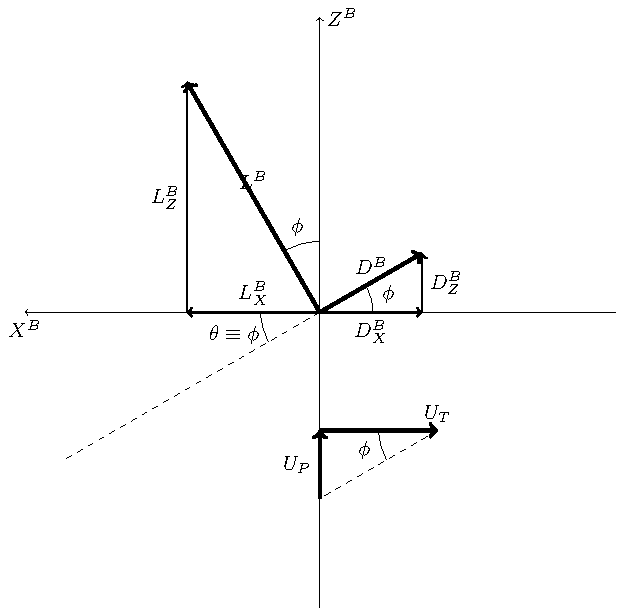
\includegraphics[width=\linewidth]{Figures/implementation/bet/blade_forces/blade_element_forces_3.pdf} % Replace with your image file
        \caption{Image 3}
    \end{minipage}
    \hfill
    \begin{minipage}{0.45\textwidth}
        \centering
        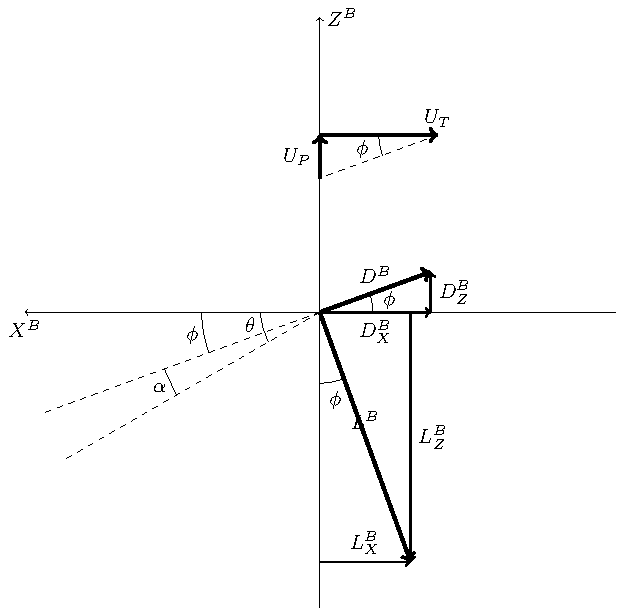
\includegraphics[width=\linewidth]{Figures/implementation/bet/blade_forces/blade_element_forces_4.pdf} % Replace with your image file
        \caption{Image 4}
    \end{minipage}
    \caption{2x2 Grid of Images \textcolor{blue}{falta trocar as referencias dos eixos}}
\end{figure}


\begin{figure}[!htb]
    \centering
    \begin{minipage}{0.45\textwidth}
        \centering
        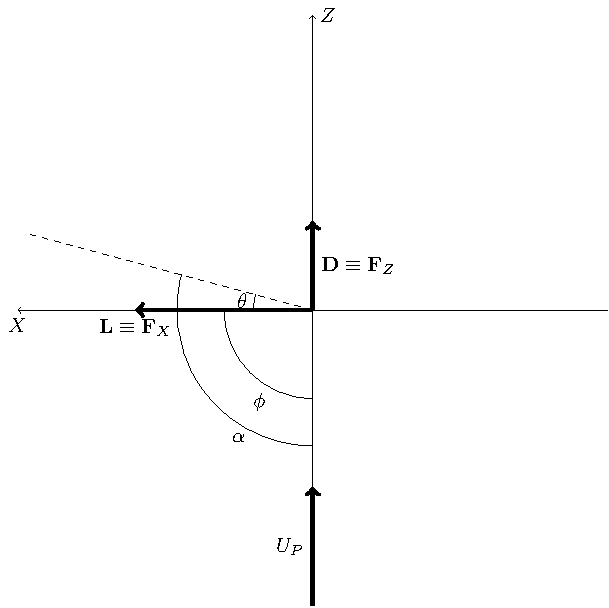
\includegraphics[width=\linewidth]{Figures/implementation/bet/blade_forces/blade_element_forces_5.pdf} % Replace with your image file
        \caption{Image 1}
    \end{minipage}
    \hfill
    \begin{minipage}{0.45\textwidth}
        \centering
        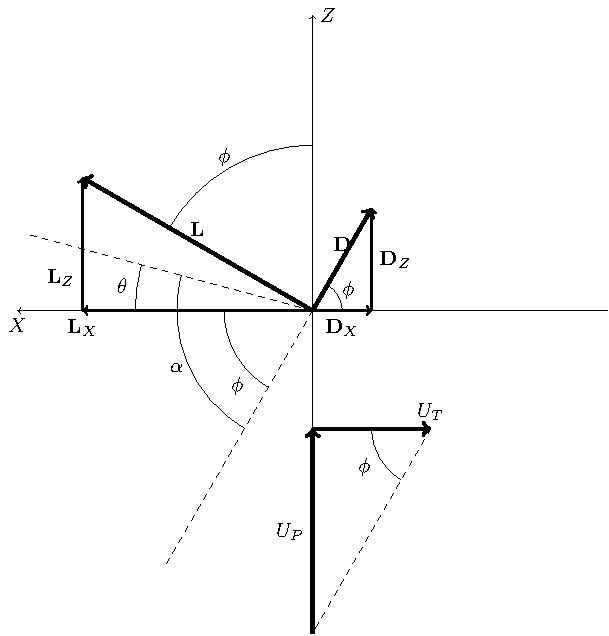
\includegraphics[width=\linewidth]{Figures/implementation/bet/blade_forces/blade_element_forces_6.pdf} % Replace with your image file
        \caption{Image 2}
    \end{minipage}
    \caption{1x2 Grid of Images \textcolor{blue}{falta trocar as referencias dos eixos}}
\end{figure}

\subsection{Velocities}

\textcolor{blue}{Element Velocity in  Element Frame}

\begin{equation}
    \mathbf{V}^i = Rot(E_A)  \mathbf{V}^v \implies \mathbf{V}^v = Rot(E_A)^{-1} \mathbf{V}^i
\end{equation}

$$
    \text{Element Velocity} = \text{Vehicle Translation} + \text{Vehicle Rotation } + \text{Rotor Rotation} + \text{Induced Velocity}
$$


\begin{equation}
    \left( \mathbf{V}^e \right)_n =  \underbrace{\boldsymbol{V}^e_T}_\text{Vehicle Translation} + \underbrace{\left(\mathbf{r}_{CM}\right)_n \times \boldsymbol{\omega}^v_{vehicle}}_\text{Vehicle Rotation } + \underbrace{\left(\mathbf{r}^e\right)_n \times \boldsymbol{\omega}^r_{rotor}}_\text{Rotor Rotation} + \underbrace{\boldsymbol{v}_{i}^r}_\text{Induced Velocity}
\end{equation}


\textcolor{blue}{Velocidade de translação}



\begin{equation}
    \mathbf{P}^e =  \boldsymbol{R}^*_{v \rightarrow e} \mathbf{P}^v 
\end{equation}

\begin{equation}
    \mathbf{V}^e_T \equiv \frac{\mathrm{d}\mathbf{P}^e}{\mathrm{d}t} =  \frac{\mathrm{d}}{\mathrm{d}t} \left(\boldsymbol{R}^*_{v \rightarrow e} \mathbf{P}^v \right) \implies  \mathbf{V}^e_T = \boldsymbol{\dot{R}}^*_{v \rightarrow e} \mathbf{P}^v + \boldsymbol{R}^*_{v \rightarrow e} \dot{\mathbf{P}}^v
\end{equation}

\begin{equation}
    \mathbf{V}^e_T = \dot{\boldsymbol{R}}^*_{v \rightarrow e} \mathbf{P}^v + \boldsymbol{R}^*_{v \rightarrow e} \mathbf{V}^v
\end{equation}

\subsubsection{Induced Velocity}

\textcolor{blue}{Windmill Break State}

\begin{equation}
    {\frac{v_{i}}{v_{h}}}=-\left({\frac{V_{c}}{2v_{h}}}\right)-{\sqrt{\left({\frac{V_{c}}{2v_{h}}}\right)^{2}-1}},
\end{equation}

\textcolor{blue}{Vortex Ring State}

\begin{equation}
    \frac{v_{i}}{v_{h}}=\kappa+k_{1}\left(\frac{V_{c}}{v_{h}}\right)+k_{2}\left(\frac{V_{c}}{v_{h}}\right)^{2}+k_{3}\left(\frac{V_{c}}{v_{h}}\right)^{3}+k_{4}\left(\frac{V_{c}}{v_{h}}\right)^{4}
\end{equation}

\textcolor{blue}{Como o $v_i$ é escrito no referencial do rotor, e o referencial do rotor está alinha com o referencial do veiculo, então não é necessário converter entre referencais, apenas criar um vetor com componente vertical. Como a velocidade induzida é para a parte de baixo do rotor, então fica com componente negativa}

\begin{equation}
   \boldsymbol{v}_{i}^v \equiv \boldsymbol{v}_{i}^r = \begin{bmatrix} 0 & 0 & -v_i \end{bmatrix}^T
\end{equation}



\section{AERODAS Model}
\label{section:aerodynamic_model}

\textcolor{blue}{Motivar a necessidade de haver um modelo aerodinâmico}

As seen in section \ref{section:bem_forces_moments}, the \gls{bet} is a based model, in short words, defined a sum of elementary 2D airfoil setions. Then its crucial for its implementation a computational method to obtain $\left[ C_l \right]$ and $\left[ C_d \right]$ for 2D airfoils, in equations \ref{eq:elementary_lift} and \ref{eq:elementary_drag}.

\textcolor{blue}{questões computacionais}

Also \gls{bet} has critical consideration rather the number of elements used to define a blade. The higher the number of elements, the higher the number of calculations needed to be perform a rotor analysis. This means that for a time-dependent model as a free-fall considered in this work, more critical it is, in term of computational time, to perform any simulation. So a fast model should be used.

\textcolor{blue}{altos angulos de ataque}

For choosing a airfoil analysis, one must consider the rotor dynamics. In this study, the rotor is under the phenomena of autorotation which has its displacement mainly in descent direction, then some considerations should be made about the angles of attack. On blade's root, the angular velocity is smaller when compared to the blade's tip. Meaning, the inflow angle is mainly composed by a vertical component rather than a horizontal component. So, a wider range of angles of attack should be considered. Also, if it is considered a pure vertical descent mode and small rotor angular velocity, the angles of attack while certainly be near 90$^{\circ}$ meaning that the rotor will work on a stall model. A reference to the pitch angle, $\theta$, and the blade twist should be made, however for thin airfoils it is known that for angles near 20~30$^{\circ}$, depending on thickness and camber, the airfoils starts to operate as a flate plate on stall mode, with completely separate boundary layers.

\textcolor{blue}{apresentação do aerodas}

This consideration are needed in other aerodynamic applications of rotors operating in high angles of attack, namely in wind turbines. So, David A. Spera developed an aerodynamic model \cite{spera_models_2008} naned AERODAS, for to predict lift and drag coefficients for stallel and unstalled airfoils. 

The development of horizontal-axis wind turbines is described in this article as a result of a Department of Energy-sponsored and NASA-led federal effort that ran from 1973 to 1995. This study develops an empirical model for airfoil lift and drag by fitting test data with algebraic equations, rather than using aerodynamic theory. It includes a wide range of conditions such as different airfoils, Reynolds numbers, and angles of attack, and also models circular cylinders and thin plates. Key improvements include expanding the test data set to cover more airfoils and configurations. Unlike previous models, it uses empirical equations derived from actual airfoil behavior at high angles of attack in the post-stall regime, rather than assuming flat plate behavior. 

The model also considers airfoil thickness in addition to aspect ratio and angle of attack. Its accuracy is evaluated by calculating the mean and standard deviation of the lift and drag data across various airfoils. Finally, the model is applied in Blade Element Momentum (BEM) analysis to predict wind turbine power and fan performance, and its results are compared with measured data to evaluate its effectiveness.

\textcolor{blue}{modelo}

Going deeper into the mathematical prespective, the AERODAS model main goal is to get the lift, $C_l$, and drag,$C_d$, curves as function of angle of attack, $\alpha$. Figure \ref{fig:aerodas_functions} presents the considered curves and highlight the major considerations about the model.

\begin{figure}[!htb]
    \centering
    \subfloat[AERODAS model lift coefficient,$C_l$, as functio of angle of attack,$\alpha$, from \cite{spera_models_2008}\label{fig:aerodas_cl}]{
        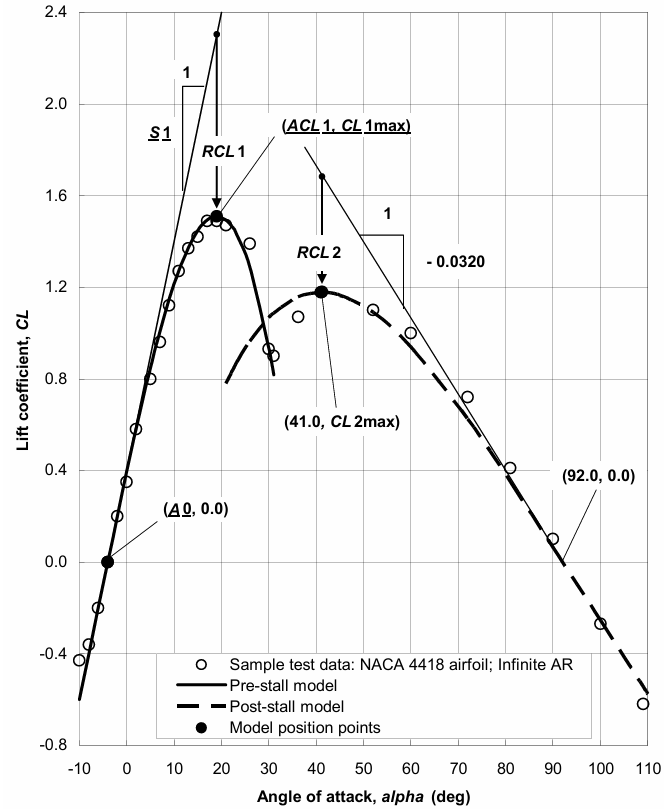
\includegraphics[height=8.5cm]{Figures/implementation/bet/aerodas/aerodas_cl_model.png}
    }\hfill
    \subfloat[AERODAS model drag coefficient,$C_d$, as functio of angle of attack,$\alpha$, from \cite{spera_models_2008}\label{fig:aerodas_cd}]{
        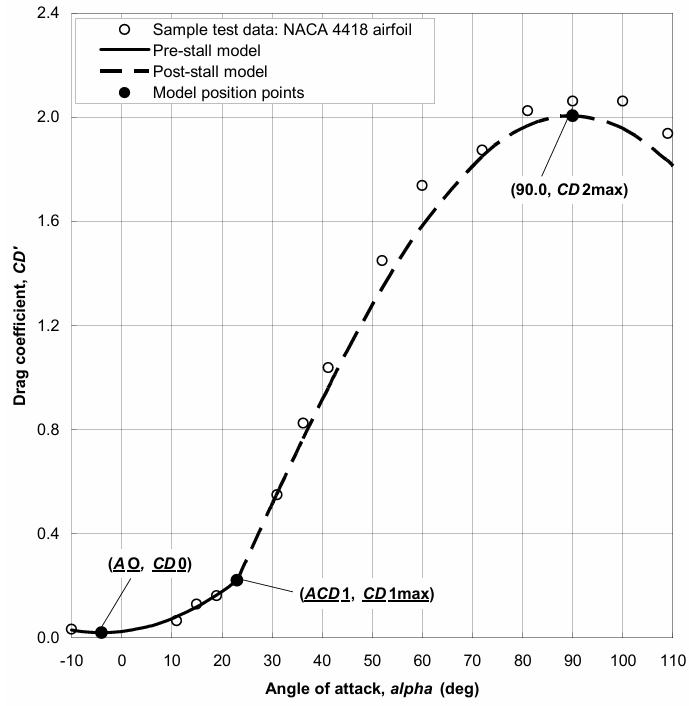
\includegraphics[height=8.5cm]{Figures/implementation/bet/aerodas/aerodas_cd_model.png}
    }
    \caption{AERODAS model curves}
    \label{fig:aerodas_functions}
\end{figure}

From \cite{spera_models_2008}, the main equations for the model are presented in table \ref{tab:aerodas_key_equation}. The key point of AERODAS model is separate the lift and drag curve with equations for pre-stall and post stall regimes. 

\textcolor{blue}{equações de lift}

For lift it is defined mathematical expressions for pre-stall, $CL1$, considering the Spera \cite{spera_models_2008} uses a proposed model by Viterna, where it consideres a linear variation for the lift coefficient, $S1$, and while $\alpha$ increases approaching the stall angle $ACL1$, the function uses a reduction from extension of linear segment of lift curve to $CL1_{max}$ (maxima $CL$ value, before stall), $RCL1$, 

% Please add the following required packages to your document preamble:
% \usepackage{multirow}
\begin{table}[!htb]
    \centering
    \renewcommand{\arraystretch}{2.5} % Aumenta o espaço entre as linhas
    \footnotesize % Reduz o tamanho da fonte (use \footnotesize ou \scriptsize se quiser menor ainda)
    \begin{tabular}{llll}
        \hline
        Mode                        & Coefficient                                     & Condition                                   & Equation                                                                                                                    \\ \hline
        \multirow{4}{*}{Pre-stall}  & \multicolumn{1}{c}{\multirow{2}{*}{Lift $CL1$}} & $\alpha \geq A0$                            & $C L1=S1\cdot\left(\alpha-A0\right)-R C L1\left(\frac{\alpha-A0}{A C L1-A0}\right)^{N1}$                                    \\
                                    & \multicolumn{1}{c}{}                            & $\alpha < A0$                               & $CL1=S1\cdot(\alpha-A0)+R C L1\left(\frac{A0-\alpha}{A C L1-A0}\right)^{N1}$                                                \\ \cline{2-4} 
                                    & \multirow{2}{*}{Drag $CD1$}                     & $(2 A0 - ACD1) \leq \alpha \leq ACD1$       & $C D1=C D0+\left(C D1\operatorname*{max}-C D0\right)\left({\frac{\alpha-A0}{A C D1-A0}}\right)^{M}$                         \\
                                    &                                                 & $\alpha < (2 A0 - ACD1)$ or $\alpha > ACD1$ & $CD1=0$                                                                                                                     \\ \hline
        \multirow{7}{*}{Post-stall} & \multicolumn{1}{c}{\multirow{4}{*}{Lift $CL2$}} & $0 < \alpha < ACL1$                         & $CL2=0$                                                                                                                     \\
                                    & \multicolumn{1}{c}{}                            & $ACL1 \leq \alpha \leq 92^{\circ}$          & $CL2=-0.032\left(\alpha-92.0\right) - RCL2\cdot\left({\frac{92.0-\alpha}{51.0}}\right)^{N2}$                                \\
                                    & \multicolumn{1}{c}{}                            & $\alpha > 92^{\circ}$                       & $CL2=-0.032\left(\alpha-92.0\right) + RCL2 \cdot \left(\frac{\alpha-92.0}{51.0}\right)^{N2}$                                \\
                                    & \multicolumn{1}{c}{}                            & $\alpha < 0$                                & $CL2[\alpha] = - CL2[-\alpha + 2 \cdot A0]$                                                                                 \\ \cline{2-4} 
                                    & \multirow{3}{*}{Drag $CD2$}                     & $(2A0-ACL1) \leq \alpha \leq ACL1$          & $CD2 = 0$                                                                                                                   \\
                                    &                                                 & $\alpha \geq ACD1$                          & $\begin{aligned}CD2 = CD1_{max}+\left( CD2_{max} - CD1_{max}\right) \cdot \\ \cdot \sin\left({\frac{\alpha-A C D1}{90.0-A C D1}} \cdot 90.0\right)\end{aligned}$ \\
                                    &                                                 & $\alpha \leq (2A0 - ACD1)$                  & $CD2\big[ \alpha \big] = CD2 \big[- \alpha + A0\big]$                                                                       \\ \hline
        \end{tabular}
    \caption{AERODAS model main equations \cite{spera_models_2008}}
    \label{tab:aerodas_key_equation}
\end{table}

\begin{equation}
    R C L1=S1\cdot(A C L1-A0)-C L1\,\mathrm{max}
\end{equation}

and exponent defining shape of lift curve at $ACL1_{max}$, $N1$,

\begin{equation}
    N1 = 1 + CL1_{max} / RCL
\end{equation}

In post-stall regime, the lift curve, $CL2$, is modeled by an equation of the same shape as in the pre-stall regime, but with a reversed slope. In this case, the reduction from extension of linear segment of lift curve to $CL2_{max}$

\begin{equation}
    RCL2 = -0.032 \left(41.0-92.0\right) - CL2_{max} = 1.632- CL2_{max}
\end{equation}

and exponent defining shape of lift curve at $CL2_{max}$, $N1$,

\begin{equation}
    N2 = 1 + CL2 / RCL2
\end{equation}


\textcolor{blue}{equações de drag}

For drag coefficient, its behavior is usually defined considering a quadatic expression \cite{spera_models_2008}. So, AEDODAS model uses 

\begin{equation}
    M = 2
\end{equation}

\textcolor{blue}{Post-Stall Maximum Lift and Drag}

The mais goal of AERODAS is to compute the post-stall coefficients of which theres no available experimental data. So to extrapolate data, AERODAS uses two parameteres defining the maximum lift, $CL2_{max}$, and drag, $CD2_{max}$, to compute post-stall curves. To accomplish this goal \cite{spera_models_2008} considers  that this coefficients are functions of thickness-to-chord ratio, $t/c$ , and its aspect ratio, $AR$.

\begin{equation}
    CL2_{max} = F1 \left[ t/c \right] \cdot F2 \left[ AR \right]] \quad \text{and} \quad CD2_{max} = G1 \left[ t/c \right] \cdot G2 \left[ AR \right]
\end{equation}

For lift coefficient, empirical equations developed follows:

\begin{equation}
    F1=1.190\cdot\left[1.0-\left(t/c\right)^{2}\right] \quad \text{and} \quad F2= 0.65 + 0.35\,\mathrm{exp}\left[-\left(9.0\slash{A}R\right)^{2.3}\right]
\end{equation}

For instance, the empirical equations for maximum drag are

\begin{equation}
    G_1 = 2.300\cdot\,\mathrm{exp}\left\{-\left[0.65\left(\frac{t}{v}\right)\right]^{0.90}\right\} \quad \text{and} \quad G_2 = 0.52 + 0.48\,\mathrm{exp}\left[-\left(\frac{6.5}{A R}\right)^{1.1}\right]
\end{equation}



\textcolor{blue}{Lift and Drag Model Configurations}

Once the model consideres coefficients equations in the pre-stall and post-stall regimes separately, it is necessary to select the correct one. This consideration is necessary once for $\alpha \geq ACL1$ (post-stall regime) theres is an overlap between the $CL1$ and $CL2$. For $\alpha < ACL1$ (pre-stall regime), $CL2$ is consider 0, then $CL1$ is the correct expresstion, for the pre-stall regime.

If $\alpha \geq A0$

\begin{equation}
    C L=\operatorname*{max}(CL1, CL2)
\end{equation}

If $\alpha \leq A0$

\begin{equation}
    CL = \operatorname*{min}(CL1 , CL2) \quad \text{and} \quad CD = \operatorname*{max}(CD1, CD2)
\end{equation}


\textcolor{blue}{XFLR5 Data  Aeroda Model  Input}

Some parameteres such as  angle of attack at which $CL1 = 0$, $A0$, angle of attack at maximum pre-stall lift $ACL1$ and slope of linear segment of pre-stall lift curve, $S1$, for $CL$ curve and minimum drag coefficient at $\alpha = A0$, $CD0$, and angle of attack at maximum pre-stall drag, $ACD1$, are necessary data parameters, either from simulation or windtunnel tests, to compute AERODAS model. Also, it is important to note that both maximum pre-stall lift coefficient, $CL1_{max}$, and maximum pre-stall drag coefficient at $ACD1 = 0$,  $CD1_{max}$, are another necessary parameters from simulation or windtunnel data.

This parameters are key for AERODAS, once it is considered that no data for angles in the stall regime is available. So its purpose is to extrapole data using  equations presented in tabel \ref{tab:aerodas_key_equation}, and further parameters are used to. In this sense, it is used simulation data from XFLR5 as input data for obtaining AERODAS parameters.

In appendix \ref{chapter:aerodas_xflr5} the complete process to extract data from XFLR5 is presented. This is only a programming problem and out of the scope for this work, though in this appendix it is explain in detail how to convert simulation data, with a alot of information, to a simple table with some parameter values for some Reynolds Number.

\textcolor{blue}{Explicar o modelo aerodinâmico do XFLR5}

As last topic about the 2D aerodynamic model for \gls{bet} using aerodas is to understande what is behind the XFLR5 code and what is is validity to the problem. XFLR5 is a ...

\subsection{Prandtl Tip Losses}
\label{section:prandtl_tip}


%%%%%%%%%%%%%%%%%%%%%%%%%%%%%%%%%%%%%%%%%%%%%%%%%%%%%%%%%%%%%%%%%%%%%%%%
\section{Atmosphere Model}
\label{section:atmosphere_model}

The 2D aerodynamic loads $\mathrm{d}L$, eq. \ref{eq:elementary_lift}, and  $\mathrm{d}D$, eq. \ref{eq:elementary_drag}, are directly proportional to the air density, $\rho$. Also, the atmospheric proprieties during the flight change with altitude. In this sense, a atmospheric model is necessary to compute the aerodynamic loads.

On the literature there are many atmospheric models such as the \gls{isa} \cite{noauthor_iso_nodate}, \gls{nasa}'s \gls{eam} \cite {noauthor_earth_nodate} and \gls{e-gram} \cite{white_earth_2021}, and NRLMISES00 \cite{picone_nrlmsise00_2002}.

\begin{figure}[!htb]
	\centering
	\begin{minipage}{0.48\textwidth}
		\centering
		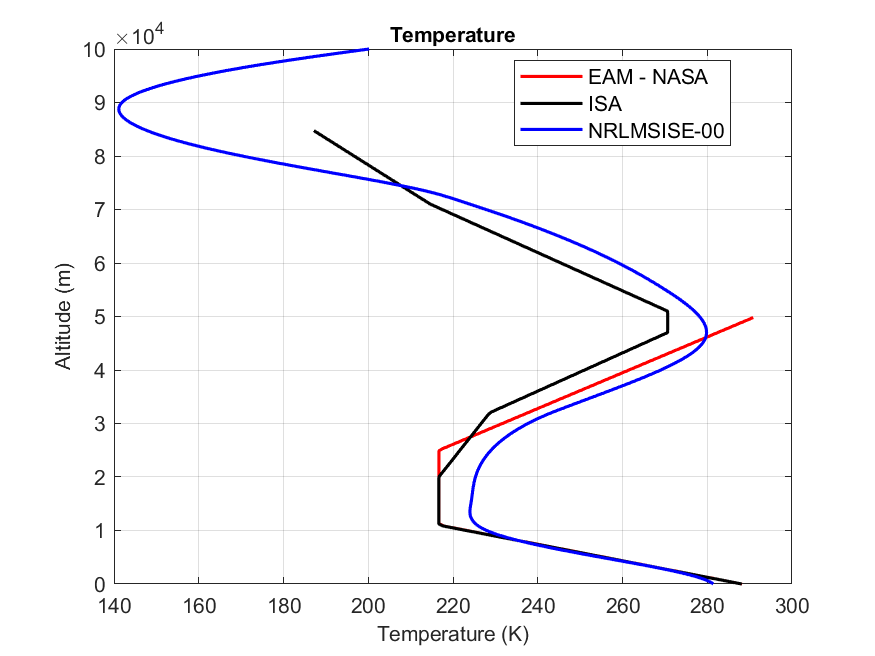
\includegraphics[width=\textwidth]{Figures/implementation/atmos/temperature_plot.png}
		\caption{Temperature Comparison}
		\label{fig:atmos_models_comp_temp}
	\end{minipage}
	\hfill
	\begin{minipage}{0.48\textwidth}
		\centering
		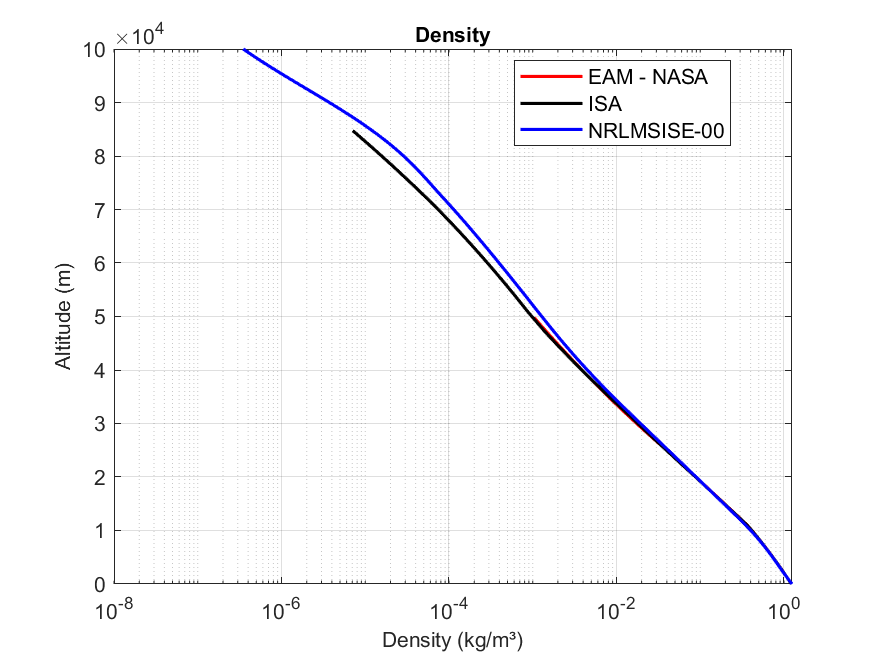
\includegraphics[width=\textwidth]{Figures/implementation/atmos/density_plot.png}
		\caption{Density Comparison}
		\label{fig:atmos_models_comp_density}
	\end{minipage}
\end{figure}


\begin{table}[!htb]
    \centering
    \begin{tabular}{
    >{\columncolor[HTML]{FFFFFF}}l 
    >{\columncolor[HTML]{FFFFFF}}r
    >{\columncolor[HTML]{FFFFFF}}r
    >{\columncolor[HTML]{FFFFFF}}r }
    \hline
    {\color[HTML]{000000} No. Function Calls} & \multicolumn{1}{r}{\cellcolor[HTML]{FFFFFF}{\color[HTML]{000000} EAM \cite{noauthor_iso_nodate}}} & \multicolumn{1}{r}{\cellcolor[HTML]{FFFFFF}{\color[HTML]{000000} ISA \cite{noauthor_earth_nodate}}} & \multicolumn{1}{r}{\cellcolor[HTML]{FFFFFF}{\color[HTML]{000000} NRLMISES00 \cite{picone_nrlmsise00_2002}}} \\ \hline
    {\color[HTML]{000000} 1}                  & {\color[HTML]{000000} 0.8 \unit{\m\second}}                                                                                           & {\color[HTML]{000000} 25.1 \unit{\m\second}}                                                                                        & {\color[HTML]{000000} 46.6 \unit{\m\second}}                                                                                                  \\
    {\color[HTML]{000000} 10}                 & {\color[HTML]{000000} 1.0 \unit{\m\second}}                                                                                           & {\color[HTML]{000000} 5.1 \unit{\m\second}}                                                                                           & {\color[HTML]{000000} 25.0 \unit{\m\second}}                                                                                                 \\
    {\color[HTML]{000000} 100}                & {\color[HTML]{000000} 0.1 \unit{\m\second}}                                                                                           & {\color[HTML]{000000} 19.1 \unit{\m\second}}                                                                                          & {\color[HTML]{000000} 173.7 m\unit{\m\second}}                                                                                                \\
    {\color[HTML]{000000} 1000}               & {\color[HTML]{000000} 0.4 \unit{\m\second}}                                                                                           & {\color[HTML]{000000} 173.9 m\unit{\m\second}}                                                                                         & {\color[HTML]{000000} 1.6 \unit{\second}}                                                                                                   \\
    {\color[HTML]{000000} 10000}              & {\color[HTML]{000000} 3.0 \unit{\m\second}}                                                                                           & {\color[HTML]{000000} 1.3 \unit{\second}}                                                                                             & {\color[HTML]{000000} 21.0 \unit{\second}}                                                                                                  \\
    {\color[HTML]{000000} 100000}             & {\color[HTML]{000000} 28.1 \unit{\second}}                                                                                          & {\color[HTML]{000000} 18.1 \unit{\second}}                                                                                           & {\color[HTML]{000000} 3.7 \unit{\minute}}                                                                                                 \\ \hline
    \end{tabular}
    \caption{Computational times for different number of function calls for the three atmospheric models.}
\end{table} 








 % file "Thesis_Implementation.tex"
\clearpage

%%%%%%%%%%%%%%%%%%%%%%%%%%%%%%%%%%%%%%%%%%%%%%%%%%%%%%%%%%%%%%%%%%%%%%%%
%                                                                      %
%     File: Thesis_Implementation.tex                                  %
%     Tex Master: Thesis.tex                                           %
%                                                                      %
%     Author: Andre C. Marta                                           %
%     Last modified :  4 Mar 2024                                      %
%                                                                      %
%%%%%%%%%%%%%%%%%%%%%%%%%%%%%%%%%%%%%%%%%%%%%%%%%%%%%%%%%%%%%%%%%%%%%%%%

\chapter{Computational Methodology}
\label{chapter:computational_methodology}


%%%%%%%%%%%%%%%%%%%%%%%%%%%%%%%%%%%%%%%%%%%%%%%%%%%%%%%%%%%%%%%%%%%%%%%%
\section{Solvers}
\label{section:solvers}

%%%%%%%%%%%%%%%%%%%%%%%%%%%%%%%%%%%%%%%%%%%%%%%%%%%%%%%%%%%%%%%%%%%%%%%%
\section{Application Development and Workflow}
\label{section:development_workflow}

%%%%%%%%%%%%%%%%%%%%%%%%%%%%%%%%%%%%%%%%%%%%%%%%%%%%%%%%%%%%%%%%%%%%%%%%
\section{Experimental tests}
\label{section:experimental_tests}	 % file "Thesis_ComputationalMethodology.tex"
\clearpage


%%%%%%%%%%%%%%%%%%%%%%%%%%%%%%%%%%%%%%%%%%%%%%%%%%%%%%%%%%%%%%%%%%%%%%%%
%                                                                      %
%     File: Thesis_Results.tex                                         %
%     Tex Master: Thesis.tex                                           %
%                                                                      %
%     Author: Andre C. Marta                                           %
%     Last modified :  4 Mar 2024                                      %
%                                                                      %
%%%%%%%%%%%%%%%%%%%%%%%%%%%%%%%%%%%%%%%%%%%%%%%%%%%%%%%%%%%%%%%%%%%%%%%%

\chapter{Results}
\label{chapter:results}
 % file "Thesis_Results.tex"
\clearpage

%%%%%%%%%%%%%%%%%%%%%%%%%%%%%%%%%%%%%%%%%%%%%%%%%%%%%%%%%%%%%%%%%%%%%%%%
%                                                                      %
%     File: Thesis_Conclusions.tex                                     %
%     Tex Master: Thesis.tex                                           %
%                                                                      %
%     Author: Andre C. Marta                                           %
%     Last modified :  4 Mar 2024                                      %
%                                                                      %
%%%%%%%%%%%%%%%%%%%%%%%%%%%%%%%%%%%%%%%%%%%%%%%%%%%%%%%%%%%%%%%%%%%%%%%%

\chapter{Conclusions}
\label{chapter:conclusions}

Insert your chapter material here.


% ----------------------------------------------------------------------
\section{Achievements}
\label{section:achievements}

The major achievements of the present work.


% ----------------------------------------------------------------------
\section{Future Work}
\label{section:future}

A few ideas for future work.

 % file "Thesis_Conclusions.tex"
\clearpage

% ----------------------------------------------------------------------
%  Bibliography
% ----------------------------------------------------------------------

% Add entry in the table of contents as chapter
\phantomsection
\addcontentsline{toc}{chapter}{\bibname}

% Include all references in .bib file, even non-cited ones...
%\nocite{*} % this should be used carefully because it is not correct!

% Produces the bibliography section when processed by BibTeX
%
% Bibliography style
% > entries ordered alphabetically
%\bibliographystyle{plain}
% > unsorted with entries appearing in the order in which the citations appear.
%\bibliographystyle{unsrt}
% > entries ordered alphabetically, with first names and names of journals and months abbreviated
%\bibliographystyle{abbrv}
% > entries ordered alphabetically, with reference markers based on authors' initials and publication year
%\bibliographystyle{alpha}
%
% Replacement bibliography styles provided by 'natbib' package
% (plainnat.bst, abbrvnat.bst, unsrtnat.bst )
% > entries ordered alphabetically
%\bibliographystyle{plainnat}
% > unsorted with entries appearing in the order in which the citations appear.
%\bibliographystyle{unsrtnat}
% > entries ordered alphabetically, with first names and names of journals and months abbreviated
%\bibliographystyle{abbrvnat} % <<<<< SELECT IF USING REFERENCES BY AUTHOR/YEAR
% > entries ordered alphabetically, with reference markers based on authors' initials and publication year
%\bibliographystyle{alpha}
%
% Custom bibliography style adapted from 'natbib' package
%   (based on http://tex.stackexchange.com/questions/5053/is-it-possible-to-get-unsrt-abbrv-bibliography)
%   (unsrtnat.bst + abbrvnat.bst -> abbrvunsrtnat.bst)
%   (original files copied from:
%   http://tug.ctan.org/macros/latex/contrib/natbib/abbrvnat.bst
%   http://tug.ctan.org/macros/latex/contrib/natbib/unsrtnat.bst
% > unsorted with entries appearing in the order in which the citations appear, with first names and names of journals and months abbreviated.
\bibliographystyle{abbrvunsrtnat} % <<<<< SELECT IF USING REFERENCES BY NUMBER (CITATION ORDER)

% External bibliography database file in the BibTeX format
\bibliography{Thesis_Bibliography_DB} % file "Thesis_Bibliography_DB.bib"

\cleardoublepage

% ----------------------------------------------------------------------
%  Appendix (optional)
%
%  CAUTION: 1) the main document (up to the conclusions) shall not exceed 80 pages
%           2) the document shall not exceed a total of 100 pages (per IST regulations)
% ----------------------------------------------------------------------
\appendix

% add page number prefix according to apendix chapter (optional)
\renewcommand{\thepage}{\thechapter.\arabic{page}}

% re-set arabic numbering (A.1,A.2,...) (optional, use only if chapter prefix is added)
\setcounter{page}{1}

\chapter{AERODAS Model Data from XFLR5}
\label{chapter:aerodas_xflr5}


\section{Dataset for AERODAS model}


\textcolor{blue}{explicação dos parametros mais importantes}


\section{Simulation Data as Model Inputs}

\textcolor{blue}{explicação de como é extraida a informação do XFLR5} % file "Thesis_Appendix_A.tex"
\cleardoublepage

% re-set arabic numbering (B.1,B.2,...) (optional, use only if chapter prefix is added)
%\setcounter{page}{1}

%%%%%%%%%%%%%%%%%%%%%%%%%%%%%%%%%%%%%%%%%%%%%%%%%%%%%%%%%%%%%%%%%%%%%%%%%
%                                                                      %
%     File: Thesis_Appendix_B.tex                                      %
%     Tex Master: Thesis.tex                                           %
%                                                                      %
%     Author: Andre C. Marta                                           %
%     Last modified :  4 Mar 2024                                      %
%                                                                      %
%%%%%%%%%%%%%%%%%%%%%%%%%%%%%%%%%%%%%%%%%%%%%%%%%%%%%%%%%%%%%%%%%%%%%%%%

\chapter{Technical Datasheets}
\label{chapter:appendixDatasheets}

It is possible to add PDF files to the document, such as technical sheets of some equipment used in the work.

% ----------------------------------------------------------------------
\section{Some Datasheet}
\label{section:datasheet}

See more options to include PDF files in \url{https://www.ctan.org/pkg/pdfpages}

% options:
%   pages : select pages to insert (listed and/or range)
%   nup : number of pages in the horizontal and vertical directions
%   landscape : rotate page
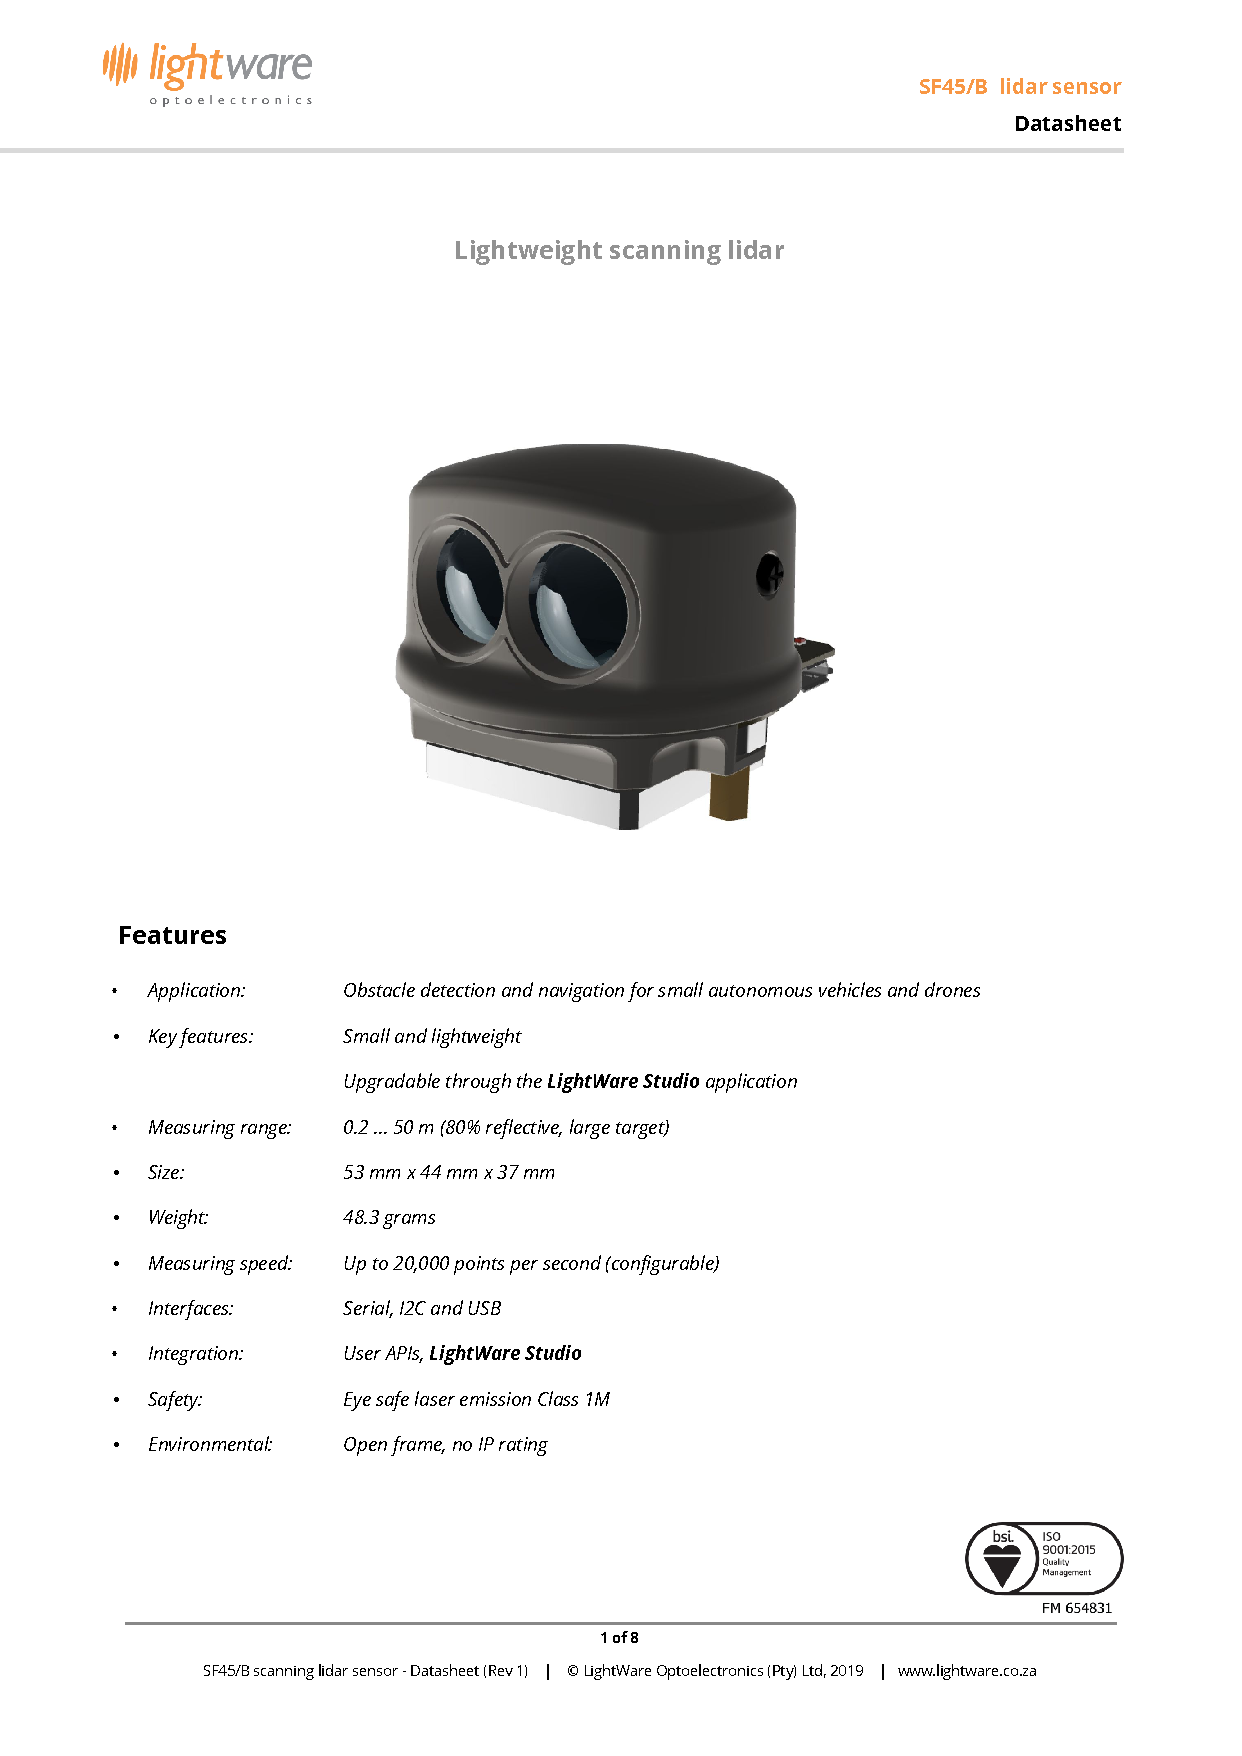
\includepdf[pages={1-4},nup=2x2,landscape=false]{Figures/datasheet_lidar.pdf}

 % file "Thesis_Appendix_B.tex"
%\cleardoublepage

% ----------------------------------------------------------------------
\end{document}
% ----------------------------------------------------------------------
